\باب{سمتی  قیمت تفاعل اور فضا میں حرکت}

\موٹا{سر سری جائزہ}\quad
جب کوئی جسم فضا میں حرکت کرتا ہو،   مساوات   \عددی{x=f(t)}، \عددی{y=g(t)} اور \عددی{z=h(t)}  جو اس جسم کے محدد  کو بطور وقت کا تفاعل  دیتی ہیں،  اس جسم کی راہ اور حرکت کی مقدار معلوم مساوات ہوں گی۔ سمتیہ   علامتیت  کی مدد سے ہم انہیں ایک مساوات \عددی{\kvec{r}(t)=f(t)\ai+g(t)\aj+h(t)\ak} کی صورت میں لکھ سکتے ہیں جو اس جسم کا مقام بطور وقت کا سمتی تفاعل دیتی ہے۔

اس باب میں  ہم احصاء استعمال کرتے ہوئے حرکت پذیر اجسام کی راہ، سمتی رفتار اور اسراع پر غور کریں گے۔ ہم  گولا،  سیارہ  اور مصنوعی سیارہ کی راہ اور حرکت کے عمومی سوالات کے جوابات جان سکے گے۔آخر حصہ میں ہم نیوٹن کے قوانین اور    تجاذب کی مدد سے سیاروں کی مدار کے  قوانین کپلر دریافت کریں گے۔ 


\حصہ{سمتی قیمت تفاعل اور فضائی منحنیات}\شناخت{حصہ_سمتی_تفاعل_سمتی_قیمت_تفاعل_اور_فضائی_منحنیات}
فضا میں متحرک ذرہ    کی حرکت جاننے کی خاطر ہم  مبدا سے  اس ذرہ  تک سمتیہ \عددی{\kvec{r}} لے کر \عددی{\kvec{r}} میں تبدیلی پر غور کرتے ہیں (شکل \حوالہ{شکل_سمتی_تفاعل_تعین_گر_سمتیہ})۔اگر اس ذرہ  کے محدد مقام  وقت کے ساتھ دو بار قابل تفرق ہوں،  تب  \عددی{\kvec{r}} بھی ایسا ہو گا، اور ہم کسی بھی لمحہ پر وقت کے لحاظ سے  \عددی{\kvec{r}}   کے  تفرق لے کر اس ذرہ  کی سمتی رفتار اور اسراع جان سکتے ہیں۔اگر ہمیں اس ذرہ  کی سمتیہ  سمتی رفتار یا سمتیہ  اسراع   بطور  وقت کے استمراری تفاعل معلوم ہو اور ہمیں ذرے کی ابتدائی  مقام اور سمتیہ رفتار کے بارے میں معقول معلومات ہو، تب ہم تکمل کی مدد سے، وقت کا تفاعل  \عددی{\kvec{r}} جان سکتے ہیں۔
\begin{figure}
\centering
\begin{minipage}{0.45\textwidth}
\centering
\pgfmathsetmacro{\a}{-0.25/360}
\pgfmathsetmacro{\ka}{1}
\pgfmathsetmacro{\b}{0.5/360}
\pgfmathsetmacro{\kb}{0.5}
\pgfmathsetmacro{\c}{1/360}
\pgfmathsetmacro{\d}{150}
\begin{tikzpicture}[font=\small,declare function={fx(\r,\t)=(\ka+\a*\t+\r*cos(\t));fy(\r,\t)=(\kb+\b*\t+\r*sin(\t));fz(\r,\t)=\c*\t;}]
\begin{axis}[clip=false,small,axis lines =center,view/h=135,xlabel={$x$},ylabel={$y$},zlabel={$z$},xlabel style={anchor=east},ylabel style={anchor=west},zlabel style={anchor=west},xtick={\empty},ytick={\empty},ztick={\empty},enlargelimits=true,xmin=0,ymin=0,
axis x line=none,axis y line=none,axis z line=none]
\addplot3[smooth,domain y=0:460,variable=\r,variable y=\t,samples y=50]({fx(1,t)},{fy(1,t)},{fz(1,t)});
\addplot3[-latex]coordinates {(0,0,0)({fx(1,\d)},{fy(1,\d)},{fz(1,\d)})}node[pos=0.5,yshift=1ex]{$\kvec{r}$}node[right]{$N(f(t),g(t),h(t))$}node[pos=0,left,yshift=1ex]{$O$};
\addplot3[-latex]coordinates {(0,0,0)(2,0,0)}node[left]{$x$};
\addplot3[-latex]coordinates {(0,0,0)(0,2,0)}node[right]{$y$};
\addplot3[-latex]coordinates {(0,0,0)(0,0,1)}node[left]{$z$};
\end{axis}
\end{tikzpicture}
\caption{فضا میں متحرک ذرہ کا تعین گر سمتیہ \عددی{\kvec{r}=\krightharpoonup{ON}} متغیر \عددی{t} کا تفاعل  ہو گا۔}
\label{شکل_سمتی_تفاعل_تعین_گر_سمتیہ}
\end{minipage}\hfill
\begin{minipage}{0.45\textwidth}
\centering
\begin{tikzpicture}[font=\small,declare function={fx(\ra,\t)=\ra*cos(\t);fy(\rb,\t)=\rb*sin(\t);fz(\rc,\t)=\rc*\t;}]
\pgfmathsetmacro{\h}{2.25}
\pgfmathsetmacro{\ra}{2}
\pgfmathsetmacro{\rb}{0.25*\ra}
\pgfmathsetmacro{\rc}{2/470}
\pgfmathsetmacro{\ta}{-110}
\pgfmathsetmacro{\tb}{0}
\pgfmathsetmacro{\tc}{180}
\pgfmathsetmacro{\td}{360}
\pgfmathsetmacro{\te}{-20}
\pgfmathsetmacro{\tf}{360+\ta}
\draw[-latex](0,0)--++(-145:2)node[left]{$x$};
\draw[-latex](0,0)--++(0:2.5)node[right]{$y$};
\draw[-latex](0,0)--++(0,3)node[left]{$z$};
\draw[thick,-stealth]([shift={(\ta:0.75cm and 0.185cm)}]0,0) arc (\ta:-20:0.75cm and 0.185 cm)node[pos=0.5,fill=white]{$t$};
 \draw[-latex](0,0,0)node[left,yshift=1ex]{$O$}--({fx(\ra,\te)},{fz(\rc,\te-\ta)+fy(\rb,\te)})node[circ]{}node[pos=0.4,above]{$\kvec{r}$};
 \draw[dashed,thick](0,0,0)--({fx(\ra,\te)},{fy(\rb,\te)})--({fx(\ra,\te)},{fz(\rc,\te-\ta)+fy(\rb,\te)});
\draw[dashed,domain=40:180,variable=\t]plot ({fx(\ra,\t)},{fy(\rb,\t)});
\draw[domain=180:360,variable=\t]plot ({fx(\ra,\t)},{fy(\rb,\t)});
\draw[domain=0:360,variable=\t]plot ({fx(\ra,\t)},{\h+fy(\rb,\t)});
\draw  ({fx(\ra,300)},{fy(\rb,300)})node[below]{$x^2+y^2=1$};
\draw(-\ra,0)--++(0,\h);
\draw(\ra,0)--++(0,\h);
\draw[domain=\ta:\tb,variable=\t]plot ({fx(\ra,\t)},{fz(\rc,\t-\ta)+fy(\rb,\t)});
\draw[dashed,domain=\tb:\tc,variable=\t]plot ({fx(\ra,\t)},{fz(\rc,\t-\ta)+fy(\rb,\t)});
\draw[domain=\tc:\td,variable=\t]plot ({fx(\ra,\t)},{fz(\rc,\t-\ta)+fy(\rb,\t)});
\draw  ({fx(\ra,\ta)},{fz(\rc,\ta-\ta)+fy(\rb,\ta)})node[circ]{}node[below,xshift=1ex]{$t=0$}node[left,xshift=-2ex,yshift=-1ex]{$(1,0,0)$};
\draw  ({fx(\ra,\tb)},{fz(\rc,\tb-\ta)+fy(\rb,\tb)})node[circ]{}node[right]{$t=\frac{\pi}{2}$};
\draw  ({fx(\ra,\tf)},{fz(\rc,\tf-\ta)+fy(\rb,\tf)})node[circ]{}node[below]{$t=2\pi$};
\draw[dashed] ({fx(\ra,\tf)},{fz(\rc,\tf-\ta)+fy(\rb,\tf)})-- (0,{fz(\rc,\tf-\ta)})node[circ]{}node[right]{$2\pi$};
\end{tikzpicture}
\caption{پیچدار منحنی \عددی{\kvec{r}(t)=(\cos t)\ai+(\sin t)\aj} کا بالائی نصف حصہ}
\label{شکل_سمتی_تفاعل_پیچدار}
\end{minipage}
\end{figure}
\جزوحصہء{تعریف}
جب وقفہ \عددی{I} کے دوران ایک ذرہ فضا میں حرکت  کرتا ہو، ہم اس ذرہ کے محدد جو وقت کے تفاعل ہو گے کی تعریف درج ذیل کرتے ہیں۔
\begin{align}\label{مساوات_سمتی_تفاعل_مقدار_معلوم_راہ}
x=f(t),\quad y=g(t),\quad z=h(t),\quad t\in I
\end{align}
نقاط \عددی{(x,y,z)=(f(t),g(t),h(t)),\,t\in I}  فضا میں وہ  \اصطلاح{منحنی} دیتے ہیں جنہیں ہم اس ذرے کی \اصطلاح{راہ}\فرہنگ{راہ}\حاشیہب{path}\فرہنگ{path} کہتے ہیں۔ مساوات \حوالہ{مساوات_سمتی_تفاعل_مقدار_معلوم_راہ} اس منحنی  کی \اصطلاح{مقدار معلوم روپ }\فرہنگ{مقدار معلوم!روپ}  ہے۔ مبدا سے ذرے  کے \اصطلاح{ مقام}  \عددی{N(f(t),g(t),h(t))}  تک لمحہ \عددی{t} پر   سمتیہ 
\begin{align*}
\kvec{r}(t)=\krightharpoonup{ON}=f(t)\ai+g(t)\aj+h(t)\ak
\end{align*} 
اس ذرے کا\اصطلاح{   تعین گر سمتیہ}\فرہنگ{تعین گر!سمتیہ}\حاشیہب{position vector}\فرہنگ{vector!position}  ہے۔تفاعل \عددی{f}، \عددی{g} اور \عددی{h}  تعین گر سمتیہ کے\اصطلاح{ اجزاء}  ہیں۔
 ذرے کی راہ سے مراد وقفہ \عددی{t} کے دوران   \عددی{\kvec{r}}  کی  پیداکردہ منحنی ہے۔


مساوات \حوالہ{مساوات_سمتی_تفاعل_مقدار_معلوم_راہ}  سمتیہ \عددی{\kvec{r}} کی تعریف وقفہ \عددی{I} پر  حقیقی متغیر \عددی{t} کی صورت میں دیتی ہے۔ زیادہ عمومی طور پر  دائرہ کار،   سلسلہ \عددی{D}،  پر  \اصطلاح{سمتی تفاعل}\فرہنگ{سمتی!تفاعل}\حاشیہب{vector function}\فرہنگ{vector!function} یا  \اصطلاح{سمتی  قیمت تفاعل}\فرہنگ{سمتی قیمت تفاعل}\حاشیہب{vector-valued function}\فرہنگ{vector-valued!function}   سے مراد وہ قاعدہ ہو گا   جو \عددی{D} کے  ہر رکن کو فضا میں ایک سمتیہ مختص کرتا ہو۔موجودہ استعمال میں دائرہ کار حقیقی اعداد  کے وقفوں    پر مشتمل ہوں  گے۔ بعد کے ایک باب میں دائرہ کار، مستوی یا فضا میں خطوں پر مشتمل ہوں گے   جہاں ہم  سمتی تفاعل کو سمتی میدان  کہیں گے۔

ہم حقیقی قیمت تفاعل کو \اصطلاح{غیر سمتی تفاعل}\فرہنگ{غیر سمتی! تفاعل}\حاشیہب{scalar functions}\فرہنگ{scalar!functions} کہتے ہیں تا کہ ان میں اور سمتی تفاعل میں فرق کرنا ممکن ہو۔  سمتیہ \عددی{\kvec{r}} کے اجزاء \عددی{t}  کے غیر سمتی تفاعل ہیں۔سمتی تفاعل کی تعریف  اس کے  ارکان تفاعل کی صورت میں دیتے وقت ہم فرض کرتے ہیں کہ   سمتی تفاعل کا دائرہ کار ہی  ارکان کے دائرہ کار   ہیں۔

\ابتدا{مثال}\ترچھا{پیچ دار تفاعل}\\
تمام حقیقی متغیر  \عددی{t} کے لئے سمتی تفاعل
\begin{align*}
\kvec{r}(t)=(\cos t)\ai+(\sin t)\aj+t\ak
\end{align*}
معین ہے اور  \عددی{\kvec{r}}   دائری نلکی \عددی{x^2+y^2=1} کے گرد  لپٹ کر چلتا ہے (شکل \حوالہ{شکل_سمتی_تفاعل_پیچدار})۔  سمتی تفاعل \عددی{\kvec{r}} کے \عددی{\ai} اور \عددی{\aj} اجزاء  جو \عددی{\kvec{r}} کے سر  کے  \عددی{x} اور \عددی{y} محدد ہیں   دائری نلکی  کی مساوات
\begin{align*}
x^2+y^2=(\cos t)^2+(\sin t)^2=1
\end{align*}
کو مطمئن کرتے ہیں لہٰذا \عددی{\kvec{r}} اس نلکی پر پایا جاتا ہے۔ متغیر \عددی{t} بڑھنے  \عددی{\ak}  جزو بڑھتا ہے  جس کی بنا   منحنی   اوپر بلند ہو گی۔ نلکی کے گرد ایک دائرہ \عددی{t=2\pi}  پر مکمل ہو گا۔  درج ذیل مساوات  پیچ دار تفاعل  کی مقدار معلوم  مساوات ہے، جہاں وقفہ \عددی{-\infty\le t\le \infty} ہے۔
\begin{align*}
x=\cos t,\quad y=\sin t,\quad z=t
\end{align*}
\انتہا{مثال}
%==============

\جزوحصہء{حد اور استمرار}
ہم  سمتی  قیمت تفاعل کے حد کی تعریف  حقیقی قیمت تفاعل کے حد  کی طرح کرتے ہیں۔

\ابتدا{تعریف}
فرض کریں \عددی{\kvec{r}=f(t)\ai+g(t)\aj+h(t)\ak} ایک سمتی تفاعل اور \عددی{\kvec{L}} ایک سمتیہ ہے۔ اگر  ہر عدد \عددی{\epsilon >0} کے لئے   ایک ایسا مطابقتی  عدد \عددی{\delta>0} پایا جاتا ہو کہ تمام \عددی{t} کے لئے
\begin{align*}
0<\abs{t-t_0}<\delta\quad \implies \quad \abs{\kvec{r}(t)-\kvec{L}}<\epsilon
\end{align*}
ہو تب ہم کہتے ہیں کہ جب \عددی{t}  کی قیمت \عددی{t_0} کے قریب تر ہو تب  \عددی{\kvec{r}} کا  \اصطلاح{حد}\فرہنگ{حد}\حاشیہب{limit}\فرہنگ{limit} \عددی{\kvec{L}} ہو گا جس کو درج ذیل لکھا جاتا ہے۔
\begin{align*}
\lim_{t\to t_0}\kvec{r}(t)=\kvec{L}
\end{align*}
\انتہا{تعریف}
%================

اگر \عددی{\kvec{L}=L_1\ai+L_2\aj+L_3\ak} ہو تب \عددی{\lim_{t\to t_0}\kvec{r}(t)=\kvec{L}} ٹھیک اس صورت ہو گا جب درج ذیل ہو۔
\begin{align*}
\lim_{t\to t_0}f(t)=L_1,\quad \lim_{t\to t_0}g(t)=L_2,\quad \lim_{t\to t_0}h(t)=L_3
\end{align*}
درج ذیل مساوات سمتی تفاعل کا حد تلاش کرنے کی  عملی ترکیب دیتی ہے۔
\begin{align}
\lim_{t\to t_0}\kvec{r}(t)=\big(\lim_{t\to t_0}f(t)\big)\ai+\big(\lim_{t\to t_0}g(t)\big)\aj+\big(\lim_{t\to t_0}h(t)\big)\ak
\end{align}


\ابتدا{مثال}
اگر \عددی{\kvec{r}(t)=(\cos t)\ai+(\sin t)\aj+t\ak} ہو تب درج ذیل ہو گا۔
\begin{align*}
\lim_{t\to \tfrac{\pi}{4}}&=\big(\lim_{t\to \tfrac{\pi}{4}}\cos t\big)\ai+\big(\lim_{t\to \tfrac{\pi}{4}}\sin t\big)\aj+\big(\lim_{t\to \tfrac{\pi}{4}}t\big)\ak\\
&=\frac{\sqrt{2}}{2}\ai+\frac{\sqrt{2}}{2}\aj+\frac{\pi}{4}\ak
\end{align*}
\انتہا{مثال}
%==============

ہم سمتی تفاعل کی استمرار کی تعریف  حقیقی قیمت تفاعل کی استمرار کی تعریف کی طرح کرتے ہیں۔

\ابتدا{تعریف}
اگر \عددی{\kvec{r}(t)} کے دائرہ کار میں نقطہ \عددی{t_0} پر   \عددی{\lim_{t\to t_0}\kvec{r}(t)=\kvec{r}(t_0)}  ہو تب  \عددی{\kvec{r}(t)}  اس\اصطلاح{ نقطہ پر استمراری}\فرہنگ{استمرار!نقطہ پر}\حاشیہب{continuous at a point}\فرہنگ{continuity!at a point} ہو گا۔ اگر  اپنے پورے دائرہ کار میں ہر نقطہ پر  \عددی{\kvec{r}(t)}  استمراری ہو تب یہ تفاعل \اصطلاح{استمراری}\فرہنگ{استمراری}\حاشیہب{continuous}\فرہنگ{continuous} ہو گا۔
\انتہا{تعریف}
%===================


چونکہ حد کو اجزاء کی صورت میں لکھا جا سکتا ہے لہٰذا  سمتی تفاعل کو استمرار کے لئے پرکھنے کی خاطر ہم اس  کے اجزاء  پر نظر ڈالتے ہیں۔

\موٹا{ایک نقطہ پر ارکان  کے  استمرار کا  پرکھ }\\
نقطہ \عددی{t_0} پر سمتی  تفاعل \عددی{\kvec{r}(t)=f(t)\ai+g(t)\aj+h(t)\ak}  اس صورت استمراری ہو گا جب  \عددی{t_0} پر \عددی{f}، \عددی{g} اور \عددی{h} استمراری ہوں۔

\ابتدا{مثال}
(ا) درج ذیل تفاعل اس لئے استمراری  ہے کہ \عددی{\cos t}، \عددی{\sin t} اور \عددی{t} استمراری ہیں۔
\begin{align*}
\kvec{r}(t)=(\cos t)\ai+(\sin t)\aj+t \ak
\end{align*}
(ب) درج ذیل  تفاعل ہر عدد صحیح پر  عدم استمراری ہے۔
\begin{align*}
\kvec{r}(t)=(\cos t)\ai+(\sin t)\aj+\abs{t} \ak
\end{align*}
\انتہا{مثال}
%========================

\جزوحصہء{تفرقات اور حرکت}
فرض کریں فضا میں ایک متحرک  ذرہ جو  ایک منحنی پر چل رہا ہو کا    تعین گر سمتیہ \عددی{\kvec{r}(t)=f(t)\ai+g(t)\aj+h(t)\ak} ہو     جہاں \عددی{f}، \عددی{g} اور \عددی{h} متغیر \عددی{t} کے قابل تفرق تفاعل ہیں۔ایسی  صورت میں لمحات  \عددی{t} اور \عددی{t+\Delta t}  پر اس ذرے کے مقام  میں فرق 
\begin{align*}
\Delta \kvec{r}(t)=\kvec{r}(t+\Delta t)-\kvec{r}(t)
\end{align*}
ہو گا جس کو اجزاء کی صورت میں درج ذیل لکھا جا سکتا ہے (شکل \حوالہ{شکل_سمتی_تفاعل_فضا_میں_حرکت})۔
\begin{align*}
\Delta \kvec{r}&=\kvec{r}(t+\Delta t)-\kvec{r}(t)\\
&=[f(t+\Delta t)\ai+g(t+\Delta t)\aj+h(t+\Delta t)\ak]-[f(t)\ai+g(t)\aj+h(t)\ak]\\
&=[f(t+\Delta t)-f(t)]\ai+[g(t+\Delta t)-g(t)]\aj+[h(t+\Delta t)-h(t)]\ak
\end{align*}
اب اگر \عددی{\Delta t} صفر کے قریب  ہونے کی کوشش کرے تب تین  اقدام بیکوقت ہوتے نظر آئیں گے۔اول،  منحنی پر چلتے ہوئے \عددی{Q} نقطہ \عددی{N} تک پہنچے گا۔ دوسرا،  سیکنٹ خط \عددی{NQ}  نقطہ \عددی{N} پر منحنی کے تحدیدی   مماسی مقام پر پہنچے گا۔ تیسرا، حاصل تقسیم \عددی{\tfrac{\Delta \kvec{r}}{\Delta t}} درج ذیل حد  تک پہنچے گا۔
\begin{align*}
\lim_{\Delta t\to 0}\frac{\Delta \kvec{r}}{\Delta t}&=\big[\lim_{\Delta t\to 0}\frac{f(t+\Delta t)-f(t)}{\Delta t}\big]\ai+\big[\lim_{\Delta t\to 0}\frac{g(t+\Delta t)-g(t)}{\Delta t}\big]\aj\\
&\quad +\big[\lim_{\Delta t\to 0}\frac{h(t+\Delta t)-h(t)}{\Delta t}\big]\ak\\
&=\big[\frac{\dif f}{\dif t}\big]\ai+\big[\frac{\dif g}{\dif t}\big]\aj+\big[\frac{\dif h}{\dif t}\big]\ak
\end{align*}
یوں ماضی  کے تجربات ہمیں  درج ذیل تعریف تک پہنچاتے  ہیں۔

\begin{figure}
\centering
\begin{minipage}{0.45\textwidth}
\centering
\begin{tikzpicture}
\draw[->-=0.95](0,0) to [out=20,in=-110]coordinate[pos=0.3](ka)coordinate[pos=0.7](kb)node[pos=0.95,right]{\RL{بڑھتے \عددی{t} کا رخ}}++(2,2);
\draw[-latex](-1,1)node[left]{$O$}--(ka)node[pos=0.5,below]{$\kvec{r}(t)$}node[below]{$N$};
\draw[-latex](-1,1)--(kb)node[pos=0.5,above]{$\kvec{r}(t+\Delta t)$}node[right]{$Q$};
\draw[-latex](ka)--(kb)node[pos=0.3,right,xshift=1ex]{$\Delta \kvec{r}$\,\, \RL{سمتیہ ہٹاو}};
\end{tikzpicture}
\caption{لمحات \عددی{t} اور \عددی{t+\Delta t} کے بیچ ایک ذرے کا ہٹاو \عددی{\krightharpoonup{NQ}=\Delta \kvec{r}} ہو گا۔نیا سمتی مجموعہ \عددی{\kvec{r}(t)+\Delta \kvec{r}}، ذرے کا نیا مقام \عددی{\kvec{r}(t+\Delta t)} دے گا۔}
\label{شکل_سمتی_تفاعل_فضا_میں_حرکت}
\end{minipage}\hfill
\begin{minipage}{0.45\textwidth}
\centering
\begin{tikzpicture}
\draw(0,0)node[circ]{}to [out=70,in=-135]node[circ]{}node[pos=0.5,above left]{$C_1$} ++(1,1)to [out=-110,in=120]node[circ]{}node[pos=0.5,below left]{$C_2$}++(1,-0.75) to [out=30,in=-100]node[circ]{}node[pos=0.5,above left]{$C_3$}++(1,1)--++(1,-1)node[circ]{}node[pos=0.6,left]{$C_4$} to [out=45,in=60]node[circ]{}node[pos=0.5,above]{$C_5$}++(1,-0.5)node[circ]{};
\end{tikzpicture}
\caption{پانچ ہموار منحنیات کو ساتھ ساتھ جوڑ کر ٹکڑوں میں ہموار منحنی حاصل کی گئی ہے۔}
\label{شکل_سمتی_تفاعل_ٹکڑوں_میں_ہموار}
\end{minipage}
\end{figure}

\ابتدا{تعریف}
نقطہ \عددی{t_0} پر سمتی تفاعل \عددی{\kvec{r}(t)=f(t)\ai+g(t)\aj+h(t)\ak}  اس صورت قابل تفرق ہو گا جب \عددی{t_0} پر \عددی{f}، \عددی{g} اور \عددی{h} قابل تفرق ہوں۔ اس طرح اگر \عددی{\kvec{r}} اپنے دائرہ کار میں ہر نقطہ پر قابل تفرق ہو تب \عددی{\kvec{r}} قابل تفرق ہو گا۔ کسی بھی نقطہ \عددی{t}  پر جہاں \عددی{\kvec{r}} قابل تفرق ہو، اس کا تفرق درج ذیل سمتیہ ہو گا۔
\begin{align*}
\frac{\dif \kvec{r}}{\dif t}=\lim_{\Delta t\to 0}\frac{\kvec{r}(t+\Delta t)-\kvec{r}(t)}{\Delta t}=\frac{\dif f}{\dif t}\ai+\frac{\dif g}{\dif t}\aj+\frac{\dif h}{\dif t}\ak
\end{align*}

اگر \عددی{\tfrac{\dif \kvec{r}}{\dif t}} استمراری  اور کبھی بھی  \عددی{\kvec{0}} نہ ہو، یعنی جب \عددی{f}، \عددی{g} اور \عددی{h} کے استمراری  پہلے تفرق پائے جاتے ہوں اور جو بیکوقت \عددی{0}  نہ ہوں،    تب   جس منحنی پر  \عددی{\kvec{r}} چلتا  ہو وہ   \اصطلاح{ہموار}\فرہنگ{ہموار}\حاشیہب{smooth}\فرہنگ{smooth} ہو گی۔
\انتہا{تعریف}
%==========

سمتیہ \عددی{\tfrac{\dif \kvec{r}}{\dif t}} جب \عددی{\kvec{0}} سے مختلف ہو، یہ منحنی کا مماسی سمتیہ ہو گا۔ نقطہ \عددی{(f(t_0),g(t_0),h(t_0))} پر ایک منحنی کے \اصطلاح{مماسی خط} سے مراد  وہ خط ہے جو اس نقطہ سے گزرتا ہو اور جو \عددی{t_0} پر \عددی{\tfrac{\dif \kvec{r}}{\dif t}}  کے متوازی ہو۔  ہم ہموار منحنی    پر   \عددی{\tfrac{\dif \kvec{r}}{\dif t}\ne \kvec{0}} کی شرط    رکھ    کر اس بات کو یقینی بناتے ہیں کہ ہر نقطہ پر منحنی کا مماس استمراری طور پر مڑے گا۔ ایک ہموار منحنی پر   سخت  موڑ نہیں پایا جاتا ہے اور نا ہی اس پر کوئی کنگرہ پایا جاتا ہے۔

ایک منحنی  جو متناہی تعداد کی  ہموار  منحنیات  (بغیر خالی فاصلہ چھوڑے، ساتھ ساتھ )    ملا کر حاصل  کی گئی ہو  \اصطلاح{ٹکڑوں میں  ہموار}\فرہنگ{ہموار!ٹکڑوں میں}\حاشیہب{piecewise smooth}\فرہنگ{smooth!piecewise}   کہلاتی ہے (شکل \حوالہ{شکل_سمتی_تفاعل_ٹکڑوں_میں_ہموار})۔

شکل \حوالہ{شکل_سمتی_تفاعل_ٹکڑوں_میں_ہموار}  پر ایک بار دوبارہ نظر ڈالیں۔ ہم نے اس  شکل کو مثبت \عددی{\Delta t} کے لئے بنایا لہٰذا \عددی{\Delta \kvec{r}}   آگے چلنے  کی طرف    اشارہ کرے گا۔سمتیہ \عددی{\tfrac{\Delta \kvec{r}}{\Delta t}} (جسے دکھایا نہیں گیا ہے اور)  جس کا وہی رخ ہے جو \عددی{\Delta \kvec{r}} کا ہے  بھی آگے کی رخ اشارہ کرے گا۔ اگر \عددی{\Delta t} منفی ہوتا تب \عددی{\Delta \kvec{r}}  چلنے کے مخالف  رخ اشارہ کرے گا  البتہ حاصل تقسیم \عددی{\tfrac{\Delta \kvec{r}}{\Delta t}}  جو \عددی{\Delta \kvec{r}} کا منفی غیر سمتی مضرب  ہے اب بھی چلنے کے رخ اشارہ کرے  گا۔ ہم نے دیکھا کہ \عددی{\Delta \kvec{r}}  جس رخ بھی اشارہ کرتا ہو، \عددی{\tfrac{\Delta \kvec{r}}{\Delta t}}  ہر صورت چلنے کے رخ اشارہ کرتا ہے اور ہم توقع کرتے ہیں کہ سمتیہ \عددی{\tfrac{\dif \kvec{r}}{\dif t}=\lim_{\Delta t\to 0}\tfrac{\Delta \kvec{r}}{\Delta t}} جب \عددی{\kvec{0}} نہ ہو،  بھی ہر صورت  چلنے کے رخ اشارہ کرے گا۔ اس طرح ایک ذرہ کی سمتی رفتار کو ہم \عددی{\tfrac{\dif \kvec{r}}{\dif t}} سے ظاہر کر سکتے ہیں۔ یہ چلنے کی رخ دیتا ہے اور اس کی شرح، وقت کے لحاظ سے مقام  کی تبدیلی دیتا ہے۔ ایک ہموار منحنی  کے  لئے سمتی رفتار کبھی بھی صفر نہیں ہو گا؛   یہ ذرہ نا کبھی رکتا ہے اور نا ہی یہ واپسی اختیار کرتا ہے۔

\ابتدا{تعریف}
اگر فضا میں ہموار منحنی پر  چلتے ہوئے ذرے کا  تعین گر سمتیہ \عددی{\kvec{r}} ہو تب
\begin{align*}
\kvec{v}(t)=\frac{\dif \kvec{r}}{\dif t}
\end{align*}
اس ذرے کی \اصطلاح{سمتی رفتار}\فرہنگ{سمتی رفتار}\حاشیہب{velocity}\فرہنگ{velocity} ہو گی  جو   اس منحنی کو مماسی ہو گی۔ کسی بھی لمحہ \عددی{t} پر،  \عددی{\kvec{v}} کا رخ \اصطلاح{چلنے کا رخ} ہو گا، \عددی{\kvec{v}} کی مقدار اس ذرے کی رفتار ہو گی، اور تفرق \عددی{\kvec{a}=\tfrac{\dif \kvec{v}}{\dif t}}،   جب پایا جاتا ہو،  اس ذرے کی \اصطلاح{اسراع}\فرہنگ{اسراع}\حاشیہب{acceleration}\فرہنگ{acceleration} ہو گی۔  مختصراً  درج ذیل ہو گا۔
\begin{enumerate}[a.]
\item
مقام کا تفرق،  سمتی رفتار ہو گا:
\quad
$\kvec{v}=\frac{\dif \kvec{r}}{\dif t}$
\item
سمتی رفتار کی مقدار،  ذرے کی رفتار ہو گی:
\quad
$\text{رفتار}=\abs{\kvec{v}}$
\item
سمتی رفتار کا تفرق،  اسراع ہو گا:
\quad
$\kvec{a}=\frac{\dif \kvec{v}}{\dif t}=\frac{\dif^{\,2}\kvec{r}}{\dif t^2}$
\item
لمحہ \عددی{t} پر چلنے کا رخ سمتیہ \عددی{\tfrac{\kvec{v}}{\abs{\kvec{v}}}} دیگا۔
\end{enumerate}
\انتہا{تعریف}
%=================

ہم متحرک ذرے کی سمتی رفتار کو اس کی رفتار اور رخ کا حاصل ضرب لکھ سکتے ہیں۔
\begin{align*}
\text{\RL{سمتی رفتار}}=\abs{\kvec{v}}\big(\frac{\kvec{v}}{\abs{\kvec{v}}}\big)=(\text{رفتار})(\text{رخ})
\end{align*}

\ابتدا{مثال}
لمحہ \عددی{t} پر ایک متحرک جسم کا مقام  سمتیہ
\begin{align*}
\kvec{r}(t)=(3\cos t)\ai+(3\sin t)\aj+t^2\ak
\end{align*}
دیتا ہے۔ اس جسم کی رفتار اور رخ لمحہ \عددی{t=2} پر معلوم کریں۔ کس لمحہ پر  (اگر کبھی  ایسا ہو بھی ) اس جسم کی سمتی رفتار اور اسراع آپس میں عمودی  ہوں گے؟

حل:\quad
\begin{align*}
\kvec{r}(t)&=(3\cos t)\ai+(3\sin t)\aj+t^2\ak\\
\kvec{v}&=\frac{\dif \kvec{r}}{\dif t}=-(3\sin t)\ai+(3\cos t)\aj+2t\ak\\
\kvec{a}&=\frac{\dif^{\,2}\kvec{r}}{\dif t^2}=-(3\cos t)\ai-(3\sin t)\aj+2\ak
\end{align*}
لمحہ \عددی{t=2} پر اس جسم کی رفتار اور رخ درج ذیل ہیں۔
\begin{align*}
\abs{\kvec{v}(2)}&=\sqrt{(-3\sin 2)^2+(-3\cos 2)^2+(4)^2}=5&&\text{رفتار}\\
\frac{\kvec{v}(2)}{\abs{\kvec{v}(2)}}&=-\big(\frac{3}{5}\sin 2\big)\ai+\big(\frac{3}{5}\cos 2\big)\aj+\frac{4}{5}\ak&&\text{رخ}
\end{align*}
جس لمحہ پر \عددی{\kvec{v}} اور \عددی{\kvec{a}} ایک دوسرے کے عمودی ہوں اس لمحہ پر \عددی{\kvec{v}\cdot\kvec{a}=0} ہو گا۔یوں
\begin{align*}
\kvec{v}\cdot\kvec{a}=9\sin t\cos t-9\cos t\sin t+4t=4t=0
\end{align*}
سے \عددی{t=0} حاصل ہوتا ہے۔  اس  لمحہ  پر سمتی رفتار اور اسراع ایک دوسرے کے عمودی   ہوں گے۔
\انتہا{مثال}
%======================

\جزوحصہء{قواعد تفرقات}
چونکہ سمتی تفاعل کے تفرقات  جزو در جزو حاصل کرنا ممکن  ہے لہٰذا  سمتی تفاعل کے تفرقات کے قواعد کی نوعیت  غیر سمتی تفاعل کے تفرقات کے قواعد کی طرح ہو گی۔

\موٹا{سمتی تفاعل کے تفرقات کے قواعد}\\
\begin{description}
\item{قاعدہ مستقل تفاعل:}\quad
$\frac{\dif}{\dif t}\kvec{C}=\kvec{0}$\quad
جہاں \عددی{\kvec{C}} ایک مستقل سمتیہ ہے۔

اگر \عددی{\kvec{u}} اور \عددی{\kvec{v}} متغیر \عددی{t} کے  قابل تفرق سمتی تفاعل ہوں اور \عددی{f} متغیر \عددی{t} کا قابل تفرق غیر سمتی تفاعل ہو  تب
\item{قاعدہ غیر سمتی مضرب:}\quad
$\frac{\dif}{\dif t}(c\kvec{u})=c\frac{\dif \kvec{u}}{\dif t}$\quad
جہاں \عددی{c}  مستقل عدد ہے۔

\phantom{\hspace{1.5cm}}$\frac{\dif}{\dif t}(f\kvec{u})=\frac{\dif f}{\dif t}\kvec{u}+f\frac{\dif \kvec{u}}{\dif t}$
\item{قاعدہ مجموعہ:}\quad
$\frac{\dif}{\dif t}(\kvec{u}+\kvec{v})=\frac{\dif \kvec{u}}{\dif t}+\frac{\dif \kvec{v}}{\dif t}$
\item{قاعدہ فرق:}\quad
$\frac{\dif}{\dif t}(\kvec{u}-\kvec{v})=\frac{\dif \kvec{u}}{\dif t}-\frac{\dif \kvec{v}}{\dif t}$
\item{قاعدہ  ضرب نقطہ:}\quad
$\frac{\dif}{\dif t}(\kvec{u}\cdot \kvec{v})=\frac{\dif \kvec{u}}{\dif t}\cdot \kvec{v}+\kvec{u}\cdot\frac{\dif \kvec{v}}{\dif t}$
\item{قاعدہ  ضرب صلیبی:}\quad
$\frac{\dif}{\dif t}(\kvec{u}\times \kvec{v})=\frac{\dif \kvec{u}}{\dif t}\times \kvec{v}+\kvec{u}\times\frac{\dif \kvec{v}}{\dif t}$
\item{قاعدہ  زنجیر:}\quad
$\frac{\dif \kvec{r}}{\dif s}=\frac{\dif \kvec{r}}{\dif t}\frac{\dif t}{\dif s}$\quad
جہاں \عددی{\kvec{r}}  متغیر \عددی{t} کا قابل تفرق تفاعل ہے اور \عددی{t} متغیر \عددی{s} کا قابل تفرق تفرق ہے۔
\end{description}

صلیبی ضرب میں سمتیات کی ترتیب نہایت اہم ہے۔یوں اگر بائیں ہاتھ \عددی{\kvec{u}} کے بعد \عددی{\kvec{v}} آئے، تب دائیں ہاتھ بھی \عددی{\kvec{u}} کے بعد \عددی{\kvec{v}}ہو    گا۔ایسا نہ کرنے سے قیمت کی علامت تبدیل ہو گی۔

ہم قاعدہ  ضرب اور زنجیری قاعدہ کو ثابت کرتے ہیں۔ باقی ثبوت  آپ کو مشق میں پیش کرنے ہوں گے۔

\ابتدا{ثبوت}\ترچھا{قاعدہ ضرب نقطہ}\\
درج ذیل سمتیات فرض کریں۔
\begin{align*}
\kvec{u}&=u_1(t)\ai+u_2(t)\aj+u_3(t)\ak\\
\kvec{v}&=v_1(t)\ai+v_2(t)\aj+v_3(t)\ak
\end{align*} 
تب درج  ذیل ہو گا۔
\begin{align*}
\frac{\dif}{\dif t}(\kvec{u}\cdot \kvec{v})&=\frac{\dif}{\dif t}(u_1v_1+u_2v_2+u_3v_3)\\
&=\underbrace{u_1'v_1+u_2'v_2+u_3'v_3}_{\kvec{u}'\cdot \kvec{v}}+\underbrace{u_1v_1'+u_2v_2'+u_3v_3'}_{\kvec{u}\cdot\kvec{v}'}
\end{align*}
\انتہا{ثبوت}
%===================

\ابتدا{ثبوت}\ترچھا{قاعدہ ضرب صلیبی}\\
ہم غیر سمتی تفاعل کے قاعدہ ضرب کی طرح اس کو ثابت کرتے ہیں۔ تفرق کی تعریف کی رو سے
\begin{align*}
\frac{\dif}{\dif t}(\kvec{u}\times \kvec{v})=\lim_{h\to 0}\frac{\kvec{u}(t+h)\times \kvec{v}(t+h)-\kvec{u}(t)-\kvec{v}(t)}{h}
\end{align*}
ہو گا۔ ہم  شمار کنندہ  کے ساتھ   \عددی{\kvec{u}(t)\times \kvec{v}(t+h)} جمع اور منفی کرتے ہیں تا کہ درج بالا   کو ایسی حاصل تقسیمات  کی صورت میں لکھنا ممکن ہو جن میں  \عددی{\kvec{u}} اور \عددی{\kvec{v}} کے تفرقات    پائے جاتے ہوں۔یوں درج ذیل ہو گا۔
\begin{align*}
\frac{\dif}{\dif t}&(\kvec{u}\times \kvec{v})\\
&=\lim_{h\to 0}\frac{\kvec{u}(t+h)\times \kvec{v}(t+h)-\kvec{u}(t)\times \kvec{v}(t+h)+\kvec{u}(t)\times \kvec{v}(t+h)-\kvec{u}(t)\times \kvec{v}(t)}{h}\\
&=\lim_{h\to 0}\big[\frac{\kvec{u}(t+h)-\kvec{u}(t)}{h}\times \kvec{v}(t+h)+\kvec{u}(t)\times \frac{\kvec{v}(t+h)-\kvec{v}(t)}{h}\big]\\
&=\lim_{h\to 0}\frac{\kvec{u}(t+h)-\kvec{u}(t)}{h}\times \lim_{h\to 0}\kvec{v}(t+h)+\lim_{h\to 0}\kvec{u}(t)\times \lim_{h\to 0}\frac{\kvec{v}(t+h)-\kvec{v}(t)}{h}
\end{align*}
آخری لکیر پر دونوں مساوات اس لئے ٹھیک ہیں کہ دو سمتیات کے سمتی ضرب کا حد،  ان کے حدوں کا سمتی ضرب ہوتا ہے۔  چونکہ \عددی{t} پر \عددی{\kvec{v}} قابل تفرق لہٰذا استمراری ہے، اس لئے   جیسے جیسے \عددی{h} کی قیمت صفر تک پہنچتی ہے ویسے ویسے  \عددی{\kvec{v}(t+h)} کی قیمت \عددی{\kvec{v}(t)} تک پہنچتی ہے۔ ان  دو حاصل تقسیم کی قیمتیں  \عددی{t} پر  \عددی{\tfrac{\dif \kvec{u}}{\dif t}} اور \عددی{\tfrac{\dif \kvec{v}}{\dif t}} تک پہنچتی ہیں۔مختصراً درج ذیل ہو گا۔
\begin{align*}
\frac{\dif}{\dif t}(\kvec{u}\times\kvec{v})=\frac{\dif \kvec{u}}{\dif t}\times \kvec{v}+\kvec{u}\times\frac{\dif \kvec{v}}{\dif t}
\end{align*} 
\انتہا{ثبوت}
%====================

\ابتدا{ثبوت}\ترچھا{زنجیری قاعدہ}\\
فرض کریں \عددی{\kvec{r}(t)=f(t)\ai+g(t)\aj+h(t)\ak} متغیر \عددی{t} کا قابل تفرق سمتی  تفاعل ہے اور \عددی{t} از خود کسی متغیر \عددی{s} کا قابل تفرق غیر سمتی تفاعل ہے۔ تب \عددی{f}، \عددی{g} اور \عددی{h} متغیر \عددی{s} کے قابل تفرق تفاعل ہوں گے  اور حقیقی قیمت تفاعل کے زنجیری قاعدہ کے تحت درج ذیل ہو گا۔
\begin{align*}
\frac{\dif \kvec{r}}{\dif s}&=\frac{\dif f}{\dif s}\ai+\frac{\dif g}{\dif s}\aj+\frac{\dif h}{\dif s}\ak\\
&=\frac{\dif f}{\dif t}\frac{\dif t}{\dif s}\ai+\frac{\dif g}{\dif t}\frac{\dif t}{\dif s}\aj+\frac{\dif h}{\dif t}\frac{\dif t}{\dif s}\ak\\
&=\big(\frac{\dif f}{\dif t}\ai+\frac{\dif g}{\dif t}\aj+\frac{\dif h}{\dif t}\ak\big)\frac{\dif t}{\dif s}\\
&=\frac{\dif \kvec{r}}{\dif t}\frac{\dif t}{\dif s}
\end{align*}
\انتہا{ثبوت}
%===================

\begin{figure}
\centering
\begin{tikzpicture}[font=\small]
\pgfmathsetmacro{\r}{1.5}
\draw(0,0) circle (\r);
\draw(-160:\r) to [out=85,in=-110]coordinate[pos=0.4](ka)coordinate[pos=0.41](kb)(60:\r);
\draw[-latex](0,0)--(ka)node[pos=0.6,below]{$\kvec{r}(t)$}node[circ]{}node[left,yshift=0.5ex]{$N$};
\RightAngle{(0,0)}{(ka)}{(kb)}
\draw[-latex](ka)--++(20:1.5)node[pos=0.75,below right]{$\frac{\dif \kvec{r}}{\dif t}$};
\draw[dashed](0,0)--(-0.5*\r,-0.5*\r);
\draw[dashed](0,0)--++(-10:0.9*\r);
\draw[dashed](0,0)--++(0,\r);
\draw[-latex](-0.5*\r,-0.5*\r)--++(-0.5,-0.5)node[left]{$x$};
\draw[-latex](-10:0.9*\r)--++(-10:0.5)node[right]{$y$};
\draw[-latex](0,\r)--++(0,0.25)node[left]{$z$};
\end{tikzpicture}
\caption{اگر ایک ذرہ ایک کرہ پر یوں حرکت کرتا ہو کہ اس کی مقام \عددی{\kvec{r}} وقت کا قابل تفرق تفاعل ہو، تب \عددی{\kvec{r}\cdot (\tfrac{\dif \kvec{r}}{\dif t})=0} ہو گا۔}
\label{شکل_سمتی_تفاعل_مستقل_لمبائی}
\end{figure}

\جزوحصہء{مستقل لمبائی کے سمتی تفاعل}  
 ایک کرہ   جس کا مرکز مبدا پر ہو، پر  جو جسم حرکت کرتا ہو، اس جسم  کے  تعین گر سمتیہ کی لمبائی اس کرہ کے رداس جتنی ہو گی  (شکل \حوالہ{شکل_سمتی_تفاعل_مستقل_لمبائی})۔اس کا سمتی رفتار سمتیہ  \عددی{\tfrac{\dif \kvec{r}}{\dif t}}،  جو حرکت کی راہ کو مماسی ہو گا، اس کرہ کو مماسی   لہٰذا  \عددی{\kvec{r}}   کو قائمہ ہو گا۔ مستقل لمبائی والے قابل تفرق سمتی تفاعل کے لئے  ہر بار ایسا ہی ہو گا۔ ایسا سمتیہ اور اس کا پہلا تفرق ایک دوسرے کو عمودی  ہوں گے۔ لمبائی مستقل ہونے کی بدولت، سمتیہ میں تبدیلی درحقیقت سمتیہ کے رخ میں تبدیلی ہو گی اور رخ کی یہ تبدیلی سمتی تفاعل کے ساتھ  زاویہ قائمہ پر ہو گی۔

\ابتدا{قانون}
اگر \عددی{\kvec{u}} متغیر \عددی{t} کا قابل تفرق سمتی تفاعل ہو اور اس کی لمبائی اٹل ہو تب درج ذیل ہو گا۔
\begin{align}\label{مساوات_سمتی_تفاعل_مستقل_لمبائی}
\kvec{u}\cdot\frac{\dif \kvec{u}}{\dif t}=0
\end{align}
\انتہا{قانون}
%=================== 


یہ دیکھنے کی خاطر کہ مساوات \حوالہ{مساوات_سمتی_تفاعل_مستقل_لمبائی} کیوں درست ہے ہم فرض کرتے ہیں کہ سمتی تفاعل  \عددی{\kvec{u}} متغیر \عددی{t} کا قابل تفرق تفاعل ہے  اور \عددی{\abs{\kvec{u}}} ایک مستقل  قیمت ہے۔ یوں \عددی{\kvec{u}\cdot\kvec{u}=\abs{\kvec{u}}^2} ایک مستقل ہو گا اور ہم اس مساوات کی دونوں اطراف کا تفرق لے  کر درج ذیل حاصل کرتے ہیں۔
\begin{align*}
\frac{\dif}{\dif t}(\kvec{u}\cdot\kvec{u})&=\frac{\dif}{\dif t}(\text{مستقل})=0\\
\frac{\dif \kvec{u}}{\dif t}\cdot\kvec{u}+\kvec{u}\cdot\frac{\dif \kvec{u}}{\dif t}&=0&&\text{\RL{قاعدہ ضرب نقطہ میں \عددی{\kvec{v}=\kvec{u}} لیتے ہوئے}}\\
2\kvec{u}\cdot\frac{\dif\kvec{u}}{\dif t}&=0&&\text{\RL{ضرب نقطہ قابل تبادل ہے}}\\
\kvec{u}\cdot\frac{\dif \kvec{u}}{\dif t}&=0
\end{align*}

\ابتدا{مثال}
دکھائیں کہ درج ذیل سمتیہ  کی لمبائی مستقل ہے اور  اس سمتیہ  کا تفرق اور \عددی{\kvec{u}} آپس میں عمودی ہیں۔
\begin{align*}
\kvec{u}(t)=(\sin t)\ai+(\cos t)\aj+\sqrt{3}\ak
\end{align*}
حل:\quad
\begin{align*}
\kvec{u}(t)&=(\sin t)\ai+(\cos t)\ak+\sqrt{3}\ak\\
\abs{\kvec{u}(t)}&=\sqrt{(\sin t)^2+(\cos t)^2+(\sqrt{3})^2}=\sqrt{+3}=2\\
\frac{\dif \kvec{u}}{\dif t}&=(\cos t)\ai-(\sin t)\aj\\
\kvec{u}\cdot\frac{\dif \kvec{u}}{\dif t}&=\sin t\cos t-\sin t \cos t=0
\end{align*}
\انتہا{مثال}
%====================

\جزوحصہء{سمتی تفاعل کے تکملات}
اگر وقفہ \عددی{I}کے ہر نقطہ  پر \عددی{\tfrac{\dif \kvec{R}}{\dif t}=\kvec{r}} ہو تب    قابل تفرق سمتی تفاعل \عددی{\kvec{R}(t)}،وقفہ \عددی{I}   پر  سمتی تفاعل \عددی{\kvec{r}(t)} کا الٹ تفرق ہو گا۔ اگر \عددی{I} پر \عددی{\kvec{r}} کا الٹ تفرق \عددی{\kvec{R}} ہو تب ،ایک  وقت میں ایک جزو  کے ساتھ کام کرتے ہوئے،  یہ دکھایا جا سکتا ہے کہ \عددی{I} پر \عددی{\kvec{r}} کے الٹ تفرق  کی صورت \عددی{\kvec{R}+\kvec{C}} ہو گی جہاں \عددی{\kvec{C}} کوئی مستقل سمتیہ ہو گا۔وقفہ \عددی{I} پر \عددی{\kvec{r}} کے الٹ تفرقات کا سلسلہ \عددی{I} پر \عددی{\kvec{r}} کا \اصطلاح{غیر قطعی تکمل}\فرہنگ{تکمل!غیر قطعی}\حاشیہب{indefinite integral}\فرہنگ{integral!indefinite} ہو گا۔ 

\ابتدا{تعریف}
متغیر \عددی{t} کے لحاض سے \عددی{\kvec{r}} کا غیر قطعی تکمل، \عددی{\kvec{r}} کے تمام الٹ تفرقات کا سلسلہ ہو گا، جس کو \عددی{\int\kvec{r}(t)\dif t} سے ظاہر کیا جاتا ہے۔ اگر \عددی{\kvec{r}} کا الٹ تفرق \عددی{\kvec{R}} ہو تب درج ذیل ہو گا۔
\begin{align*}
\int\kvec{r}(t)\dif t&=\kvec{R}(t)+\kvec{C}&&\text{\RL{\عددی{\kvec{C}} مستقل سمتیہ ہے}}
\end{align*}
\انتہا{تعریف}
%=====================

غیر قطعی تکملات کے تمام حسابی  اصول یہاں قابل اطلاق ہوں گے۔

\ابتدا{مثال}
\begin{align*}
\int((\cos t)\ai&+\aj-2t\ak)\dif t=\big(\int \cos t\dif t\big)\ai+\big(\int \dif t\big)\aj-\big(\int 2t\dif t\big)\ak\\
&=(\sin t+C_1)\ai+(t+C_2)\aj-(t^2+C_3)\ak\\
&=(\sin t)\ai+t\aj-t^2\ak+\kvec{C}\quad\quad\quad\kvec{C}=C_1\ai+C_2\aj-C_3\ak
\end{align*}
غیر سمتی تفاعل کے  تکمل کی طرح یہاں بھی، درمیانے  دو  قدم کے بغیر،   آپ  بائیں ہاتھ سے   سیدھا نتیجہ لکھ سکتے ہیں۔
\انتہا{مثال}
%============

سمتی تفاعل کے قطعی تکمل کی تعریف اس کے اجزاء کی صورت میں کی  جاتی ہے۔

\ابتدا{تعریف}
اگر وقفہ \عددی{[a,b]} پر \عددی{\kvec{r}(t)=f(t)\ai+g(t)\aj+h(t)\ak} کے اجزاء قابل تفرق ہوں تب اس وقفہ پر \عددی{\kvec{r}} بھی قابل تفرق ہو گا اور \عددی{a} تا \عددی{b}  سمتی تفاعل \عددی{\kvec{r}} کا قطعی تکمل درج ذیل ہو گا۔
\begin{align*}
\int_a^b\kvec{r}(t)\dif t=\big(\int_a^b f(t)\dif t\big)\ai+\big(\int_a^b g(t)\dif t\big)\aj+\big(\int_a^b h(t)\dif t\big)\ak
\end{align*}
\انتہا{تعریف}
%==========

قطعی تکملات کے تمام حسابی  اصول یہاں قابل اطلاق ہوں گے۔

\ابتدا{مثال}
\begin{align*}
\int_0^{\pi}((\cos t)\ai+\aj-2t\ak)\dif t&=\big(\int_0^{\pi}\cos t\dif t \big)\ai+\big(\int_0^{\pi}\dif t \big)\aj-\big(\int_0^{\pi}2t\dif t \big)\ak\\
&=\big[\sin t\big]_0^{\pi}\ai+\big[t\big]_0^{\pi}\aj-\big[t^2\big]_0^{\pi}\\
&=[0-0]\ai+[\pi-0]\aj-[\pi^2-0^2]\ak\\
&=\pi \aj-\pi^2\ak
\end{align*}
\انتہا{مثال}
%=================
\ابتدا{مثال}\ترچھا{ذرے کے ابتدائی مقام اور ابتدائی سمتی رفتار سے اس کے مقام کا حصول}\\
فضا  میں حرکت کرتے ہوئے ایک  ذرے کا سمتی رفتار
\begin{align*}
\frac{\dif \kvec{r}}{\dif t}=(\cos t)\ai-(\sin t)\aj+\ak
\end{align*}
ہے۔اگر  لمحہ \عددی{t=0} پر اس ذرے کا مقام \عددی{\kvec{r}=2\ai+\ak} ہو تب لمحہ \عددی{t} پر اس کا مقام کیا ہو گا؟

حل:\quad
ہمیں  درج ذیل ابتدائی قیمت مسئلہ حل کرنا ہو گا۔
\begin{align*}
\frac{\dif \kvec{r}}{\dif t}&=(\cos t)\ai-(\sin t)\aj+\ak&&\text{\RL{تفرقی مساوات}}\\
\kvec{r}(0)&=2\ai+\ak&&\text{\RL{ابتدائی معلومات}}
\end{align*} 
دونوں اطراف  کا  \عددی{t} کے لحاض سے تکمل  لے کر
\begin{align*}
\kvec{r}(t)=(\sin t)\ai+(\cos t)\aj+t\ak+\kvec{C}
\end{align*}
حاصل ہوتا ہے۔ہم ابتدائی معلومات استعمال کرتے ہوئے تکمل کا مستقل \عددی{\kvec{C}} معلوم کرتے ہیں۔
\begin{align*}
(\sin 0)\ai+(\cos 0)\aj+(0)\ak+\kvec{C}&=2\ai+\ak&&\kvec{r}(0)=2\ai+\ak\\
\aj+\kvec{C}&=2\ai+\ak\\
\kvec{C}&=2\ai-\aj+\ak
\end{align*}
وقت \عددی{t} کے لحاض سے ذرے کا مقام درج ذیل ہو گا۔
\begin{align*}
\kvec{r}(t)=(\sin t+2)\ai+(\cos t-1)\aj+(t+1)\ak
\end{align*}
حاصل نتیجہ کو پرکھنے کی خاطر  ہم اس سے
\begin{align*}
\frac{\dif \kvec{r}}{\dif t}&=(\cos t+0)\ai+(-\sin t-0)\aj+(1+0)\ak\\
&=(\cos t)\ai-(\sin t)\aj+\ak
\end{align*}
اور
\begin{align*}
\kvec{r}(0)&=(\sin 0+2)\ai+(\cos 0-1)\aj+(0+1)\ak\\
&=2\ai+\ak
\end{align*}
حاصل کرتے ہیں۔
\انتہا{مثال}
%=============
\حصہء{سوالات}
\ابتدا{سوالات}
\موٹا{مستوی \عددی{xy} میں حرکت}\\
سوال \حوالہ{سوال_سمتی_تفاعل_مقام_سے_سمتی_رفتار_اسراع_الف} تا سوال \حوالہ{سوال_سمتی_تفاعل_مقام_سے_سمتی_رفتار_اسراع_ب} میں مستوی \عددی{xy} میں لمحہ \عددی{t} پر  ایک ذرے کا مقام \عددی{\kvec{r}(t)} ہے۔ اس ذرے کی راہ کی ترسیم کے \عددی{x} اور \عددی{y} محدد کی مساواتیں تلاش کریں۔ اس کے بعد دیے گئے لمحہ  پر ذرے کی سمتی رفتار اور اسراع سمتیات دریافت کریں۔

\ابتدا{سوال}\شناخت{سوال_سمتی_تفاعل_مقام_سے_سمتی_رفتار_اسراع_الف}
$\kvec{r}(t)=(t+1)\ai+(t^2-1)\aj,\quad t=1$
\انتہا{سوال}  
%=========
\ابتدا{جواب}
\wf{\unexpanded{
$y=x^2-2x,\, \kvec{v}=\ai+2\aj,\, \kvec{a}=2\aj$
}}
\انتہا{جواب}
%===================
\ابتدا{سوال}
$\kvec{r}(t)=(t^2+1)\ai+(2t-1)\aj,\quad t=\frac{1}{2}$
\انتہا{سوال}
%===================
\ابتدا{سوال}
$\kvec{r}(t)=e^t\ai+\frac{2}{9}e^{2t}\aj,\quad t=\ln 3$
\انتہا{سوال}  
%=========
\ابتدا{جواب}
\wf{\unexpanded{
$y=\tfrac{2}{9}x^2,\,\kvec{v}=3\ai+4\aj,\,\kvec{a}=3\ai+8\aj$
}}
\انتہا{جواب}
%===================
\ابتدا{سوال}\شناخت{سوال_سمتی_تفاعل_مقام_سے_سمتی_رفتار_اسراع_ب}
$\kvec{r}(t)=(\cos 2t)\ai+(3\sin 2t)\aj,\quad t=0$
\انتہا{سوال}
%===================

سوال \حوالہ{سوال_سمتی_تفاعل_تعین_گر_سمتیہ_الف} تا سوال \حوالہ{سوال_سمتی_تفاعل_تعین_گر_سمتیہ_ب} میں مستوی \عددی{xy} میں مختلف منحنیات پر حرکت کرتے ہوئے  ایک ذرے کا  تعین گر سمتیہ  دیا گیا ہے۔دیے گئے لمحات  پر اس ذرے کے  سمتی رفتار اور اسراع کے سمتیات دریافت کریں۔ ان سمتیات کو منحنی پر ترسیم کریں۔

\ابتدا{سوال}\شناخت{سوال_سمتی_تفاعل_تعین_گر_سمتیہ_الف}\ترچھا{دائرہ \عددی{x^2+y^2=1} پر حرکت}\\
$\kvec{r}(t)=(\sin t)\ai+(\cos t)\aj,\quad t=\frac{\pi}{4},\frac{\pi}{2}$
\انتہا{سوال}  
%=========
\ابتدا{جواب}
\wf{\unexpanded{
$t=\tfrac{\pi}{4}:\,\kvec{v}=\tfrac{\sqrt{2}}{2}\ai-\tfrac{\sqrt{2}}{2}\aj,\,\kvec{a}=-\tfrac{\sqrt{2}}{2}\ai-\tfrac{\sqrt{2}}{2}\aj;\, t=\tfrac{\pi}{2}:\,\kvec{v}=-\aj,\,\kvec{a}=-\ai$
\begin{center}
\begin{tikzpicture}[font=\small]
\pgfmathsetmacro{\r}{1.25}
\draw[-latex](-1.25*\r,0)--(1.75*\r,0)node[right]{$x$};
\draw[-latex](0,-1.25*\r)--(0,1.5*\r)node[right]{$y$};
\draw(0,\r)node[left,yshift=1ex]{$1$};
\draw(0,0)node[below left]{$O$} circle (\r);
\draw[thick,latex-](0,0)--++(45:\r)node[pos=0.6,shift={(135:0.2)},yshift=1ex]{$\kvec{a}(\tfrac{\pi}{4})$};
\draw[thick,-latex](45:\r)-++(-45:\r)node[pos=0.5,above right]{$\kvec{v}(\tfrac{\pi}{4})$};
\draw[thick,-latex](\r,0)--++(0,-\r)node[pos=0.5,right]{$\kvec{v}(\tfrac{\pi}{2})$};
\draw[thick,-latex](\r,0)--(0,0)node[pos=0.5,below]{$\kvec{a}(\tfrac{\pi}{1})$};
\end{tikzpicture}
\end{center}
}}
\انتہا{جواب}
%==================
\ابتدا{سوال}\ترچھا{دائرہ \عددی{x^2+y^2=16} پر حرکت}\\
$\kvec{r}(t)=(4\cos\tfrac{t}{2})\ai+(4\sin\tfrac{t}{2})\aj,\quad t=\pi,\frac{3\pi}{2}$
\انتہا{سوال}
%=================
\ابتدا{سوال}\ترچھا{تدویر \عددی{x=t-\sin t,\, y=1-\cos t} پر حرکت}\\
$\kvec{r}(t)=(t-\sin t)\ai+(1-\cos t)\aj,\quad t=\pi,\frac{3\pi}{2}$
\انتہا{سوال}  
%=========
\ابتدا{جواب}
\wf{\unexpanded{
$t=\pi:\, \kvec{v}=2\ai,\,\kvec{a}=-\aj; \, t=\tfrac{3\pi}{2}:\,\kvec{v}=\ai-\aj,\, \kvec{a}=-\ai$
\begin{center}
\begin{tikzpicture}[scale=0.75,declare function={fx(\x)=2*pi/360*\x-sin(\x);fy(\x)=1-cos(\x);}]
\draw[-latex](0,0)--(7,0)node[right]{$x$};
\draw[-latex](0,0)--(0,2.25)node[right]{$y$};
\draw(0.1,1)--++(-0.2,0)node[left]{$1$};
\draw(0.1,2)--++(-0.2,0)node[left]{$2$};
\draw(pi,0.1)--++(0,-0.2)node[below]{$\pi$};
\draw(2*pi,0.1)--++(0,-0.2)node[below]{$2\pi$};
\draw[domain=0:360]plot ({fx(\x)},{fy(\x)});
\draw[-latex]({fx(180)},{fy(180)})node[circ]{}node[pin={[pin edge=-]135:{$t=\pi$}}]{}--++(2,0)node[pos=0.5,above]{$\kvec{v}(\pi)$};
\draw[-latex]({fx(180)},{fy(180)})--++(0,-1)node[pos=0.5,left]{$\kvec{a}(\pi)$};
\draw[-latex]({fx(270)},{fy(270)})node[circ]{}node[pin={[pin edge=-]45:{$t=\tfrac{3\pi}{2}$}}]{}--++(1,-1)node[pos=0.5,above right]{$\kvec{v}(\tfrac{3\pi}{2})$};
\draw[-latex]({fx(270)},{fy(270)})--++(-1,0)node[pos=0.5,below]{$\kvec{a}(\tfrac{3\pi}{2})$};
\end{tikzpicture}
\end{center}
}}
\انتہا{جواب}
%===================
\ابتدا{سوال}\شناخت{سوال_سمتی_تفاعل_تعین_گر_سمتیہ_ب}\ترچھا{قطع مکافی \عددی{y=x^2+1} پر حرکت}\\
$\kvec{r}(t)=t\ai+(t^2+1)\aj,\,\, t=-1,0,1$
\انتہا{سوال}
%================

\موٹا{فضا میں سمتی رفتار اور اسراع}\\
سوال \حوالہ{سوال_سمتی_تفاعل_رفتار_رخ_الف} تا سوال \حوالہ{سوال_سمتی_تفاعل_رفتار_رخ_ب} میں لمحہ \عددی{t} پر ایک ذرے کا تعین گر سمتیہ \عددی{\kvec{r}(t)} ہے۔اس ذرے کی سمتی رفتار اور اسراع تلاش کریں۔ دئے گئے لمحہ  پر اس کی   رفتار اور رخ کی قیمت تلاش کریں۔اس لمحہ پر ذرے کی سمتی رفتار کو رفتار اور رخ کا حاصل ضرب لکھیں۔

\ابتدا{سوال}\شناخت{سوال_سمتی_تفاعل_رفتار_رخ_الف}
$\kvec{r}(t)=(t+1)\ai+(t^2-1)\aj+2t\ak,\quad t=1$
\انتہا{سوال}  
%=========
\ابتدا{جواب}
\wf{\unexpanded{
$\kvec{v}=\ai+2t\aj+2\ak;\, \kvec{a}=2\aj;\, \text{رفتار} 3; \text{رخ} \tfrac{1}{3}\ai+\tfrac{2}{3}\aj+\tfrac{2}{3}\ak;\kvec{v(1)}=3(\tfrac{1}{3}\ai+\tfrac{2}{3}\aj+\tfrac{2}{3}\ak)$
}}
\انتہا{جواب}
%===================
\ابتدا{سوال}
$\kvec{r}(t)=(1+t)\ai+\frac{t^2}{\sqrt{2}}\aj+\frac{t^2}{3}\ak,\quad t=1$
\انتہا{سوال}
%==================
\ابتدا{سوال}
$\kvec{r}(t)=(2\cos t)\ai+(3\sin t)\aj+4t\ak,\quad t=\frac{\pi}{2}$
\انتہا{سوال}  
%=========
\ابتدا{جواب}
\wf{\unexpanded{
$\kvec{v}=(-2\sin t)\ai+(3\cos t)\aj+4\ak;\, \kvec{a}=(-2\cos t)\ai-(3\sin t)\aj;\text{رفتار}2\sqrt{5};$\\
$ \text{رخ}\tfrac{-1}{\sqrt{5}}\ai+\tfrac{2}{\sqrt{5}}\ak;\kvec{v}(\pi/2)=2\sqrt{5}[-\tfrac{1}{\sqrt{5}}\ai+\tfrac{2}{\sqrt{5}}\ak]$
}}
\انتہا{جواب}
%====================
\ابتدا{سوال}
$\kvec{r}(t)=(\sec t)\ai+(\tan t)\aj+\frac{4}{3}t \ak,\quad t=\frac{\pi}{6}$
\انتہا{سوال}
%=================
\ابتدا{سوال}
$\kvec{r}(t)=(2\ln(t+1))\ai+t^2\aj+\frac{t^2}{2}\ak,\quad t=1$
\انتہا{سوال}  
%=========
\ابتدا{جواب}
\wf{\unexpanded{
$\kvec{v}=(\tfrac{2}{t+1})\ai+2t\aj+t\ak;\kvec{a}=\tfrac{-2}{(t+1)^2}\ai+2\aj+\ak; \text{رفتار} \sqrt{6};\text{رخ} \tfrac{1}{\sqrt{6}}\ai+\tfrac{2}{\sqrt{6}}\aj+\tfrac{1}{\sqrt{6}}\ak;\, \kvec{v}(1)=\sqrt{6}(\tfrac{1}{\sqrt{6}}\ai+\tfrac{2}{\sqrt{6}}\aj+\tfrac{1}{\sqrt{6}}\ak)$
}}
\انتہا{جواب}
%====================
\ابتدا{سوال}\شناخت{سوال_سمتی_تفاعل_رفتار_رخ_ب}
$\kvec{r}(t)=(e^{-t})\ai+(2\cos 3t)\aj+(2\sin 3t)\ak,\quad t=0$
\انتہا{سوال}
%====================

سوال \حوالہ{سوال_سمتی_رفتار_زاویہ_الف} تا سوال \حوالہ{سوال_سمتی_رفتار_زاویہ_ب} میں  لمحہ \عددی{t} پر فضا میں ایک ذرے کا تعین گر سمتیہ \عددی{\kvec{r}(t)} ہے۔لمحہ \عددی{t=0} پر اس کی سمتی رفتار اور اسراع کے بیچ زاویہ تلاش کریں۔

\ابتدا{سوال}\شناخت{سوال_سمتی_رفتار_زاویہ_الف}
$\kvec{r}(t)=(3t+1)\ai+\sqrt{3}t\aj+t^2\ak$
\انتہا{سوال}  
%=========
\ابتدا{جواب}
\wf{\unexpanded{
$\tfrac{\pi}{2}$
}}
\انتہا{جواب}
%===================
\ابتدا{سوال}
$\kvec{r}(t)=(\tfrac{\sqrt{2}}{2}t)\ai+(\tfrac{\sqrt{2}}{2}t-16t^2)\aj$
\انتہا{سوال}
%========================
\ابتدا{سوال}
$\kvec{r}(t)=(\ln(t^2+1))\ai+(\tan^{-1}t)\aj+\sqrt{t^2+1}\ak$\انتہا{سوال}  
%=========
\ابتدا{جواب}
\wf{\unexpanded{
$\tfrac{\pi}{2}$
}}
\انتہا{جواب}
%========================
\ابتدا{سوال}\شناخت{سوال_سمتی_رفتار_زاویہ_ب}
$\kvec{r}(t)=\tfrac{4}{9}(1+t)^{3/2}\ai+\tfrac{4}{9}(1-t)^{3/2}\aj+\tfrac{1}{3}t\ak$
\انتہا{سوال}
%========================

سوال \حوالہ{سوال_سمتی_تفاعل_عمودی_رفتار_اسراع_الف} اور سوال \حوالہ{سوال_سمتی_تفاعل_عمودی_رفتار_اسراع_ب} میں لمحہ \عددی{t} پر فضا میں ایک  ذرے کا تعین گر سمتیہ \عددی{\kvec{r}(t)} ہے۔دیے گئے وقفہ میں وہ لمحہ یا لمحات تلاش کریں جن پر سمتی رفتار سمتیہ اور اسراع سمتیہ ایک دوسرے کے عمودی  ہوں گے۔

\ابتدا{سوال}\شناخت{سوال_سمتی_تفاعل_عمودی_رفتار_اسراع_الف}
$\kvec{r}(t)=(t-\sin t)\ai+(1-\cos t)\aj,\quad 0\le t\le 2\pi$
\انتہا{سوال}  
%=========
\ابتدا{جواب}
\wf{\unexpanded{
$t=0,\, \pi,\, 2\pi$
}}
\انتہا{جواب}
%================
\ابتدا{سوال}\شناخت{سوال_سمتی_تفاعل_عمودی_رفتار_اسراع_ب}
$\kvec{r}(t)=(\sin t)\ai+t\aj+(\cos t)\ak,\quad t\ge 0$
\انتہا{سوال}
%=====================

\موٹا{سمتی  قیمت تفاعل کا تکمل}\\
سوال \حوالہ{سوال_سمتی_تفاعل_سمتی_قیمت_الف} تا سوال \حوالہ{سوال_سمتی_تفاعل_سمتی_قیمت_ب} میں تکمل حاصل کریں۔

\ابتدا{سوال}\شناخت{سوال_سمتی_تفاعل_سمتی_قیمت_الف}
$\int_0^1[t^3\ai+7\aj+(t+1)\ak]\dif t$
\انتہا{سوال}  
%=========
\ابتدا{جواب}
\wf{\unexpanded{
$\tfrac{1}{4}\ai+7\aj+\tfrac{3}{2}\ak$
}}
\انتہا{جواب}
%=====================
\ابتدا{سوال}
$\int_1^2\big[(6-6t)\ai+3\sqrt{t}\aj+\tfrac{4}{t^2}\ak\big]\dif t$
\انتہا{سوال}
%==========================
\ابتدا{سوال}
$\int_{-\pi/4}^{\pi/4}[(\sin t)\ai+(1+\cos t)\aj+(\sec^2 t)\ak]\dif t$
\انتہا{سوال}  
%=========
\ابتدا{جواب}
\wf{\unexpanded{
$\tfrac{\pi+2\sqrt{2}}{2}\aj+2\ak$
}}
\انتہا{جواب}
%==========================
\ابتدا{سوال}
$\int_0^{\pi/3}[(\sec t\tan t)\ai+(\tan t)\aj+(2\sin t\cos t)\ak]\dif t$
\انتہا{سوال}
%==========================
\ابتدا{سوال}
$\int_1^4[\tfrac{1}{t}\ai+\tfrac{1}{5-t}\aj+\tfrac{1}{2t}\ak]\dif t$
\انتہا{سوال}  
%=========
\ابتدا{جواب}
\wf{\unexpanded{
$(\ln 4)\ai+(\ln 4)\aj+(\ln 2)\ak$
}}
\انتہا{جواب}
%==========================
\ابتدا{سوال}\شناخت{سوال_سمتی_تفاعل_سمتی_قیمت_ب}
$\int_0^1[\tfrac{2}{\sqrt{1-t^2}}\ai+\tfrac{\sqrt{3}}{1+t^2}\ak]\dif t$
\انتہا{سوال}
%==========================

\موٹا{سمتی تفاعل کے ابتدائی قیمت مسائل}\\
سوال \حوالہ{سوال_سمتی_تفاعل_ابتدائی_قیمت_مسئلہ_الف} تا سوال \حوالہ{سوال_سمتی_تفاعل_ابتدائی_قیمت_مسئلہ_ب} میں \عددی{t} کے سمتی تفاعل \عددی{\kvec{r}} کے ابتدائی قیمت مسائل دیے گئے ہیں۔ انہیں حل کریں۔

\ابتدا{سوال}\شناخت{سوال_سمتی_تفاعل_ابتدائی_قیمت_مسئلہ_الف}
\begin{align*}
\frac{\dif \kvec{r}}{\dif t}&=-t\ai-t\aj-t\ak&&\text{\RL{تفرقی مساوات}}\\
\kvec{r}(0)&=\ai+2\aj+3\ak&&\text{\RL{ابتدائی شرط}}
\end{align*}
\انتہا{سوال}  
%=========
\ابتدا{جواب}
\wf{\unexpanded{
$\kvec{r}(t)=(\tfrac{-t^2}{2}+1)\ai+(\tfrac{-t^2}{2}+2)\aj+(\tfrac{-t^2}{2}+3)\ak$
}}
\انتہا{جواب}
%===================
\ابتدا{سوال}
\begin{align*}
\frac{\dif \kvec{r}}{\dif t}&=(180t)\ai+(180t-16t^2)\aj&&\text{\RL{تفرقی مساوات}}\\
\kvec{r}(0)&=100\aj&&\text{\RL{ابتدائی شرط}}
\end{align*}
\انتہا{سوال}
%===================
\ابتدا{سوال}
\begin{align*}
\frac{\dif \kvec{r}}{\dif t}&=\tfrac{3}{2}(t+1)^{1/2}\ai+e^{-t}\aj+\tfrac{1}{t+1}\ak&&\text{\RL{تفرقی مساوات}}\\
\kvec{r}(0)&=\ak&&\text{\RL{ابتدائی شرط}}
\end{align*}
\انتہا{سوال}  
%=========
\ابتدا{جواب}
\wf{\unexpanded{
$\kvec{r}(t)=((t+1)^{3/2}-1)\ai+(-e^{-t}+1)\aj+(\ln(t+1)+1)\ak$
}}
\انتہا{جواب}
%===================
\ابتدا{سوال}
\begin{align*}
\frac{\dif \kvec{r}}{\dif t}&=(t^3+4t)\ai+t\aj+2t^2\ak&&\text{\RL{تفرقی مساوات}}\\
\kvec{r}(0)&=\ai+\aj&&\text{\RL{ابتدائی شرط}}
\end{align*}
\انتہا{سوال}
%===================
\ابتدا{سوال}
\begin{align*}
\frac{\dif ^{\,2}\kvec{r}}{\dif t^2}&=-32\ak&&\text{\RL{تفرقی مساوات}}\\
\kvec{r}(0)&=100\ak&&\text{\RL{ابتدائی شرائط}}\\
\left. \tfrac{\dif \kvec{r}}{\dif t}\right\vert_{t=0}&=8\ai+8\aj
\end{align*}
\انتہا{سوال}  
%=========
\ابتدا{جواب}
\wf{\unexpanded{
$\kvec{r}(t)=8t\ai+8t\aj+(-16t^2+100)\ak$
}}
\انتہا{جواب}
%===================
\ابتدا{سوال}\شناخت{سوال_سمتی_تفاعل_ابتدائی_قیمت_مسئلہ_ب}
\begin{align*}
\frac{\dif ^{\,2}\kvec{r}}{\dif t^2}&=-(\ai+\aj+\ak)&&\text{\RL{تفرقی مساوات}}\\
\kvec{r}(0)&=10\ai+10\aj+10\ak&&\text{\RL{ابتدائی شرائط}}\\
\left. \tfrac{\dif \kvec{r}}{\dif t}\right\vert_{t=0}&=\kvec{0}
\end{align*}
\انتہا{سوال}
%=====================

\موٹا{ہموار منحنیات کے مماسی خط}\\
ہموار منحنی \عددی{\kvec{r}(t)=f(t)\ai+g(t)\aj+h(t)\ak} کا \عددی{t=t_0}  پر مماسی خط نقطہ \عددی{(f(t_0),g(t_0),h(t_0))} سے گزرتا ہے اور،  \عددی{t_0} پر  اس منحنی کے سمتی رفتار سمتیہ \عددی{\kvec{v}(t_0)}،  کا متوازی ہوتا ہے  (متن میں بتایا گیا)۔ سوال \حوالہ{سوال_سمتی_تفاعل_مماس_الف} تا سوال \حوالہ{سوال_سمتی_تفاعل_مماس_ب} میں \عددی{t=t_0} پر  دیے گئے منحنی کے مماسی خط کی مقدار معلوم مساوات حاصل کریں۔

\ابتدا{سوال}\شناخت{سوال_سمتی_تفاعل_مماس_الف}
$\kvec{r}(t)=(\sin t)\ai+(t^2-\cos t)\aj+e^t\ak,\quad t_0=0$
\انتہا{سوال}  
%=========
\ابتدا{جواب}
\wf{\unexpanded{
$x=t,\, y=-1,\, z=1+t$
}}
\انتہا{جواب}
%===============
\ابتدا{سوال}
$\kvec{r}(t)=(2\sin t)\ai+(2\cos t)\aj+5t\ak,\quad t_0=4\pi$
\انتہا{سوال}
%===============
\ابتدا{سوال}
$\kvec{r}(t)=(a\sin t)\ai+(a\cos t)\aj+bt\ak,\quad t_0=2\pi$
\انتہا{سوال}  
%=========
\ابتدا{جواب}
\wf{\unexpanded{
$x=at,\, y=a,\, z=2\pi b+bt$
}}
\انتہا{جواب}
%===============
\ابتدا{سوال}\شناخت{سوال_سمتی_تفاعل_مماس_ب}
$\kvec{r}(t)=(\cos t)\ai+(\sin t)\aj+(\sin 2t)\ak,\quad t_0=\tfrac{\pi}{2}$
\انتہا{سوال}
%===============

\موٹا{دائری راہ پر حرکت}\\
\ابتدا{سوال}
اکائی دائرہ \عددی{x^2+y^2=1} پر ایک ذرہ کے  حرکت کو  (ا) تا (د) میں دی گئی  مساوات ظاہر کرتی ہیں۔اگرچہ (ا) تا (د) میں ذرے کا  راہ ایک ہے، ان راہ پر  اس کا حرکی رویہ مختلف ہے۔ ہر راہ پر درج ذیل کے جوابات دیں۔
\begin{enumerate}[1.]
\item
کیا ذرے کی رفتار مستقل ہے؟ اگر ایسا ہو، تب اس کی رفتار کتنی ہے؟
\item
کیا ذرے کا سمتی رفتار سمتیہ اور اسراع آپس میں ہر جگہ  عمودی ہیں؟
\item
کیا یہ ذرہ اکائی دائرے پر گھڑی کے رخ   یا اس کے مخالف رخ گھومتا ہے؟ 
\item
کیا ذرہ نقطہ \عددی{(1,0)} سے ابتدا کرتا ہے؟
\end{enumerate}  
\begin{enumerate}[a.]
\item
$\kvec{r}(t)=(\cos t)\ai+(\sin t)\aj,\quad t\ge 0$
\item
$\kvec{r}(t)=\cos (2t)\ai+\sin(2t)\aj,\quad t\ge 0$
\item
$\kvec{r}(t)=\cos(t-\pi/2)\ai+\sin (t-\pi/2)\aj,\quad t\ge 0$
\item
$\kvec{r}(t)=(\cos t)\ai-(\sin t)\aj,\quad t\ge 0$
\item
$\kvec{r}(t)=\cos(t^2)\ai+\sin(t^2)\aj,\quad t\ge 0$
\end{enumerate}
\انتہا{سوال}  
%=========
\ابتدا{جواب}
\wf{\unexpanded{
ا)  (1) مستقل رفتار \عددی{1}؛  (2) جی ہاں  (3)  گھڑی کے مخالف  رخ (4)  جی ہاں\\
ب) (1) مستقل رفتار \عددی{2} (2)  جی  ہاں   (3) گھڑی کے مخالف  رخ (4)  جی  ہاں\\
ج)  (1) مستقل رفتار \عددی{1}  (2) جی ہاں (3)  گھڑی کے مخالف رخ  (4) یہ \عددی{(1,0)} کی بجائے \عددی{(0,-1)} سے ابتدا کرتا ہے\\
د) (1) مستقل رفتار \عددی{1} (2) جی ہاں (3) گھڑی کے رخ (4) جی ہاں\\
ہ) (1) متغیر رفتار (2) نہیں (3) گھڑی کے مخالف رخ (4) جی ہاں
}}
\انتہا{جواب}
%===========
\ابتدا{سوال}
دکھائیں کہ درج ذیل ابتدائی قیمت سمتی قیمت تفاعل، مستوی \عددی{x+y-2z=2}  میں  رداس \عددی{1} کے دائرہ پر حرکت کو ظاہر کرتا ہے جہاں دائرے کا مرکز \عددی{(2,2,1)} ہے۔
\begin{align*}
\kvec{r}(t)=(2\ai+2\aj+\ak)+\cos t(\tfrac{1}{\sqrt{2}}\ai-\tfrac{1}{\sqrt{2}}\aj)+\sin t(\tfrac{1}{\sqrt{3}}\ai+\tfrac{1}{\sqrt{3}}\aj+\tfrac{1}{\sqrt{3}}\ak)
\end{align*} 
\انتہا{سوال}
%==================

\موٹا{خط مستقیم پر حرکت}\\
\ابتدا{سوال}
لمحہ \عددی{t=0} پر ایک ذرہ نقطہ \عددی{(1,2,3)} پر واقع ہے۔ یہ خط مستقیم پر حرکت کرتا ہوا نقطہ \عددی{(4,1,4)} پہنچتا ہے۔ اس کا رفتار \عددی{(1,2,3)} پر \عددی{2} اور  اس کی اسراع مستقل \عددی{3\ai-\aj+\ak} ہے۔ لمحہ \عددی{t} پر اس کا تعین گر سمتیہ \عددی{\kvec{r}(t)} دریافت کریں۔
\انتہا{سوال}  
%=========
\ابتدا{جواب}
\wf{\unexpanded{
$\kvec{r}(t)=(\tfrac{3}{2}t^2+\tfrac{6}{\sqrt{11}}t+1)\ai-(\tfrac{1}{2}t^2+\tfrac{2}{\sqrt{11}}t-2)\aj+(\tfrac{1}{2}t^2+\tfrac{2}{\sqrt{11}}t+3)\ak=(\tfrac{1}{2}t^2+\tfrac{2t}{\sqrt{11}})(3\ai-\aj+\ak)+(\ai+2\aj+3\ak)$
}}
\انتہا{جواب}
%================
\ابتدا{سوال}
لمحہ \عددی{t=0} پر ایک ذرہ نقطہ \عددی{(1,-1,2)} پر پایا جاتا ہے  اور  اس کا رفتار \عددی{2} ہے۔ یہ نقطہ \عددی{(3,0,3)} کی طرف یکساں اسراع  \عددی{2\ai+\aj+\ak}سے بڑھتا ہے۔ لمحہ \عددی{t} پر اس کا تعین گر سمتیہ \عددی{\kvec{r}(t)} تلاش کریں۔
\انتہا{سوال}
%=================

\موٹا{نظریہ اور مثالیں}\\
\ابتدا{سوال}
ایک ذرہ قطع مکافی \عددی{y^2=2x} کے بالائی حصہ پر بائیں سے دائیں رخ، \عددی{5} اکائیاں فی سیکنڈ کے  مستقل رفتار   سے  حرکت کرتا ہے۔اس ذرہ کی سمتی رفتار اس لمحہ  پر تلاش کریں جب یہ نقطہ \عددی{(2,2)} سے گزرتا ہے۔
\انتہا{سوال}  
%=========
\ابتدا{جواب}
\wf{\unexpanded{
$\kvec{v}(t)=2\sqrt{5}\ai+\sqrt{5}\aj$
}}
\انتہا{جواب}
%===================
\ابتدا{سوال}
ایک ذرہ  مستوی \عددی{xy} میں ایک  تدویر پر یوں حرکت کرتا ہے کہ لمحہ \عددی{t} اس کا تعین گر سمتیہ 
\begin{align*}
\kvec{r}(t)=(t-\sin t)\ai+(1-\cos t)\aj
\end{align*}
ہوتا ہے۔ \عددی{\abs{\kvec{r}}} اور \عددی{\abs{\kvec{a}}} کی کم سے کم اور زیادہ سے زیادہ قیمتیں تلاش کریں۔(اشارہ: پہلے \عددی{\abs{\kvec{v}}^2} اور \عددی{\abs{\kvec{a}}^2} کی انتہائی قیمتیں تلاش کریں اور بعد میں جذر لیں۔)
\انتہا{سوال}
%=============
\ابتدا{سوال}
ایک ذرہ  مستوی \عددی{yz} میں ترخیم \عددی{\tfrac{y^2}{9}+\tfrac{z^2}{4}=1} پر یوں  حرکت  کرتا ہے کہ لمحہ \عددی{t} پر اس کا  تعین گر سمتیہ 
\begin{align*}
\kvec{r}(t)=(3\cos t)\aj+(2\sin t)\ak
\end{align*}
ہوتا ہے۔ \عددی{\abs{\kvec{r}}} اور \عددی{\abs{\kvec{a}}} کی کم سے کم اور زیادہ سے زیادہ قیمتیں تلاش کریں۔ (بالائی سوال میں اشارہ  دیکھیں۔)
\انتہا{سوال}  
%=========
\ابتدا{جواب}
\wf{\unexpanded{
زیادہ سے زیادہ \عددی{\abs{\kvec{v}}=3}، کم سے کم \عددی{\abs{\kvec{v}}=2}، زیادہ سے زیادہ \عددی{\abs{\kvec{a}}=3}، کم سے کم \عددی{\abs{\kvec{a}}=2}
}}
\انتہا{جواب}
%====================
\ابتدا{سوال}\ترچھا{مصنوعی سیارہ کا  دائری  مدار}\\
ایک مصنوعی سیارہ جس کی کمیت \عددی{m} ہے ایک جسم جس کی کمیت \عددی{M} ہے کے گرد دائری مدار  پر  مستقل رفتار \عددی{v} سے  طواف کرتا ہے۔دائری مدار کا رداس \عددی{r_0} ہے۔ اس مصنوعی سیارہ کے مدار کا    دوری عرصہ  \عددی{T} (ایک چکر کے لئے درکار وقت)   درج ذیل اقدام کے ذریعہ تلاش کریں۔
\begin{enumerate}[a.]
\item
کمیت \عددی{M} کے جسم کو مبدا پر   اور لمحہ \عددی{t=0} پر   مصنوعی سیارہ کو محور  \عددی{x} پر رکھیں۔حرکت کو گھڑی کے رخ تصور کریں (شکل دیکھیں)۔لمحہ \عددی{t} پر سیارہ کا تعین گر سمتیہ \عددی{\kvec{r}(t)} لیں۔ دکھائیں کہ \عددی{\theta=\tfrac{vt}{r_0}} ہو گا  لہٰذا درج ذیل  ہو گا۔
\begin{align*}
\kvec{r}(t)=(r_0\cos\tfrac{vt}{r_0})\ai+(r_0\sin\tfrac{vt}{r_0})\aj
\end{align*}
\item
سیارے کی اسراع معلوم کریں۔
\item
نیوٹن کے قانون تجاذب  کے تحت سیارہ پر قوت درج ذیل ہو گی جہاں \عددی{G}  تجاذب کا عالمگیر مستقل ہے۔
\begin{align*}
\kvec{F}=\big(-\frac{GMm}{r_0^2}\big)\frac{\kvec{r}}{r_0}
\end{align*}
نیوٹن کے دوسرے قانون سے \عددی{\kvec{F}=m\kvec{a}} ہو گا  جس سے \عددی{v^2=\tfrac{GM}{r_0}} حاصل کریں۔ 
\item
دکھائیں کہ \عددی{T}مساوات \عددی{vT=2\pi r_0} کو مطمئن کرتا ہے۔
\item
جزو- ج اور جزو- د سے درج ذیل حاصل کریں جو دوری عرصہ کا مربع ہے۔
\begin{align*}
T^2=\frac{4\pi^2}{GM}r_0^3
\end{align*}
\end{enumerate}
%
\begin{center}
\begin{tikzpicture}
\pgfmathsetmacro{\r}{1.25}
\draw(0,0) circle (\r);
\draw[-latex](-1.25*\r,0)--(1.5*\r,0)node[right]{$x$};
\draw[-latex](0,-1.15*\r)--(0,1.25*\r)node[left]{$y$};
\draw[-latex](0,0)node[circ]{}node[below left]{$M$}--++(45:\r)node[pos=0.6,shift={(135:0.3)}]{$\kvec{r}(t)$}node[circ]{}node[right]{$m$};
\draw[-stealth]([shift={(0:0.4)}]0,0) arc (0:45:0.4)node[pos=0.6,right]{$\theta$};
\draw(\r,0)node[pin=45:{$t=0$}]{};
\draw(0.6*\r,0)node[below]{$r_0$};
\end{tikzpicture}
\end{center}
\انتہا{سوال}
%=================
\ابتدا{سوال}
فرض کریں \عددی{\kvec{v}} متغیر \عددی{t} کا قابل تفرق سمتی تفاعل ہے۔دکھائیں کہ اگر \عددی{\kvec{v}\cdot \tfrac{\dif \kvec{v}}{\dif t}=0} ہو تب \عددی{\abs{\kvec{v}}} ایک مستقل ہو گا۔
\انتہا{سوال}
%====================
\ابتدا{سوال}\شناخت{سوال_سمتی_تفاعل_سہ_ضرب_تفرق}\ترچھا{غیر سمتی سہ ضرب کا تفرق}\\
\begin{enumerate}[a.]
\item
دکھائیں کہ اگر \عددی{\kvec{u}}، \عددی{\kvec{v}} اور \عددی{\kvec{w}} قابل تفرق سمتی تفاعل ہوں تب درج ذیل ہو گا۔
\begin{align}\label{مساوات_سمتی_تفاعل_سہ_ضرب_تفرق_الف}
\frac{\dif}{\dif t}(\kvec{u}\cdot\kvec{v}\times\kvec{w})=\frac{\dif \kvec{u}}{\dif t}\cdot\kvec{v}\times\kvec{w}+\kvec{u}\cdot\frac{\dif \kvec{v}}{\dif t}\times\kvec{w}+\kvec{u}\cdot\kvec{v}\times\frac{\dif \kvec{w}}{\dif t}
\end{align}
\item
دکھائیں مساوات \حوالہ{مساوات_سمتی_تفاعل_سہ_ضرب_تفرق_الف} درج ذیل کا معادل ہے۔
\begin{align}\label{مساوات_سمتی_تفاعل_سہ_ضرب_تفرق_ب}
\frac{\dif}{\dif t}\begin{vmatrix}u_1&u_2&u_3\\v_1&v_2&v_3\\w_1&w_2&w_3  \end{vmatrix}=
\begin{vmatrix}
\frac{\dif u_1}{\dif t}&\frac{\dif u_2}{\dif t}&\frac{\dif u_3}{\dif t}\\v_1&v_2&v_3\\w_1&w_2&w_3
\end{vmatrix}+
\begin{vmatrix}
u_1&u_2&u_3\\
\frac{\dif v_1}{\dif t}&\frac{\dif v_2}{\dif t}&\frac{\dif v_3}{\dif t}\\w_1&w_2&w_3
\end{vmatrix}+
\begin{vmatrix}
u_1&u_2&u_3\\
v_1&v_2&v_3\\
\frac{\dif w_1}{\dif t}&\frac{\dif w_2}{\dif t}&\frac{\dif w_3}{\dif t}
\end{vmatrix}
\end{align}
مساوات \حوالہ{مساوات_سمتی_تفاعل_سہ_ضرب_تفرق_ب} کہتی ہے  3 ضرب 3 قابل تفرق مقطع کا تفرق ان تین مقطع کا مجموعہ ہو گا جو ایک وقت میں  ایک  صف کا تفرق لے کر حاصل کیے گئے ہوں۔اس نتیجہ  کو بلند رتبی  مقطع تک وسعت دی جا سکتی ہے۔ 
\end{enumerate}
\انتہا{سوال}
%==================
\ابتدا{سوال}
فرض کریں \عددی{\kvec{r}(t)=f(t)\ai+g(t)\aj+h(t)\ak} ہو جہاں \عددی{f}، \عددی{g} اور \عددی{h} قابل تین رتبی تفرق ہوں۔ مساوات \حوالہ{مساوات_سمتی_تفاعل_سہ_ضرب_تفرق_الف} یا مساوات \حوالہ{مساوات_سمتی_تفاعل_سہ_ضرب_تفرق_ب} استعمال کرتے ہوئے  درج ذیل دکھائیں۔
\begin{align}\label{مساوات_سمتی_تفاعل_سہ_ضرب_تفرق_پ}
\frac{\dif}{\dif t}\big(\kvec{r}\cdot\frac{\dif \kvec{r}}{\dif t}\times \frac{\dif^{\,2}\kvec{r}}{\dif t^2}\big)=\kvec{r}\cdot\big(\frac{\dif \kvec{r}}{\dif t}\times \frac{\dif^{\,3}\kvec{r}}{\dif t^3}\big)
\end{align}
(اشارہ:بائیں ہاتھ تفرق لے کر ان سمتیات کی نشاندہی کریں جن کے  حاصل ضرب صفر ہو۔ )
\انتہا{سوال}
%=====================
\ابتدا{سوال}\ترچھا{قاعدہ مستقل تفاعل}\\
دکھائیں کہ اگر \عددی{\kvec{u}} ایک ایسا سمتی تفاعل ہو جس کی قیمت مستقل \عددی{\kvec{C}} ہو  تب \عددی{\frac{\dif \kvec{u}}{\dif t}=\kvec{0}} ہو گا۔
\انتہا{سوال}
%============
\ابتدا{سوال}\ترچھا{قواعد  غیر سمتی ضرب}\\
\begin{enumerate}[a.]
\item
دکھائیں اگر \عددی{\kvec{u}} متغیر \عددی{t} کا قابل تفرق تفاعل ہو اور \عددی{c} کوئی حقیقی عدد ہو تب درج ذیل ہو گا۔
\begin{align*}
\frac{\dif(c\kvec{u})}{\dif t}=c\frac{\dif \kvec{u}}{\dif t}
\end{align*}
\item
ثابت کریں کہ  اگر \عددی{t} کا \عددی{\kvec{u}} قابل تفرق تفاعل ہو اور \عددی{t} کا \عددی{f} قابل تفرق  غیر سمتی  تفاعل ہو تب درج ذیل ہو گا۔
\begin{align*}
\frac{\dif}{\dif t}(f\kvec{u})=\frac{\dif f}{\dif t}\kvec{u}+f\frac{\dif \kvec{u}}{\dif t}
\end{align*}
\end{enumerate}
\انتہا{سوال}
%===================
\ابتدا{سوال}\ترچھا{قواعد مجموعہ اور  فرق}\\
ثابت کریں کہ اگر \عددی{\kvec{u}} اور \عددی{\kvec{v}} متغیر \عددی{t} کے قابل تفرق تفاعل ہوں تب درج ذیل ہوں  گے۔
\begin{align*}
\frac{\dif}{\dif t}(\kvec{u}+\kvec{v})=\frac{\dif \kvec{u}}{\dif t}+\frac{\dif \kvec{v}}{\dif t}\\
\frac{\dif}{\dif t}(\kvec{u}-\kvec{v})=\frac{\dif \kvec{u}}{\dif t}-\frac{\dif \kvec{v}}{\dif t}
\end{align*}
\انتہا{سوال}
%==============
\ابتدا{سوال}\ترچھا{ایک نقطہ پر استمرار کا پرکھ اجزاء}\\
دکھائیں کہ سمتی تفاعل \عددی{\kvec{r}} جس کو قاعدہ \عددی{\kvec{r}(t)=f(t)\ai+g(t)\aj+h(t)\ak} بیان کرتا ہو نقطہ \عددی{t_0} پر تب استمراری ہو گا جب \عددی{f}، \عددی{g} اور \عددی{h} اس نقطہ پر استمراری ہوں۔
\انتہا{سوال}
%===============
\ابتدا{سوال}\ترچھا{سمتی تفاعل کا صلیبی ضرب کے حد}\\
فرض کریں \عددی{\kvec{r}_1(t)=f_1(t)\ai+f_2(t)\aj+f_3(t)\ak}،    \عددی{\kvec{r}_2(t)=g_1(t)\ai+g_2(t)\aj+g_3(t)\ak}،  \عددی{\lim_{t\to t_0}\kvec{r}_1(t)=\kvec{A}}  اور \عددی{\lim_{t\to t_0}\kvec{r}_2(t)=\kvec{B}} ہیں۔صلیبی ضرب کا کلیہ مقطع اور غیر سمتی تفاعل کے لئے قاعدہ حد حاصل ضرب استعمال کرتے ہوئے  درج ذیل دکھائیں۔
\begin{align*}
\lim_{t\to t_0}(\kvec{r}_1(t)\times \kvec{r}_2(t))=\kvec{A}\times \kvec{B}
\end{align*}
\انتہا{سوال}
%====================
\ابتدا{سوال}\ترچھا{قابل تفرق سمتی تفاعل استمراری ہوتے ہیں۔}\\
دکھائیں کہ اگر\عددی{t=t_0} پر  \عددی{\kvec{r}(t)=f(t)\ai+g(t)\aj+h(t)\ak} قابل تفرق ہو تب  \عددی{t_0} پر یہ استمراری بھی ہو گا۔ 
\انتہا{سوال}
%=====================
\ابتدا{سوال}
قابل تکمل سمتی تفاعل  کے  درج ذیل خواص کی تصدیق کریں۔
\begin{enumerate}[a.]
\item
قاعدہ مستقل غیر سمتی مضرب:
\begin{align*}
\int_a^b k\kvec{r}(t)\dif t&=k\int_a^b \kvec{r}(t)\dif t&&\text{\RL{\عددی{k} کوئی مستقل ہے}}
\end{align*}
نفی کا قاعدہ \عددی{k=-1} لے کر حاصل ہو گا:
\begin{align*}
\int_a^b (-\kvec{r}(t))\dif t=-\int_a^b\kvec{r}(t)\dif t
\end{align*}
\item
قواعد مجموعہ اور فرق:
\begin{align*}
\int_a^b(\kvec{r}_1(t)\mp\kvec{r}_2(t))\dif t=\int_a^b\kvec{r}_1(t)\dif t\mp\int_a^b\kvec{r}_2(t)\dif t
\end{align*}
\item
قاعدہ مستقل سمتیہ  مضرب:
\begin{align*}
\int_a^b\kvec{C}\cdot \kvec{r}(t)\dif t&=\kvec{C}\cdot\int_a^b\kvec{r}(t)\dif t&&\text{\RL{\عددی{\kvec{C}} کوئی سمتی مستقل ہے}}
\end{align*}
اور
\begin{align*}
\int_a^b\kvec{C}\times \kvec{r}(t)\dif t&=\kvec{C}\times \int_a^b\kvec{r}(t)\dif t&&\text{\RL{\عددی{\kvec{C}} کوئی سمتی مستقل ہے}}
\end{align*}
\end{enumerate}
\انتہا{سوال}
%===============
\ابتدا{سوال}\ترچھا{غیر سمتی اور سمتی تفاعل کے حاصل ضرب}\\
فرض کریں  وقفہ \عددی{a\le t\le b} پر غیر سمتی تفاعل \عددی{u(t)} اور سمتی تفاعل \عددی{\kvec{r}(t)} معین ہیں۔
\begin{enumerate}[a.]
\item
دکھائیں کہ \عددی{[a,b]} پر \عددی{u\kvec{r}} تب استمراری ہو گا  جب   \عددی{[a,b]} پر \عددی{u} اور \عددی{\kvec{r}} استمراری ہوں۔
\item
اگر غیر سمتی تفاعل  \عددی{u} اور سمتی تفاعل  \عددی{\kvec{r}} دونوں \عددی{[a,b]} پر قابل تفرق ہوں تب دکھائیں کہ  \عددی{[a,b]} پر \عددی{u\kvec{r}} قابل تفرق ہو گا    اور  مزید درج ذیل بھی ہو گا۔
\begin{align*}
\frac{\dif}{\dif t}(u\kvec{r})=u\frac{\dif \kvec{r}}{\dif t}+\kvec{r}\frac{\dif u}{\dif t}
\end{align*}
\end{enumerate}
\انتہا{سوال}
%=============
\ابتدا{سوال}\شناخت{سوال_سمتی_تفاعل_الٹ_تفرقات}\ترچھا{سمتی تفاعل کے الٹ تفرقات}\\
\begin{enumerate}[a.]
\item
غیر سمتی تفاعل کے مسئلہ اوسط قیمت کا ضمنی نتیجہ  \عددی{2} استعمال کرتے ہوئے  دکھائیں کہ اگر  وقفہ \عددی{I} پر دو سمتی تفاعل \عددی{\kvec{R}_1(t)} اور \عددی{\kvec{R}_2(t)}  کے تفرقات  متماثل  ہوں  تب پورے  \عددی{I} پر ان تفاعل میں صرف ایک مستقل  سمتی قیمت کا فرق ہو گا۔
\item
جزو-ا کا نتیجہ استعمال کرتے ہوئے  دکھائیں کہ اگر\عددی{I} پر \عددی{\kvec{r}(t)} کا الٹ تفرق  \عددی{\kvec{R}(t)} ہو تب \عددی{I} پر \عددی{\kvec{r}} کا ہر الٹ تفرق \عددی{\kvec{R}(t)+\kvec{C}} کے برابر ہو گا جہاں \عددی{\kvec{C}} کوئی مستقل سمتیہ ہو گا۔
\end{enumerate}
\انتہا{سوال}
%===============
\ابتدا{سوال}\ترچھا{احصاء کا بنیادی مسئلہ}\\
احصاء کا بنیادی مسئلہ برائے  حقیقی  متغیر کا غیر سمتی تفاعل، حقیقی متغیر کے سمتی تفاعل کے لئے بھی کارآمد ہو گا۔یہ ثابت کرنے کی خاطر غیر سمتی تفاعل کے لئے اس مسئلہ کو استعمال کر کے پہلے دکھائیں کہ اگر  \عددی{a\le t\le b} پر سمتی تفاعل \عددی{\kvec{r}(t)} استمراری ہو تب \عددی{[a,b]} پر ہر نقطہ \عددی{t} کے لئے  درج ذیل ہو گا۔
\begin{align*}
\frac{\dif}{\dif t}\int_a^t\kvec{r}(t)\dif \tau=\kvec{r}(t)
\end{align*}    
اس کے بعد  سوال \حوالہ{سوال_سمتی_تفاعل_الٹ_تفرقات} کے جزو-ب  کا نتیجہ استعمال کر کے  دکھائیں کہ اگر \عددی{[a,b]} پر \عددی{\kvec{r}(t)} کا \عددی{\kvec{R}}  کوئی  الٹ تفرق   ہو تب درج ذیل ہو گا۔
\begin{align*}
\int_a^b\kvec{r}(t)\dif t=\kvec{R}(b)-\kvec{R}(a)
\end{align*}
\انتہا{سوال}
%=======================

\موٹا{کمپیوٹر کا استعمال }\\
کمپیوٹر استعمال کرتے ہوئے سوال \حوالہ{سوال_سمتی_تفاعل_فضائی_راہ_الف} تا سوال \حوالہ{سوال_سمتی_تفاعل_فضائی_راہ_ب} میں درج ذیل اقدام کریں۔
\begin{enumerate}[a.]
\item
تعین گر سمتیہ \عددی{\kvec{r}}  کی  فضائی راہ کی منحنی  ترسیم کریں۔
\item
سمتی رفتار سمتیہ  \عددی{\tfrac{\dif \kvec{r}}{\dif t}} کے اجزاء تلاش کریں۔
\item
دیے گئے نقطہ \عددی{t_0} پر سمتی رفتار \عددی{\tfrac{\dif \kvec{r}}{\dif t}} کی قیمت معلوم کر کے نقطہ \عددی{\kvec{r}(t_0)} پر مماسی خط کی مساوات تلاش کریں۔
\item
دیے گئے وقفہ پر منحنی اور خط مماس ترسیم کریں۔ 
\end{enumerate}

\ابتدا{سوال}\شناخت{سوال_سمتی_تفاعل_فضائی_راہ_الف}
$\kvec{r}(t)=(\sin t-t\cos t)\ai+(\cos t+t\sin t)\aj+t^2\ak,\quad 0\le t\le 6\pi,\, t_0=\frac{3\pi}{2}$
\انتہا{سوال}
%==================
\ابتدا{سوال}
$\kvec{r}(t)=\sqrt{2}t\ai+e^t\aj+e^{-t}\ak,\quad -2\le t\le 3,\, t_0=1$
\انتہا{سوال}
%===================
\ابتدا{سوال}
$\kvec{r}(t)=(\sin 2t)\ai+(\ln(1+t))\aj+t\ak,\quad 0\le t\le 4\pi,\, t_0=\frac{\pi}{4}$
\انتہا{سوال}
%==================
\ابتدا{سوال}\شناخت{سوال_سمتی_تفاعل_فضائی_راہ_ب}
$\kvec{r}(t)=(\ln(t^2+2))\ai+(\tan^{-1}3t)\aj+\sqrt{t^2+1}\ak,\quad -3\le t\le 5,\, t_0=3$
\انتہا{سوال}
%=====================
سوال \حوالہ{سوال_سمتی_تفاعل_کیا_کہوں_الف} اور سوال \حوالہ{سوال_سمتی_تفاعل_کیا_کہوں_ب}   میں  آپ  \عددی{a} اور \عددی{b} کی قیمتیں تبدیل کرتے ہوئے پیچ دار منحنی
\begin{align*}
\kvec{r}(t)=(\cos at)\ai+(\sin at)\aj+bt \ak
\end{align*}
کے رویہ پر غور کریں گے۔کمپیوٹر کو استعمال کریں۔

\ابتدا{سوال}\شناخت{سوال_سمتی_تفاعل_کیا_کہوں_الف}
وقفہ \عددی{0\le t\le 4\pi} کے لئے نقطہ  \عددی{t=\tfrac{3\pi}{2}} پر پیچ دار منحنی اور اس کا مماسی خط،  \عددی{b=1} اور \عددی{a=1,2,4,6} لیتے ہوئے    ترسیم کریں۔ اپنے الفاظ میں بتلائیں کہ \عددی{a} کی قیمت ان مثبت  قیمتوں پر بڑھانے سے منحنی   کی ترسیم اور مماسی خط کے مقام  پر کیا اثر پیدا ہوتا ہے۔ 
\انتہا{سوال}
%=================
\ابتدا{سوال}\شناخت{سوال_سمتی_تفاعل_کیا_کہوں_ب}
وقفہ \عددی{0\le t\le 4\pi} کے لئے نقطہ  \عددی{t=\tfrac{3\pi}{2}} پر پیچ دار منحنی اور اس کا مماسی خط،  \عددی{a=1} اور \عددی{b=1/4,1/2,2,4} لیتے ہوئے    ترسیم کریں۔ اپنے الفاظ میں بتلائیں کہ \عددی{b} کی قیمت ان مثبت  قیمتوں   پر بڑھانے سے منحنی   کی ترسیم اور مماسی خط کے مقام  پر کیا اثر پیدا ہوتا ہے۔ 
\انتہا{سوال}

\انتہا{سوالات}
%=======================

\حصہ{گولا کی حرکت کی نمونہ کشی}
ایک گولا چلانے سے پہلے  ہم جاننا چاہیں گے کہ آیا وہ حدف کو مار سکے گا (کیا حدف تک پہنچے گا)؟   یہ گولا کس  بلندی  تک  پہنچے گا (کیا یہ  پہاڑی کو پار کر پائے گا)؟ اور  یہ حدف پر کتنی دیر میں پہنچے گا (نتائج   کب حاصل  ہوں گے)؟ یہ تمام معلومات  گولے کی ابتدائی سمتیہ رفتار سے نیوٹن کے دوسرے قانون کی مدد سے حاصل کی جا سکتی ہیں۔

\جزوحصہء{گولا کی حرکت کی مقدار معلوم مثالی  مساوات}
حرکت  گولا کی مثالی مساوات حاصل کرتے ہوئے ہم  فرض کرتے ہیں کہ یہ ایک ذرہ کی مانند مستوی میں حرکت کرتا ہے اور اس پر صرف  مستقل   قوت کشش   سیدھا نیچے رخ عمل   کرتی ہے۔ حقیقت میں یہ مفروضے  درست نہیں  ہیں۔ زمین گھومنے کی بنا گولے کے نیچے    زمین  حرکت میں ہوتی  ہے، ہوائی  رگڑ  جو  گولے کی رفتار اور بلندی پر منحصر ہے گولا    پر عمل کرتی ہے، اور قوت کشش ایک مستقل نہیں ہے بلکہ اس کی قیمت  گولا کی بلندی پر منحصر ہے۔اگرچہ ان تمام کے اثرات کو بھی دیکھنا ہو گا، ہم یہاں انہیں نظر انداز کرتے ہیں۔

\begin{figure}
\centering
\begin{subfigure}{0.45\textwidth}
\centering
\pgfmathsetmacro{\v}{7}
\pgfmathsetmacro{\a}{45}
\pgfmathsetmacro{\g}{9.8}
\pgfmathsetmacro{\ta}{2/\g*\v*sin(\a)}
\pgfmathsetmacro{\k}{1.5}
\pgfmathsetmacro{\kx}{\k*cos(\a)}
\begin{tikzpicture}[font=\small,declare function={fx(\t)=\v*cos(\a)*\t;fy(\t)=\v*sin(\a)*\t-1/2*\g*\t^2;}]
\draw[smooth,domain=0:\ta/2,variable=\t]plot ({fx(\t)},{fy(\t)});
\draw[-latex](0,0)--(2.5,0)node[right]{$x$};
\draw[-latex](0,0)--(0,1.25)node[right]{$y$};
\draw[thick,-latex](0,0)--++(\a:\k)node[pos=0.6,shift={(\a+90:0.2)}]{$\kvec{v}_0$};
\draw[thick,latex-](\a:\k)--(\kx,0)node[pos=0.5,right]{$\abs{\kvec{v}_0}\sin\alpha\aj$};
\draw[thick,-latex](0,0)--(\kx,0)node[pos=0.5,below,xshift=2ex]{$\abs{\kvec{v}_0}\cos\alpha\ai$};
\draw[]([shift={(0:0.4)}]0,0) arc (0:\a:0.4)node[pos=0.6,right]{$\alpha$};
\draw[thick,-latex](0,0)--++(0,-0.75)node[right]{$\kvec{a}=-g\aj$};
\draw(0,0)node[pin={[align=center]135:{\RL{لمحہ \عددی{t=0}}\\  \RL{پر \عددی{\kvec{r}=\kvec{0}}}}}]{};
\end{tikzpicture}
\caption{لمحہ \عددی{t=0} پر مقام، سمتی رفتار اور اسراع۔}
\end{subfigure}\hfill
\begin{subfigure}{0.45\textwidth}
\centering
\pgfmathsetmacro{\v}{6.6}
\pgfmathsetmacro{\a}{55}
\pgfmathsetmacro{\g}{9.8}
\pgfmathsetmacro{\ta}{2/\g*\v*sin(\a)}
\pgfmathsetmacro{\k}{1.5}
\pgfmathsetmacro{\kx}{\k*cos(\a)}
\begin{tikzpicture}[font=\small,declare function={fx(\t)=\v*cos(\a)*\t;fy(\t)=\v*sin(\a)*\t-1/2*\g*\t^2;}]
\draw[smooth,domain=0:\ta,variable=\t]plot ({fx(\t)},{fy(\t)});
\draw[-latex](0,0)node[left]{$O$}--(5,0)node[right]{$x$};
\draw[-latex](0,0)--(0,1.25)node[left]{$y$};
\draw[-latex](0,0)--({fx(0.6*\ta)},{fy(0.6*\ta)})node[pos=0.6,sloped,below]{$\kvec{r}=x\ai+y\aj$}node[above]{$(x,y)$}coordinate(ka);
\draw[-latex](ka)--++(-15:1)node[above]{$\kvec{v}$};
\draw[-latex](ka)--++(0,-0.65)node[xshift=3ex,yshift=-1.5ex]{$\kvec{a}=-g\aj$};
\draw(0,-0.1)--++(0,-0.2);
\draw({fx(\ta)},-0.1)--++(0,-0.2);
\draw[stealth-stealth](0,-0.2)--++({fx(\ta)},0)node[pos=0.5,below]{\RL{افقی مار}};
\end{tikzpicture}
\caption{کچھ دیر بعد لمحہ \عددی{t} پر مقام، سمتی رفتار اور اسراع۔}
\end{subfigure}
\caption{گولا کی مثالی پرواز۔}
\label{شکل_سمتی_تفاعل_گولا_مثالی_پرواز}
\end{figure}
ہم فرض کرتے ہیں کہ لمحہ \عددی{t=0} پر ابتدائی سمتیہ رفتار \عددی{\kvec{v}_0} کے ساتھ  مبدا سے گولا      ربع اول میں مارا   جاتا ہے (شکل \حوالہ{شکل_سمتی_تفاعل_گولا_مثالی_پرواز})۔ اگر  افقی زمین کے ساتھ \عددی{\kvec{v}_0} کا زاویہ \عددی{\alpha} ہو تب
\begin{align}\label{مساوات_سمتی_تفاعل_گولا_الف}
\kvec{v}_0=(\abs{\kvec{v}_0}\cos\alpha)\ai+(\abs{\kvec{v}_0}\sin\alpha)\aj
\end{align}
ہو گا۔اس میں \عددی{\abs{\kvec{v}_0}} کو سادہ علامت   \عددی{v_0} سے ظاہر کرتے ہوئے درج ذیل لکھا جا سکتا ہے۔
 \begin{align}\label{مساوات_سمتی_تفاعل_گولا_ب}
\kvec{v}_0=(v_0\cos\alpha)\ai+(v_0\sin\alpha)\aj
\end{align}
گولا کا ابتدائی مقام  درج ذیل ہے۔
\begin{align}\label{مساوات_سمتی_تفاعل_گولا_پ}
\kvec{r}_0=0\ai+0\aj=\kvec{0}
\end{align}

نیوٹن کا دوسرا قانون برائے حرکت کے تحت کمیت ضرب اسراع   یعنی \عددی{m\tfrac{\dif^{\,2}\kvec{r}}{\dif t^2}}عامل   قوت کے برابر ہو گا جہاں لمحہ \عددی{t} پر گولے کا تعین گر سمتیہ  \عددی{\kvec{r}(t)} ہے۔ اگر صرف قوت کشش  \عددی{-mg\aj} عمل کرتی ہو تب
\begin{align}\label{مساوات_سمتی_تفاعل_گولا_ت}
\frac{\dif^{\,2}\kvec{r}}{\dif t^2}=-g\aj  \quad \text{یا}\quad  m\frac{\dif^{\,2}\kvec{r}}{\dif t^2}=-mg\aj
\end{align}
ہو گا۔ ہم  درج ذیل ابتدائی قیمت مسئلہ حل کر کے متغیر \عددی{t} کا تفاعل \عددی{\kvec{r}} حاصل کرتے ہیں۔
\begin{align*}
\frac{\dif^{\,2}\kvec{r}}{\dif t^2}&=-g\aj&&\text{\RL{اتفرقی مساوات}}\\
\kvec{r}=\kvec{r}_0,\,\, \frac{\dif \kvec{r}}{\dif t}&=\kvec{v}_0\quad \text{پر}\quad t=0&&\text{\RL{ابتدائی معلومات}}
\end{align*}
پہلا تکمل
\begin{align*}
\frac{\dif \kvec{r}}{\dif t}=-(gt)\aj+\kvec{v}_0
\end{align*}
دیگا۔ دوسرا تکمل
\begin{align*}
\kvec{r}=-\frac{1}{2}gt^2\aj+\kvec{v}_0t+\kvec{r}_0
\end{align*}
دیگا۔ ہم مساوات \حوالہ{مساوات_سمتی_تفاعل_گولا_ب} اور مساوات \حوالہ{مساوات_سمتی_تفاعل_گولا_پ} سے  \عددی{\kvec{v}_0} اور \عددی{\kvec{r}_0} کی قیمتیں پر کر کے
\begin{align*}
\kvec{r}=-\frac{1}{2}gt^2\aj+\underbrace{(v_0\cos\alpha)t\ai+(v_0\sin\alpha)t\aj}_{\kvec{v}_0t}+\kvec{0}
\end{align*}
یعنی
\begin{align}\label{مساوات_سمتی_تفاعل_گولا_ٹ}
\kvec{r}=(v_0\cos\alpha)t\ai+\big((v_0\sin\alpha)t-\frac{1}{2}gt^2\big)\aj
\end{align}
حاصل کرتے ہیں۔

مساوات  \حوالہ{مساوات_سمتی_تفاعل_گولا_ٹ}  گولے کی مثالی حرکت کی سمتی مساوات ہے۔ زاویہ \عددی{\alpha} گولا   \اصطلاح{چلانے  کا زاویہ} ہے  جبکہ \عددی{v_0} اس کی \اصطلاح{ابتدائی رفتار} ہے۔

مساوات \حوالہ{مساوات_سمتی_تفاعل_گولا_ٹ} درج ذیل دو غیر سمتی مساواتوں کے برابر ہے۔
\begin{align}\label{مساوات_سمتی_تفاعل_گولا_ث}
x=(v_0\cos\alpha)t,\quad y=(v_0\sin\alpha)t-\frac{1}{2}gt^2
\end{align}
انہیں   گولا کی مثالی پرواز  کی مقدار معلوم مساوات کہتے ہیں۔اگر وقت کو سیکنڈوں میں اور فاصلہ کو میٹروں میں ناپا جائے تب \عددی{g=\SI{9.8}{\meter\per\second\squared}} ہو گا اور مساوات \حوالہ{مساوات_سمتی_تفاعل_گولا_ث} میں \عددی{x} اور \عددی{y} میٹر میں ہوں گے۔

\ابتدا{مثال}\شناخت{مثال_سمتی_تفاعل_گولا_الف}
افقی میدان میں  مبدا سے ایک گولا \عددی{\SI{500}{\meter\per\second}} کی رفتار سے \عددی{60^{\circ}}کے  زاویہ پر  داغا  جاتا ہے۔یہ گولا \عددی{10} سیکنڈ بعد کہاں  ہو گا؟

حل:\quad
ہم \عددی{v_0=500}،    \عددی{\alpha=60}، \عددی{g=9.8} لیتے ہوئے     مساوات \حوالہ{مساوات_سمتی_تفاعل_گولا_ث} استعمال کر کے لمحہ \عددی{t=10} پر گولے  کا مقام معلوم کرتے  ہیں۔
\begin{align*}
x&=(v_0\cos \alpha)t=500\cdot\frac{1}{2}\cdot 10=\SI{2500}{\meter}\\
y&=(v_0\sin\alpha)t-\frac{1}{2}gt^2\\
&=500\cdot\frac{\sqrt{3}}{2}\cdot 10-\frac{1}{2}\cdot 9.8\cdot(10)^2\\
&=2500\sqrt{3}-490\\
&\approx \SI{3840}{\meter}
\end{align*}
گولا چلانے کے دس سیکنڈ بعد \عددی{3840} میٹر کی بلندی پر حدف  کی طرف \عددی{2500} میٹر دور ہو گا۔
\انتہا{مثال}
%==================

\جزوحصہء{بلندی، دورانیہ پرواز اور فاصلہ   مار}
ہم مساوات \حوالہ{مساوات_سمتی_تفاعل_گولا_ث} سے  مثالی گولا کی پرواز کے بارے میں عموماً سوالات کے جوابات حاصل کر سکتے ہیں۔

گولا اپنی بلند ترین مقام پر اس لمحہ پہنچتا ہے جب اس کی رفتار کا انتصابی  حصہ صفر ہو:
\begin{align*}
t=\frac{v_0\sin\alpha}{g}\quad \text{یعنی}\quad \frac{\dif y}{\dif t}=v_0\sin\alpha-gt=0
\end{align*} 
اس لمحہ پر \عددی{y} کی قیمت درج ذیل ہو گی۔
\begin{align}\label{مساوات_سمتی_تفاعل_گولا_ج}
y_{\text{بلندتر}}=(v_0\sin\alpha)\big(\frac{v_0\sin\alpha}{g}\big)-\frac{1}{2}g\big(\frac{v_0\sin\alpha}{g}\big)^2=\frac{(v_0\sin\alpha)^2}{2g}
\end{align}
افقی میدان میں داغے گئے گولا کی پرواز کا دورانیہ جاننے کی خاطر ہم  مساوات \حوالہ{مساوات_سمتی_تفاعل_گولا_ث} میں \عددی{y=0} پر کے \عددی{t} حاصل کرتے ہیں۔
\begin{align}
(v_0\sin\alpha)t-\frac{1}{2}gt^2&=0\nonumber\\
t\big(v_0\sin\alpha-\frac{1}{2}gt\big)&=0\nonumber\\
t=0,\quad t=\frac{2v_0\sin\alpha}{g}&\label{مساوات_سمتی_تفاعل_گولا_چ}
\end{align}
چونکہ \عددی{t=0} وہ لمحہ ہے جب گولا داغا  گیا لہٰذا \عددی{t=\tfrac{2v_0\sin\alpha}{g}} وہ لمحہ ہو گا جب گولا واپس زمین پر گرتا ہے۔

گولے کی مار \عددی{R} جاننے کی خاطر ہم مبدا سے گولا گرنے کے مقام تک فاصلہ معلوم کرتے ہیں۔ ہم \عددی{t=\tfrac{2v_0\sin\alpha}{g}} پر \عددی{x} تلاش کرتے ہیں۔
\begin{align}
x&=(v_0\cos\alpha)t\nonumber\\
R&=(v_0\cos\alpha)\big(\frac{2v_0\sin\alpha}{g}\big)\nonumber\\
&=\frac{v_0^2}{g}(2\sin\alpha\cos\alpha)=\frac{v_0^2}{g}\sin2\alpha\label{مساوات_سمتی_تفاعل_گولا_ح}
\end{align}
زیادہ سے زیادہ فاصلہ مار \عددی{\sin 2\alpha=1} یعنی \عددی{\alpha=45^{\circ}} پر حاصل ہو گا۔

\ابتدا{مثال}
افقی میدان میں  مبدا سے ایک گولا \عددی{\SI{500}{\meter\per\second}} کی رفتار سے \عددی{60^{\circ}}کے  زاویہ پر چلایا جاتا ہے۔ گولا  کی زیادہ سے زیادہ بلندی، دورانیہ پرواز  اور فاصلہ مار تلاش کریں (مثال \حوالہ{مثال_سمتی_تفاعل_گولا_الف})۔

حل:\quad
\begin{align*}
y_{\text{بلندتر}}&=\frac{(v_0\sin\alpha)^2}{2g}&&\text{\RL{زیادہ سے زیادہ بلندی  (مساوات \حوالہ{مساوات_سمتی_تفاعل_گولا_ج})}}\\
&=\frac{(500\sin 60^{\circ})^2}{2(9.8)}\approx \SI{9566}{\meter}\\
t&=\frac{2v_0\sin\alpha}{g}&&\text{\RL{دورانیہ پرواز (مساوات \حوالہ{مساوات_سمتی_تفاعل_گولا_چ})}}\\
&=\frac{2(500)\sin 60^{\circ}}{9.8}\approx \SI{88}{\second}\\
R&=\frac{v_0^2}{g}\sin2\alpha&&\text{\RL{فاصلہ مار (مساوات \حوالہ{مساوات_سمتی_تفاعل_گولا_ح})}}\\
&=\frac{(500)^2\sin 120^{\circ}}{9.8}\approx \SI{22092}{\meter}
\end{align*}
\انتہا{مثال}
%============
\جزوحصہء{گولا کی مثالی پرواز قطع مکافی ہو گی}
ہوائی رگڑ کو نظر انداز کرتے ہوئے ہم کہہ سکتے ہیں کہ مثالی پرواز، قطع مکافی راہ اپناتی ہے۔ مساوات \حوالہ{مساوات_سمتی_تفاعل_گولا_ث}  کی ایک   جزو  سے \عددی{t=\tfrac{x}{v_0\cos\alpha}} حاصل کر کے دوسرے جزو  میں پر کرتے ہوئے
\begin{align*}
y=-\big(\frac{g}{2v_0^2\cos^2\alpha}\big)x^2+(\tan\alpha)x
\end{align*}
حاصل ہوتا ہے جس کی روپ \عددی{y=ax^2+bx} ہے جو ایک قطع مکافی کو ظاہر کرتی ہے۔

\جزوحصہء{نقطہ \عددی{(x_0,y_0)} سے گولا چلانا}
مبدا کی بجائے نقطہ \عددی{(x_0,y_0)} سے گولا چلانے  سے مساوات \حوالہ{مساوات_سمتی_تفاعل_گولا_ث} کی جگہ درج ذیل مساوات حاصل ہوں  گی (شکل \حوالہ{شکل_سمتی_تفاعل_بلندی_سے_مار}) جنہیں آپ سوال \حوالہ{سوال_سمتی_تفاعل_گولا_ایکس_وائے} میں حاصل کریں گے۔
\begin{align}\label{مساوات_سمتی_تفاعل_گولا_خ}
x=x_0+(v_0\cos\alpha)t,\quad y=y_0+(v_0\sin\alpha)t-\frac{1}{2}gt^2
\end{align}

\begin{figure}
\centering
\pgfmathsetmacro{\xa}{1}
\pgfmathsetmacro{\ya}{0.75}
\pgfmathsetmacro{\v}{7}
\pgfmathsetmacro{\a}{45}
\pgfmathsetmacro{\g}{9.8}
\pgfmathsetmacro{\ta}{2/\g*\v*sin(\a)+0.135}
\pgfmathsetmacro{\k}{1.5}
\pgfmathsetmacro{\kx}{\k*cos(\a)}
\begin{tikzpicture}[font=\small,declare function={fx(\t)=\xa+\v*cos(\a)*\t;fy(\t)=\ya+\v*sin(\a)*\t-1/2*\g*\t^2;}]
\draw[smooth,domain=0:\ta,variable=\t]plot ({fx(\t)},{fy(\t)});
\draw[-latex](0,0)--(7,0)node[right]{$x$};
\draw[-latex](0,0)--(0,2)node[right]{$y$};
\draw[thick,-latex](\xa,\ya)--++(\a:\k)node[pos=0.6,shift={(\a+90:0.2)}]{$\kvec{v}_0$};
\draw[]([shift={(0:0.4)}]\xa,\ya) arc (0:\a:0.4)node[pos=0.6,right]{$\alpha$};
\draw(\xa,\ya)node[below]{$(x_0,y_0)$}--++(1,0);
\draw(\xa,\ya)--++(0,0.5);
\end{tikzpicture}
\caption{نقطہ \عددی{(x_0,y_0)} سے ابتدائی سمتی رفتار \عددی{\kvec{v}_0} کے ساتھ مارے گئے گولا کی راہ۔}
\label{شکل_سمتی_تفاعل_بلندی_سے_مار}
\end{figure}

%----------------------

\ابتدا{مثال}\شناخت{مثال_سمتی_تفاعل_نشانہ_باز}
ایک  نشانہ  باز \عددی{\SI{2}{\meter}}  بلندی سے  \عددی{\SI{30}{\meter}} دور  درخت   پر     \عددی{\SI{20}{\meter}} بلندی   پر لگائی گئی نشانی  کو   تیر کا نشانہ بناتا ہے۔ تیر نشانہ پر عین اس لمحہ پہنچتا ہے جب اس کی بلندی زیادہ سے زیادہ ہو۔  (ا) ابتدائی رفتار \عددی{v_0} اور زاویہ  \عددی{\alpha} کی صورت میں زیادہ سے زیادہ بلندی \عددی{y_{\text{بلندتر}}} لکھیں۔ (ب) اگر \عددی{y_{\text{بلندتر}}=\SI{20}{\meter}} ہو  تب جزو-ا کے نتیجہ سے \عددی{v_0\sin\alpha} معلوم کریں۔ (ج) تیر \عددی{\SI{30}{\meter}} افقی فاصلہ طے کر کے  درخت تک پہنچتا ہے۔ اس حقیقت کو استعمال کرتے ہوئے \عددی{v_0\cos\alpha} کی قیمت معلوم کریں۔ (د)  تیر کا ابتدائی زاویہ تلاش کریں۔

حل:\quad
(ا) ہم  نشانہ باز کو مبدا پر تصور کرتے ہیں۔ یوں\عددی{t=0} پر  \عددی{x_0=0} اور \عددی{y_0=2} ہو گا لہٰذا درج ذیل لکھا جا سکتا ہے۔
\begin{align*}
y&=y_0+(v_0\sin \alpha)t-\frac{1}{2}gt^2&&\text{\RL{مساوات \حوالہ{مساوات_سمتی_تفاعل_گولا_خ}}}\\
&=2+(v_0\sin \alpha)t-\frac{1}{2}gt^2&&y_0=2
\end{align*}
ہم  \عددی{\tfrac{\dif y}{\dif t}=0} سے وہ لمحہ \عددی{t} تلاش کرتے ہیں جب تیر زیادہ سے زیادہ بلندی  پر ہو گا:
\begin{align*}
t=\frac{v_0\sin\alpha}{g}
\end{align*} 
اس لمحہ پر \عددی{y}    کی قیمت درج ذیل ہو گی۔
\begin{align*}
y_{\text{بلندتر}}=2+(v_0\sin\alpha)\big(\frac{v_0\sin\alpha}{g}\big)-\frac{1}{2}g\big(\frac{v_0\sin\alpha}{g}\big)^2=2+\frac{(v_0\sin\alpha)^2}{2g}
\end{align*}
(ب)  ہم مساوات  \حوالہ{مساوات_سمتی_تفاعل_گولا_خ}  میں \عددی{g=9.8} اور \عددی{y_{\text{بلندتر}}=20} پر  کر کے جزو-ا سے
\begin{align*}
20=2+\frac{(v_0\sin\alpha)^2}{2(9.8)}
\end{align*}
یعنی
\begin{align*}
v_0\sin\alpha=\sqrt{(18)(19.6)}
\end{align*}
(ج) ہم جزو-ا میں حاصل زیادہ سے زیادہ بلندی تک پہنچنے کے لئے درکار وقت \عددی{t}  اور  افقی فاصلہ \عددی{x=\SI{30}{\meter}}  مساوات \حوالہ{مساوات_سمتی_تفاعل_گولا_خ} میں پر کرتے ہیں۔
\begin{align*}
x&=x_0(\cos \alpha)t&&\text{\RL{مساوات \حوالہ{مساوات_سمتی_تفاعل_گولا_خ}}}\\
30&=0+(v_0\cos\alpha)t&&x=30,\, x_0=0\\
&=(v_0\cos\alpha)\big(\frac{v_0\sin\alpha}{g}\big)&&t=(v_0\sin\alpha)/g
\end{align*}
اس مساوات کو \عددی{v_0\cos\alpha} کے حل کر کے اس میں جزو-ب کا نتیجہ پر کر کے درج ذیل حاصل کرتے ہیں۔
\begin{align*}
v_0\cos\alpha=\frac{30g}{v_0\sin\alpha}
\end{align*}
(د) ہم جزو-ب اور جزو-ج سے
\begin{align*}
\tan\alpha&=\frac{(18)(19.6)}{(30)(9.8)}\approx 0.876
\end{align*}
یعنی
\begin{align*}
\alpha\approx \tan^{-1}(0.876)=50.2^{\circ}
\end{align*}
حاصل کرتے ہیں۔
\انتہا{مثال}
%================


\حصہء{سوالات}
\ابتدا{سوالات}
درج ذیل سوالات میں گولا کی حرکت کو مثالی تصور کیا جائے۔ تمام زاویات افقی میدان سے ناپے جائیں گے۔ جہاں  اس کے برعکس ذکر نہ کیا گیا ہو، گولا کو مبدا سے افقی  میدان میں چلایا جاتا ہے۔

\ابتدا{سوال}
ایک گولا \عددی{60^{\circ}} زاویہ پر \عددی{\SI{840}{\meter\per\second}} رفتار سے داغا  جاتا ہے۔یہ حدف کے رخ کتنی دیر میں \عددی{\SI{21}{\kilo\meter}} فاصلہ طے کرے گا؟
\انتہا{سوال}  
%=========
\ابتدا{جواب}
\wf{\unexpanded{
$\SI{50}{\second}$
}}
\انتہا{جواب}
%==============
\ابتدا{سوال}
ایک توپ  کی زیادہ سے زیادہ فاصلہ مار \عددی{\SI{24.5}{\kilo\meter}} ہے۔ اس کے نالی میں  گولے کی   رفتار معلوم کریں۔
\انتہا{سوال}
%=============
\ابتدا{سوال}
ایک گولا \عددی{45^{\circ}} زاویہ پر \عددی{\SI{500}{\meter\per\second}} رفتار سے داغا  جاتا ہے۔ (ا)  اس کا فاصلہ مار کتنا ہو گا؟ (ب) افقی رخ \عددی{\SI{5}{\kilo\meter}} فاصلہ پر گولا کتنا بلند ہو گا؟ (ج)  یہ گولا کتنی بلندی تک پہنچے گا؟
\انتہا{سوال}  
%=========
\ابتدا{جواب}
\wf{\unexpanded{
(ا) \عددی{\SI{72.2}{\second}}، \عددی{\SI{25510}{\meter}}؛ (ب) \عددی{\SI{4020}{\meter}}؛ (ج) \عددی{\SI{6378}{\meter}}
}}
\انتہا{جواب}
%===================
\ابتدا{سوال}
ایک گیند \عددی{\SI{10}{\meter}} کی بلندی سے \عددی{30^{\circ}} زاویہ اور \عددی{\SI{10}{\meter\per\second}}کی  رفتار سے پھینکی جاتی ہے۔ یہ گیند کب اور کتنے  فاصلہ پر زمین کو مس کرے گی؟ 
\انتہا{سوال}
%==================
\ابتدا{سوال}\شناخت{سوال_سمتی_تفاعل_کھلاڑی_الف}
ایک کھلاڑی  \عددی{\SI{7}{\kilo\gram}} کا گولا \عددی{\SI{2}{\meter}} بلندی سے \عددی{45^{\circ}} زاویہ پر \عددی{\SI{13.4}{\meter\per\second}} رفتار سے پھینکتا ہے۔ یہ گیند کتنی دیر بعد اور کتنے فاصلہ پر زمین پر گرے گی؟

\انتہا{سوال}  
%=========
\ابتدا{جواب}
\wf{\unexpanded{
$t\approx \SI{2.1257}{\second},\quad x\approx \SI{20.14}{\meter}$
}}
\انتہا{جواب}
%===============
\ابتدا{سوال}
اگر  سوال \حوالہ{سوال_سمتی_تفاعل_کھلاڑی_الف} میں گیند \عددی{40^{\circ}} پر پھینکی جاتی تب یہ نسبتاً زیادہ دور گرتی۔ فاصلہ میں اضافہ کتنا ہو گا؟
\انتہا{سوال}
%===========
\ابتدا{سوال}
ایک گیند کو  \عددی{45^{\circ}} زاویہ پر پھینکا جاتا ہے۔یہ \عددی{\SI{10}{\meter}} فاصلہ پر گرتا ہے۔ اس کی ابتدائی رفتار تلاش کریں۔ کن دو  زاویات  پر پھینکنے سے اس گیند کا فاصلہ مار \عددی{\SI{6}{\meter}} ہو گا؟
\انتہا{سوال}  
%=========
\ابتدا{جواب}
\wf{\unexpanded{
$v_0=\SI{9.9}{\meter\per\second},\,\alpha=18.4^{\circ},\alpha=71.6^{\circ}$
}}
\انتہا{جواب}
%================
\ابتدا{سوال}
ٹیلی ویژن  کے ٹیوب میں  ایک الیکٹران \عددی{\SI{5e6}{\meter\per\second}} رفتار سے \عددی{\SI{40}{\centi\meter}} دور    ٹیلی ویژن کے شیشہ  کے رخ   افقی سمت  خارج ہوتا ہے۔ یہ الیکٹران شیشہ پر لگنے سے پہلے کتنا نیچے گرتا ہے؟
\انتہا{سوال}
%==================
\ابتدا{سوال}
تجربہ گاہ  میں گالف  گیند کو پرکھنے کے دوران   \اصطلاح{\عددی{100} داب}\حاشیہب{100 compression} کی گیند کو \عددی{\SI{160}{\kilo\meter\per\hour}} رفتار پر چلتے ہوئے لاٹھ سے مار کر  \عددی{9^{\circ}} زاویہ پر پھینکا جاتا ہے۔ یہ گیند    \عددی{\SI{227}{\meter}}  دور گرتا ہے۔ گیند کی ابتدائی رفتار کتنی تھی؟  

\انتہا{سوال}  
%=========
\ابتدا{جواب}
\wf{\unexpanded{
$\SI{174}{\kilo\meter\per\hour}$
}}
\انتہا{جواب}
%===========
\ابتدا{سوال}
ایک  تماش گاہ   میں  ایک مسخرہ  کو انسانی  توپ سے \عددی{\SI{25}{\meter\per\second}} رفتار سے داغا جاتا  ہے۔ توقع کی جاتی ہے کہ یہ \عددی{\SI{60}{\meter}} دور نرم  گدی  پر جا گرے گا۔ یہ تماش گاہ  ایک بڑے کمرہ میں منعقد ہوتا ہے جس کی چھت \عددی{\SI{23}{\meter}} بلند ہے۔  کیا مسخرہ کو یوں داغا جا سکتا ہے کہ یہ چھت کو نہ لگے؟ اگر ایسا ممکن ہو تب توپ کا زاویہ کتنا ہونا چاہیے؟
\انتہا{سوال}
%====================
\ابتدا{سوال}
ایک گالف گیند  زمین سے \عددی{30^{\circ}}  پر \عددی{\SI{35}{\meter\per\second}}   سے روانہ ہوتا ہے۔ کیا یہ \عددی{\SI{45}{\meter}} میٹر دور \عددی{\SI{15.2}{\meter}} اونچے درخت کو پار کر پائے گا؟

\انتہا{سوال}  
%=========
\ابتدا{جواب}
\wf{\unexpanded{
گیند درخت کے پتوں کو چھوتا ہوا اسے پار کر پائے گا۔
}}
\انتہا{جواب}
%================
\ابتدا{سوال}
ایک گیند کو \عددی{\SI{15}{\meter}} کی گہرائی  سے \عددی{45^{\circ}} پر \عددی{\SI{40}{\meter\per\second}} کی رفتار سے اچھال  کر میدان میں پھینکا جاتا ہے۔یہ گیند کتنا افقی فاصلہ طے کر کے زمین پر گرے گا؟
\انتہا{سوال}
%===================
\ابتدا{سوال}
ایک گیند کو \عددی{\SI{2.5}{\meter}} اونچائی  سے     \عددی{40^{\circ}} زاویہ سے نیچے میدان میں  پھینکا   جاتے ہے۔ یہ  ٹھیک \عددی{\SI{65}{\meter}} دور جا گرتا ہے۔ گیند کی ابتدائی رفتار کتنی تھی؟
\انتہا{سوال}  
%=========
\ابتدا{جواب}
\wf{\unexpanded{
\عددی{\SI{24.87}{\meter\per\second}}
}}
\انتہا{جواب}
%==========
\ابتدا{سوال}
کرکٹ کا کھلاڑی  گیند کو \عددی{\SI{50}{\centi\meter}} اونچائی سے \عددی{30^{\circ}}  زاویہ پر  مارتا ہے۔  یہ گیند \عددی{\SI{90}{\meter}} دور \عددی{\SI{12}{\meter}} اونچی  دیوار کو پار کرتی ہے۔گیند کی ابتدائی رفتار تلاش کریں۔
\انتہا{سوال}
%================
\ابتدا{سوال}
دکھائیں کہ زاویہ \عددی{\alpha}  اور زاویہ \عددی{90-\alpha} پر داغے گئے گولوں کا فاصلہ مار ایک دوسرے کے برابر ہے۔ (اگر ہوائی رگڑ کو شامل  کیا جائے تب ایسا نہیں ہو گا۔)
\انتہا{سوال}
%=============
\ابتدا{سوال}
ایک گولا  کی ابتدائی رفتار \عددی{\SI{400}{\meter\per\second}} ہے۔ اس کا نشانہ  \عددی{\SI{16}{\kilo\meter}} دور ایک   مورچا ہے۔ گولے کی ابتدائی دو ایسے  زاویات تلاش کریں جن پر یہ نشانہ کو مار پائے گا۔
\انتہا{سوال}
%============
\ابتدا{سوال}
دکھائیں کہ ابتدائی زاویہ تبدیل کیے بغیر ایک گولا کی ابتدائی رفتار دگنی کرنے سے اس کا فاصلہ  مار \عددی{4} گنّا ہو گا۔ گولے کی زیادہ سے زیادہ اونچائی اور فاصلہ مار دگنی کرنے کے لئے اس کی ابتدائی رفتار کتنے فی صد بڑھانی ہو گی؟
\انتہا{سوال}  
%=========
\ابتدا{جواب}
\wf{\unexpanded{
 \عددی{\SI{141}{\percent}} 
}}
\انتہا{جواب}
%=============
\ابتدا{سوال}
دکھائیں کہ زیادہ سے زیادہ بلندی تک پہنچنے کے لئے درکار وقت  کے نصف وقت میں گولا اس اونچائی کے \عددی{\tfrac{3}{4}} تک پہنچ پاتا ہے۔
\انتہا{سوال}
%===========
\ابتدا{سوال}\شناخت{سوال_سمتی_تفاعل_گولا_ایکس_وائے}
 ابتدائی قیمت مسئلہ
\begin{align*}
\frac{\dif^{\,2}\kvec{r}}{\dif t^2}&=-g\aj&&\text{\RL{تفرقی مساوات}}\\
\kvec{r}&=x_0\ai+y_0\aj&&\text{\RL{ابتدائی معلومات}}\\
\frac{\dif \kvec{r}}{\dif t}&=(v_0\cos \alpha)\ai+(v_0\sin\alpha)\aj\quad t=0
\end{align*}
 کو مستوی میں سمتیہ \عددی{\kvec{r}} کے لئے حل کرتے ہوئے  مساوات   \حوالہ{مساوات_سمتی_تفاعل_گولا_خ} حاصل کریں۔
\انتہا{سوال}
%=========
\ابتدا{سوال}
ابتدائی زاویہ \عددی{\alpha=50.2^{\circ}} لیتے ہوئے مثال \حوالہ{مثال_سمتی_تفاعل_نشانہ_باز} میں  تیر کی ابتدائی رفتار تلاش کریں۔
\انتہا{سوال}
%======================
\ابتدا{سوال}
مثال  \حوالہ{مثال_سمتی_تفاعل_نشانہ_باز}میں تیر کب نشانہ سے \عددی{\SI{2}{\meter}} کے افقی فاصلہ پر ہو گا؟ اس لمحہ یہ کتنا بلند ہو گا؟
\انتہا{سوال}  
%=========
\ابتدا{جواب}
\wf{\unexpanded{
\عددی{1.789} سیکنڈ،   \عددی{\SI{19.92}{\meter}}
}}
\انتہا{جواب}
%===============
\ابتدا{سوال}
ایک گیند کو \عددی{\SI{5}{\meter}} کی بلندی سے سیدھا اوپر پھینکا جاتا ہے۔ یہ کتنی دیر بعد زمین پر گرے گا؟
\انتہا{سوال}
%=================
\ابتدا{سوال}\شناخت{سوال_سمتی_تفاعل_دو_گیند}
گیند  \عددی{A} کو \عددی{\alpha} زاویہ پر \عددی{v_0} ابتدائی رفتار سے پھینکا جاتا ہے۔ اسی لمحہ \عددی{R} افقی فاصلہ  دور  \عددی{R\tan\alpha} اونچائی سے  گیند  \عددی{B} کو گرنے دیا جاتا ہے (شکل \حوالہ{شکل_سوال_سمتی_تفاعل_دو_گیند})۔ یہ دیکھا گیا ہے کہ یہ دونوں گیند کسی بھی \عددی{v_0} کے لئے ایک دوسرے کو ٹکراتے ہیں۔ کیا یہ اتفاق ہے یا ایسا ہونا لازم ہے؟ جواب پیش کریں۔ 
\انتہا{سوال}
%====================
\begin{figure}
\centering
\begin{minipage}{0.45\textwidth}
\centering
\pgfmathsetmacro{\v}{5}
\pgfmathsetmacro{\a}{45}
\pgfmathsetmacro{\g}{9.8}
\pgfmathsetmacro{\vx}{\v*cos(\a)}
\pgfmathsetmacro{\ta}{2.25/\vx}
\begin{tikzpicture}[declare function={fx(\t)=\v*cos(\a)*\t;fy(\t)=\v*sin(\a)*\t-1/2*\g*\t^2;}]
\draw(0,0)node[circ]{}node[above left]{$A$}--++(3.5,0);
\draw(2.25,1.5)node[circ]{}node[above]{$B$};
\draw(0,-0.1)--++(0,-0.2);
\draw(2.25,-0.1)--++(0,-0.2);
\draw[stealth-stealth](0,-0.2)--++(2.25,0)node[pos=0.5,below]{$R$};
\draw[stealth-stealth](3.4,0)--++(0,1.5)node[pos=0.5,right]{$R\tan\alpha$};
\draw(2.25+0.1,1.5)--++(1.2,0);
\draw[-latex](0,0)--++(45:1)node[above]{$v_0$};
\draw([shift={(0:0.4)}]0,0) arc (0:45:0.4)node[pos=0.6,right]{$\alpha$};
\draw[smooth,domain=0:\ta,variable=\t]plot ({fx(\t)},{fy(\t)});
\draw[dashed](2.25,1.5)--({fx(\ta)},{fy(\ta)})coordinate(ka);
\draw[stealth-stealth](2.5,1.5)--(2.5,{fy(\ta)})node[pos=0.5,right]{$\tfrac{1}{2}gt^2$};
\draw(ka)++(0.1,0)--++(0.3,0);
\end{tikzpicture}
\caption{دو گیند (سوال \حوالہ{سوال_سمتی_تفاعل_دو_گیند})}
\label{شکل_سوال_سمتی_تفاعل_دو_گیند}
\end{minipage}\hfill
\begin{minipage}{0.45\textwidth}
\centering
\begin{tikzpicture}
\draw(0,0)node[left]{$O$}--(0,1)node[left]{$A$}node[pos=0.5,left]{\RL{انتصابی  خط}};
\draw(0,0)--++(-30:2)node[left,xshift=-1ex]{$R$}node[pos=0.5,left,yshift=-1ex]{پہاڑی};
\draw[-latex](0,0)--++(20:1)node[above]{$\kvec{v}_0$};
\draw([shift={(-30:0.4)}]0,0) arc (-30:20:0.4)node[pos=0.3,right]{$\alpha$};
\draw(0,0) to [out=20, in=100](-30:1.75);
\end{tikzpicture}
\caption{پہاڑی سے گیند پھینکا جاتا ہے (سوال \حوالہ{سوال_سمتی_تفاعل_پہاڑی})}
\label{شکل_سوال_سمتی_تفاعل_پہاڑی}
\end{minipage}
\end{figure}
\ابتدا{سوال}\شناخت{سوال_سمتی_تفاعل_پہاڑی}
ایک گیند کو پہاڑی  سے نیچے پھینکا جاتا ہے (شکل \حوالہ{شکل_سوال_سمتی_تفاعل_پہاڑی})۔ (ا)  دکھائیں کہ زیادہ سے زیادہ  فاصلہ طے کرنے کے لئے ابتدائی  سمتی رفتار ، زاویہ \عددی{AOR} کو نصف میں قطع کرتا ہو۔ (ب) اگر گیند کو پہاڑی پر اوپر پھینکا جائے تب زیادہ سے زیادہ فاصلہ طے کرنے کے لئے ابتدائی زاویہ کیا ہونا چاہیے؟ 
\انتہا{سوال}
%==========
\ابتدا{سوال}
مبدا سے لمحہ \عددی{t=0} پر \عددی{\kvec{v}_0}سمتی رفتار سے ایک مثالی گولا کو داغا جاتا ہے۔ قوت کشش کی بنا اس گولا  کی نیچے رخ اسراع  \عددی{\kvec{a}=-g\ak} ہو گی۔ لمحہ \عددی{} پر گولے کی سمتی رفتار  اور مقام تلاش کریں۔
\انتہا{سوال}  
%=========
\ابتدا{جواب}
\wf{\unexpanded{
$\kvec{v}(t)=-gt\ak+\kvec{v}_0,\, \kvec{r}(t)=-\tfrac{1}{2}gt^2\ak+\kvec{v}_0t$
}}
\انتہا{جواب}
%==============
\ابتدا{سوال}\ترچھا{رفتار کی راست متناسب ہوائی مزاحمت}\\
 ایک گولا جس کی کمیت \عددی{m} اور ابتدائی رفتار \عددی{\kvec{v}_0} کو   رفتار کی راست متناسب ہوائی مزاحمت کا سامنا ہے۔گولے پر کل قوت \عددی{m\tfrac{\dif^{\,2}\kvec{r}}{\dif t^2}} درج ذیل مساوات کو مطمئن کرے گا جہاں \عددی{k} تناسبی  مستقل ہے۔
\begin{align*}
m\frac{\dif^{\,2}\kvec{r}}{\dif t^2}=-mg\aj-k\frac{\dif \kvec{r}}{\dif t}
\end{align*}
دکھائیں کہ اس کا پہلا تکمل درج ذیل دے گا۔
\begin{align*}
\frac{\dif \kvec{r}}{\dif t}+\frac{k}{m}\kvec{r}=\kvec{v}_0-gt\aj
\end{align*}
اس مساوات کو حل کریں۔ایسا کرنے کی خاطر مساوات کے دونوں اطراف کو \عددی{e^{(k/m)t}} سے  ضرب دیں۔بایاں ہاتھ اب  ایک تفاعل کا تفرق ہو گا لہٰذا دونوں اطراف قابل تکمل ہوں گے۔اب دوسرا تکمل لیں۔تفاعل \عددی{e^{(k/m)t}} کو اس تفرقی مساوات کا جزو تکمل کہتے ہیں۔
\انتہا{سوال}
%=========
\ابتدا{سوال}
ایک گولا کو زمین سے \عددی{\alpha} زاویہ  پر \عددی{v_0} رفتار سے داغا جاتا ہے۔ زاویہ \عددی{\alpha} کو متغیر اور \عددی{v_0} کو مستقل  تصور  کریں۔ ہر \عددی{\alpha,\, 0\le \alpha\le \pi/2} کے لئے ہمیں قطع مکافی راہ ملی ہے۔ دکھائیں کہ مستوی میں زیادہ سے زیادہ اونچائی کے تمام نقطے درج ذیل  ترخیم پر پائے جاتے ہیں  جہاں \عددی{x\ge 0} ہے۔
\begin{align*}
x^2+4\big(y-\frac{v_0^2}{4g}\big)^2=\frac{v_0^4}{4g^2}
\end{align*}
\انتہا{سوال}
%============
\انتہا{سوالات}


\حصہ{لمبائی قوس اور اکائی مماسی سمتیہ \عددی{\kvec{T}}}
قابل تفرق منحنیات جن کا   پہلا اور دوسرا استمراری تفرق پایا جاتا ہو خلاء  میں حرکت کو ظاہر کرنے  کے لئے  اہم  ہیں۔ ان پر تفصیلاً غور کیا گیا ہے۔اس حصہ میں اور اگلے حصہ میں ہم ان کے چند  ایسے   خدوخال پر غور کریں گے جن کہ بنا  ایسے   منحنیات کی اہم ہیں۔  

\جزوحصہء{منحنی پر لمبائی قوس}
ہموار فضائی منحنیات کی ایک خاص خاصیت یہ ہے کہ ان کی لمبائی  قابل ناپ ہوتی ہے۔ یوں ہم  منحنی پر کسی نقطہ کو   بنیاد     تصور کرتے ہوئے،  بنیاد   سے کسی بھی نقطہ \عددی{N}  تک منحنی پر فاصلہ \عددی{s}،  سے نقطہ     \عددی{ N} کی نشاندہی کر سکتے ہیں (شکل \حوالہ{شکل_سمتی_تفاعل_ہموار_منحنی_بنیاد})۔یہ محددی مستوی پر  مبدا سے نقطہ کا فاصلہ دینے کے مترادف ہے۔متحرک جسم کی سمتی رفتار اور اسراع  پر غور کے لئے وقت ایک فطری متغیر ہے جبکہ \عددی{s} منحنی کی صورت  پر غور کرنے کے لئے ایک  فطری  متغیر ہے۔ فضا میں حرکت پر غور کے دوران ان دونوں متغیرات کی ضرورت پیش آتی ہے۔

فضا میں ہموار منحنی پر فاصلہ ناپنے کی خاطر  ہم مستوی میں منحنی کے کلیہ میں جزو \عددی{z} شامل کرتے ہیں۔

\begin{figure}
\centering
\begin{tikzpicture}[font=\small]
\path[](8.4,1.1)--(8.7,1.5)coordinate[pos=0.9](ka)coordinate[pos=1](kb);
\draw[-latex](ka)--(kb)node[right]{$s$};
\draw[smooth,tension=1]plot coordinates{(0,0)(0.3,0.3)(1,1)(2,1)(3,1)(3.7,1.7)(4.5,2.3)(5.4,2.7)(6.4,2.8)(7,2)(6.7,1.1)(6.9,0.3)(7.8,0.4)(8.4,1.1)(8.7,1.5)};
\draw(0.3,0.3)node[circ]{}node[shift={(135:2ex)}]{$-2$};
\draw(1,1)node[circ]{}node[shift={(110:2ex)}]{$-1$};
\draw(2,1)node[circ]{}node[shift={(90:2ex)}]{$0$}node[pin=-60:{بنیاد}]{};
\draw(3,1)node[circ]{}node[shift={(90:2ex)}]{$1$};
\draw(3.7,1.7)node[circ]{}node[shift={(135:2ex)}]{$2$};
\draw(4.5,2.3)node[circ]{}node[shift={(120:2ex)}]{$3$};
\draw(5.4,2.7)node[circ]{}node[shift={(110:2ex)}]{$4$};
\draw(6.4,2.8)node[circ]{}node[shift={(80:2ex)}]{$5$};
\draw(7,2)node[circ]{}node[shift={(0:2ex)}]{$6$};
\draw(6.7,1.1)node[circ]{}node[shift={(-10:2ex)}]{$7$};
\draw(6.9,0.3)node[circ]{}node[shift={(35:2ex)}]{$8$};
\draw(7.8,0.4)node[circ]{}node[shift={(120:2ex)}]{$9$};
\draw(8.4,1.1)node[circ]{}node[shift={(160:2ex)}]{$10$};
\end{tikzpicture}
\caption{ہموار منحنی  پر بنیادی نقطہ سے فاصلہ  کو   پیمانہ  تصور کیا  جا سکتا ہے۔}
\label{شکل_سمتی_تفاعل_ہموار_منحنی_بنیاد}
\end{figure}
\ابتدا{تعریف}
ہموار منحنی \عددی{\kvec{r}(t)=f(t)\ai+g(t)\aj+h(t)\ak,\,\,a\le t\le b} جس پر  \عددی{t=a}  تا \عددی{t=b}صرف ایک بار چلا جاتا ہو،   کی لمبائی  درج ذیل ہو گی۔
\begin{gather}
\begin{aligned}\label{مساوات_سمتی_تفاعل_لمبائی_قوس_الف}
L&=\int_a^b\sqrt{\big(\frac{\dif f}{\dif t}\big)^2+\big(\frac{\dif g}{\dif t}\big)^2+\big(\frac{\dif h}{\dif t}\big)^2}\dif t\\
&=\int_a^b\sqrt{\big(\frac{\dif x}{\dif t}\big)^2+\big(\frac{\dif y}{\dif t}\big)^2+\big(\frac{\dif z}{\dif t}\big)^2}\dif t
\end{aligned}
\end{gather} 
\انتہا{تعریف}
%===============

مستوی منحنیات کی طرح، ہم فضا میں منحنی کی لمبائی معلوم کرتے ہوئے منحنی کی کوئی بھی مقدار معلوم مساوات، جو دیے گئے شرائط کو پورا کرتے ہوں، استعمال کر سکتے ہیں۔ اس کا ثبوت پیش نہیں کیا جائے گا۔

مساوات \حوالہ{مساوات_سمتی_تفاعل_لمبائی_قوس_الف} میں جذز، سمتی رفتار سمتیہ \عددی{\tfrac{\dif \kvec{r}}{\dif t}} کی لمبائی  \عددی{\abs{\kvec{v}}} ہے۔ یوں لمبائی قوس کا کلیہ مختصراً
\begin{align}\label{مساوات_سمتی_تفاعل_لمبائی_قوس_ب}
L=\int_a^b\abs{\kvec{v}}\dif t
\end{align}
لکھا جا سکتا ہے۔

\ابتدا{مثال}\شناخت{مثال_سمتی_تفاعل_مقدار_معلوم_لمبائی_قوس_الف}
درج ذیل پیچ دار منحنی کے ایک چکر کی لمبائی تلاش کریں۔
\begin{align*}
\kvec{r}(t)=(\cos t)\ai+(\sin t)\aj+t\ak
\end{align*}
حل:\quad
پیچ دار منحنی \عددی{t=0} سے \عددی{t=2\pi} تک ایک چکر مکمل کرتی ہے (شکل \حوالہ{شکل_مثال_سمتی_تفاعل_مقدار_معلوم_لمبائی_قوس_الف})۔اس حصہ کی لمبائی
\begin{align*}
L&=\int_a^b\abs{\kvec{v}}\dif t=\int_0^{2\pi}\sqrt{(-\sin t)^2+(\cos t)^2+(1)^2}\dif t\\
&=\int_0^{2\pi}\sqrt{2}\dif t=2\pi\sqrt{2}
\end{align*}
ہو گی جو مستوی \عددی{xy} میں اس دائرہ کے لمبائی کا \عددی{\sqrt{2}} گنّا ہے جس پر پیچ دار منحنی کھڑی ہے۔
\انتہا{مثال}
%===============
\begin{figure}
\centering
\begin{minipage}{0.45\textwidth}
\centering
\begin{tikzpicture}[font=\small,declare function={fx(\ra,\t)=\ra*cos(\t);fy(\rb,\t)=\rb*sin(\t);fz(\rc,\t)=\rc*\t;}]
\pgfmathsetmacro{\h}{2}
\pgfmathsetmacro{\ra}{2}
\pgfmathsetmacro{\rb}{0.25*\ra}
\pgfmathsetmacro{\rc}{\h/470}
\pgfmathsetmacro{\ta}{-110}
\pgfmathsetmacro{\tb}{0}
\pgfmathsetmacro{\tc}{180}
\pgfmathsetmacro{\td}{360}
\pgfmathsetmacro{\te}{-20}
\pgfmathsetmacro{\tf}{360+\ta}
\draw[-latex](0,0)--++(-145:2)node[left]{$x$};
\draw[-latex](0,0)--++(0:2.5)node[right]{$y$};
\draw[-latex](0,0)--++(0,3)node[left]{$z$};
\draw[thick,-stealth]([shift={(\ta:0.75cm and 0.185cm)}]0,0) arc (\ta:-20:0.75cm and 0.185 cm)node[pos=0.5,fill=white]{$t$};
 \draw[-latex](0,0,0)node[left,yshift=1ex]{$O$}--({fx(\ra,\te)},{fz(\rc,\te-\ta)+fy(\rb,\te)})node[circ]{}node[pos=0.4,above]{$\kvec{r}$};
 \draw[dashed,thick](0,0,0)--({fx(\ra,\te)},{fy(\rb,\te)})--({fx(\ra,\te)},{fz(\rc,\te-\ta)+fy(\rb,\te)});
\draw[dashed,domain=40:180,variable=\t]plot ({fx(\ra,\t)},{fy(\rb,\t)});
\draw[domain=180:360,variable=\t]plot ({fx(\ra,\t)},{fy(\rb,\t)});
\draw[domain=0:360,variable=\t]plot ({fx(\ra,\t)},{\h+fy(\rb,\t)});
\draw  ({fx(\ra,300)},{fy(\rb,300)})node[below]{$x^2+y^2=1$};
\draw(-\ra,0)--++(0,\h);
\draw(\ra,0)--++(0,\h);
\draw[domain=\ta:\tb,variable=\t]plot ({fx(\ra,\t)},{fz(\rc,\t-\ta)+fy(\rb,\t)});
\draw[dashed,domain=\tb:\tc,variable=\t]plot ({fx(\ra,\t)},{fz(\rc,\t-\ta)+fy(\rb,\t)});
\draw[domain=\tc:\td,variable=\t]plot ({fx(\ra,\t)},{fz(\rc,\t-\ta)+fy(\rb,\t)});
\draw  ({fx(\ra,\ta)},{fz(\rc,\ta-\ta)+fy(\rb,\ta)})node[circ]{}node[below,xshift=1ex]{$t=0$}node[left,xshift=-2ex,yshift=-1ex]{$(1,0,0)$};
\draw  ({fx(\ra,\tb)},{fz(\rc,\tb-\ta)+fy(\rb,\tb)})node[circ]{}node[right]{$t=\frac{\pi}{2}$};
\draw  ({fx(\ra,\tf)},{fz(\rc,\tf-\ta)+fy(\rb,\tf)})node[circ]{}node[below]{$t=2\pi$};
\end{tikzpicture}
\caption{پیچ دار منحنی برائے مثال \حوالہ{مثال_سمتی_تفاعل_مقدار_معلوم_لمبائی_قوس_الف}}
\label{شکل_مثال_سمتی_تفاعل_مقدار_معلوم_لمبائی_قوس_الف}
\end{minipage}\hfill
\begin{minipage}{0.45\textwidth}
\centering
\pgfmathsetmacro{\a}{-0.25/360}
\pgfmathsetmacro{\ka}{1}
\pgfmathsetmacro{\b}{0.5/360}
\pgfmathsetmacro{\kb}{0.5}
\pgfmathsetmacro{\c}{1/360}
\pgfmathsetmacro{\d}{150}
\pgfmathsetmacro{\e}{30}
\begin{tikzpicture}[declare function={fx(\r,\t)=(\ka+\a*\t+\r*cos(\t));fy(\r,\t)=(\kb+\b*\t+\r*sin(\t));fz(\r,\t)=\c*\t;}]
\begin{axis}[clip=false,small,axis lines =center,view/h=135,xlabel={$x$},ylabel={$y$},zlabel={$z$},xlabel style={anchor=east},ylabel style={anchor=west},zlabel style={anchor=west},xtick={\empty},ytick={\empty},ztick={\empty},enlargelimits=true,xmin=0,ymin=0,
axis x line=none,axis y line=none,axis z line=none]
\addplot3[smooth,domain y=0:460,variable=\r,variable y=\t,samples y=50]({fx(1,t)},{fy(1,t)},{fz(1,t)})node[pos=0.15,shift={(-45:1.5ex)}]{$s(t)$};
\addplot3[-latex]coordinates {(0,0,0)({fx(1,\d)},{fy(1,\d)},{fz(1,\d)})}node[pos=0.5,yshift=1ex]{$\kvec{r}$}node[right]{$N(t)$}node[pos=0,left,yshift=1ex]{$O$};
\addplot3[-latex]coordinates {(0,0,0)({fx(1,\e)},{fy(1,\e)},{fz(1,\e)})}node[circ]{}node[below,align=center]{$N(t_0)$\\   \RL{بنیاد}};
\addplot3[-latex]coordinates {(0,0,0)(2,0,0)}node[left]{$x$};
\addplot3[-latex]coordinates {(0,0,0)(0,2,0)}node[right]{$y$};
\addplot3[-latex]coordinates {(0,0,0)(0,0,1)}node[left]{$z$};
\end{axis}
\end{tikzpicture}
\caption{منحنی پر بنیاد \عددی{N(t_0)} سے کسی نقطہ \عددی{N(t)} تک فاصلہ \عددی{s(t)=\int_{t_0}^t\abs{\kvec{v}(\tau)}\dif\tau} ہو گا۔}
\label{شکل_سمتی_تفاعل_سمت_بند_فاصلہ}
\end{minipage}
\end{figure}
اگر ہم ہموار منحنی \عددی{C}، جس کی مقدار معلوم مساوات کا متغیر \عددی{t} ہو،     پر نقطہ \عددی{N_0} کو   بنیادی نقطہ   تصور کریں  تب \عددی{t} کی ہر قیمت  \عددی{C} پر ایک نقطہ \عددی{N(t)=(x(t),y(t),z(t))}  اور  \اصطلاح{سمت بند فاصلہ}
\begin{align}\label{مساوات_سمتی_تفاعل_لمبائی_قوس_پ}
s(t)=\int_{t_0}^t\abs{\kvec{v}(\tau)}\dif \tau
\end{align}
دے گی  جو \عددی{N_0} سے \عددی{C} پر چلتے ہوئے  ناپا جائے گا (شکل \حوالہ{شکل_سمتی_تفاعل_سمت_بند_فاصلہ})۔ اگر \عددی{t>t_0} ہو تب \عددی{N(t_0)} سے \عددی{N(t)} تک فاصلہ \عددی{s(t)} ہو گا۔ اگر \عددی{t<t_0} ہو تب \عددی{s(t)}،  فاصلہ کے نفی کا برابر ہو گا۔ \عددی{} کی ہر ایک قیمت  \عددی{} پر ایک نقطہ تعین کرتی ہے لہٰذا یوں \عددی{s} کے لحاض سے \عددی{C} کی مقدار معلوم روپ حاصل ہوتی ہے۔ ہم \عددی{} کو منحنی کا \اصطلاح{مقدار معلوم  لمبائی قوس} کہتے ہیں جس کی قیمت  بڑھتے \عددی{t} کے رخ بڑھتی ہے۔

\موٹا{بنیاد  \عددی{N(t_0)} لیتے ہوئے مقدار معلوم لمبائی قوس}
\begin{align}\label{مساوات_سمتی_تفاعل_لمبائی_قوس_ت}
s(t)=\int_{t_0}^t \sqrt{[x'(\tau)]^2+[y'(\tau)]^2+[z'(\tau)]^2}\dif \tau=\int_{t_0}^t \abs{\kvec{v}(\tau)}\dif \tau
\end{align}

\ابتدا{مثال}
اگر \عددی{t_0=0} ہو تب پیچ دار منحنی
\begin{align*}
\kvec{r}(t)=(\cos t)\ai+(\sin t)\aj+t\ak
\end{align*}
  پر  \عددی{t_0} سے \عددی{t} تک چلتے ہوئے  مقدار معلوم لمبائی قوس درج ذیل ہو گی۔
\begin{align*}
s(t)&=\int_{t_0}^t\abs{\kvec{v}(\tau)}\dif \tau&&\text{\RL{مساوات \حوالہ{مساوات_سمتی_تفاعل_لمبائی_قوس_ت}}}\\
&=\int_0^{t}\sqrt{2}\dif \tau&&\text{\RL{مساوات \حوالہ{مثال_سمتی_تفاعل_مقدار_معلوم_لمبائی_قوس_الف} کی قیمتیں}}\\
&=\sqrt{2}t
\end{align*}
یوں \عددی{s(2\pi)=2\pi\sqrt{2}}، \عددی{s(-2\pi)=-2\pi\sqrt{2}}، وغیرہ،  ہوں گے۔
\انتہا{مثال}
%============

\ابتدا{مثال}\ترچھا{ایک لکیر پر لمبائی}\\
دکھائیں   اگر \عددی{\kvec{u}=u_1\ai+u_2\aj+u_3\ak}  اکائی سمتیہ ہو،  تب لکیر
\begin{align*}
\kvec{r}(t)=(x_0+tu_1)\ai+(y_0+tu_2)\aj+(z_0+tu_3)\ak
\end{align*} 
 پر ،  نقطہ \عددی{N_0(x_0,y_0,z_0)}   جہاں  \عددی{t=0} ہو گا، سے   سمت بند لمبائی  از خود \عددی{t} کے برابر  ہو گی۔

حل:\quad
\begin{align*}
\kvec{v}&=\frac{\dif}{\dif t}(x_0+tu_1)\ai+\frac{\dif}{\dif t}(y_0+tu_2)\aj+\frac{\dif}{\dif t}(z_0+tu_3)\ak=u_1\ai+u_2\aj+u_3\ak
\end{align*}
سے درج ذیل حاصل ہو گا۔
\begin{align*}
s(t)=\int_0^t \abs{\kvec{v}}\dif \tau=\int_0^t\abs{\kvec{u}}\dif \tau=\int_0^t 1\dif \tau=t
\end{align*}
\انتہا{مثال}
%================

\جزوحصہء{ہموار منحنی پر رفتار}
چونکہ مساوات \حوالہ{مساوات_سمتی_تفاعل_لمبائی_قوس_ت} میں جذر کے اندر تفرقات  استمراری   (ہموار منحنی)  ہیں احصاء کے بنیادی مسئلہ کے تحت \عددی{s} متغیر \عددی{t} کا قابل تفرق تفاعل ہو گا     اور یہ تفرق درج ذیل ہو گا۔
\begin{align}\label{مساوات_سمتی_تفاعل_لمبائی_قوس_ٹ}
\frac{\dif s}{\dif t}=\abs{\kvec{v}(t)}
\end{align}
جیسا ہم توقع  کریں گے،کسی بھی راہ پر  ایک ذرے کی رفتار \عددی{\kvec{v}} کی مقدار ہوتی ہے۔ 

 دھیان رہے کہ اگرچہ \عددی{s} تعین کرنے میں بنیادی نقطہ \عددی{N(t_0)} کا کردار پایا جاتا ہے،  \عددی{N(t_0)}  کا مساوات \حوالہ{مساوات_سمتی_تفاعل_لمبائی_قوس_ٹ} میں کوئی کردار نہیں پایا جاتا ہے۔ ایک راہ پر چلتے ہوئے جس رفتار سے ایک  ذرہ فاصلہ طے کرتا ہے، اس کا  بنیادی نقطہ  کے ساتھ کوئی تعلق نہیں پایا جاتا ہے۔

ساتھ ہی اس بات کو ذہن نشین کریں کہ چونکہ تعریف کی رو سے ہموار منحنی کے لئے  \عددی{\abs{\kvec{v}}} غیر صفر   ہے لہٰذا \عددی{\tfrac{\dif s}{\dif t}>0} ہو گا۔ہم ایک بار دوبارہ دیکھتے ہیں کہ \عددی{s} متغیر \عددی{t} کا بڑھتا تفاعل ہے۔

\جزوحصہء{اکائی مماسی سمتیہ \عددی{\kvec{T}}}
چونکہ زیر بحث منحنیات کے لئے \عددی{\tfrac{\dif s}{\dif t}>0} ہے  لہٰذا \عددی{s} ایک ایک مطابقت رکھتا ہے اور اس کا الٹ پایا جائے گا جو \عددی{t}  کو بطور \عددی{s} کا قابل تفرق تفاعل دے گا (حصہ \حوالہ{حصہ_استعمال_تکمل_الٹ_تفاعل_اور_ان_کے_تفرق})۔ اس الٹ کا تفرق درج ذیل ہو گا۔
\begin{align}\label{مساوات_سمتی_تفاعل_لمبائی_قوس_ث}
\frac{\dif t}{\dif s}=\frac{1}{\dif s/\dif t}=\frac{1}{\abs{\kvec{v}}}
\end{align}
یوں \عددی{\kvec{r}} متغیر \عددی{s} کا قابل تفرق تفاعل ہو گا جس کے تفرق کو زنجیری قاعدہ سے حاصل کیا جا سکتا ہے:
\begin{align}\label{مساوات_سمتی_تفاعل_لمبائی_قوس_ج}
\frac{\dif \kvec{r}}{\dif s}=\frac{\dif \kvec{r}}{\dif t}\frac{\dif t}{\dif s}=\kvec{v}\frac{1}{\abs{\kvec{v}}}=\frac{\kvec{v}}{\abs{\kvec{v}}}
\end{align}

مساوات \حوالہ{مساوات_سمتی_تفاعل_لمبائی_قوس_ج} کہتی ہے کہ \عددی{\tfrac{\dif \kvec{r}}{\dif t}}ایک  اکائی سمتیہ ہے جو   \عددی{\kvec{v}} کے رخ ہے۔ہم \عددی{\tfrac{\dif \kvec{r}}{\dif s}} کو \عددی{\kvec{r}} کی منحنی راہ کا اکائی مماسی سمتیہ کہتے ہیں اور اس کو \عددی{\kvec{T}} سے ظاہر کرتے ہیں (شکل \حوالہ{شکل_سمتی_تفاعل_اکائی_مماسی_سمتیہ_تعریف})۔
\begin{figure}
\centering
\begin{minipage}{0.45\textwidth}
\centering
\pgfmathsetmacro{\a}{-0.25/360}
\pgfmathsetmacro{\ka}{1}
\pgfmathsetmacro{\b}{0.5/360}
\pgfmathsetmacro{\kb}{0.5}
\pgfmathsetmacro{\c}{1/360}
\pgfmathsetmacro{\d}{130}
\pgfmathsetmacro{\e}{30}
\begin{tikzpicture}[declare function={fx(\r,\t)=(\ka+\a*\t+\r*cos(\t));fy(\r,\t)=(\kb+\b*\t+\r*sin(\t));fz(\r,\t)=\c*\t;}]
\begin{axis}[clip=false,small,axis lines =center,view/h=135,xlabel={$x$},ylabel={$y$},zlabel={$z$},xlabel style={anchor=east},ylabel style={anchor=west},zlabel style={anchor=west},xtick={\empty},ytick={\empty},ztick={\empty},enlargelimits=true,xmin=0,ymin=0,
axis x line=none,axis y line=none,axis z line=none]
\addplot3[smooth,domain y=0:400,variable=\r,variable y=\t,samples y=50]({fx(1,t)},{fy(1,t)},{fz(1,t)})node[pos=0.15,shift={(-45:1.5ex)}]{$s$};
\addplot3[-latex]coordinates {(0,0,0)({fx(1,\d)},{fy(1,\d)},{fz(1,\d)})}coordinate(ka)node[pos=0.5,yshift=1ex]{$\kvec{r}$}node[pos=0,left,yshift=1ex]{$O$};
\addplot3[]coordinates {({fx(1,\e)},{fy(1,\e)},{fz(1,\e)})}node[circ]{}node[below]{$N(t_0)$};
\draw[-latex,thick,gray](ka)--++(220:2)node[right,pos=0.5,black]{$\kvec{T}=\frac{\kvec{v}}{\abs{\kvec{v}}}$};
\draw[-latex](ka)--++(220:3)node[right]{$\kvec{v}$};
\addplot3[-latex]coordinates {(0,0,0)(2,0,0)}node[left]{$x$};
\addplot3[-latex]coordinates {(0,0,0)(0,2,0)}node[right]{$y$};
\addplot3[-latex]coordinates {(0,0,0)(0,0,1)}node[left]{$z$};
\end{axis}
\end{tikzpicture}
\caption{ہم \عددی{\kvec{v}}  کو \عددی{\abs{\kvec{v}}} سے تقسیم کر کے مماسی اکائی سمتیہ \عددی{\kvec{T}} حاصل کرتے ہیں۔}
\label{شکل_سمتی_تفاعل_اکائی_مماسی_سمتیہ_تعریف}
\end{minipage}\hfill
\begin{minipage}{0.45\textwidth}
\centering
\begin{tikzpicture}[font=\small,declare function={fx(\t)=cos(\t)+pi/180*\t*sin(\t);fy(\t)=sin(\t)-pi/180*\t*cos(\t);}]
\draw[-latex](-1.25,0)--(2,0)node[right]{$x$};
\draw[-latex](0,-1.25)--(0,2)node[left]{$y$};
\draw(0,0) circle (1);
\draw(1,0)node[circ]{};
\draw[smooth,domain=0:150,variable=\t]plot ({fx(\t)},{fy(\t)});
\draw[-latex,thick](0,0)--({fx(120)},{fy(120)})coordinate(ka)node[pos=0.75,below,yshift=-0.5ex]{$\kvec{r}$}node[circ]{}node[right]{$N(x,y)$};
\draw(120:1)--({fx(120)},{fy(120)})node[pos=0,circ]{}node[pos=0,above]{$Q$}node[pos=0.65,sloped,above]{دھاگہ};
\draw(1,0)node[pos=0,circ]{};
\draw[-latex]({fx(60)},{fy(60)})--({fx(61)},{fy(61)});
\draw(0,0)node[below left]{$O$};
\draw(0.5,0)node[below]{$1$};
\draw(0,0)--(120:1);
\draw[-stealth]([shift={(0:0.3)}]0,0) arc (0:120:0.3)node[pos=0.3,right]{$t$};
\draw(-45:1)node[right]{$x^2+y^2=1$};
\draw[-latex,thick](ka)--++(120:1)node[right]{$\kvec{T}$};
\end{tikzpicture}
\caption{دائرہ پر لپٹے  دھاگہ کو کھولتے ہوئے اس کا سر جس راہ پر چلتا ہو، وہ اس دائرے کا  در پیچیدہ کہلاتا ہے۔یہاں اکائی دائرہ مستوی \عددی{xy} میں ہے۔}
\label{شکل_مثال_سمتی_تفاعل_در_پیچیدہ}
\end{minipage}
\end{figure}


\ابتدا{تعریف}
قابل تفرق تفاعل \عددی{\kvec{r}(t)} کا اکائی مماسی سمتیہ درج ذیل ہو گا۔
\begin{align}\label{مساوات_سمتی_تفاعل_اکائی_مماسی_سمتی_رفتار}
\kvec{T}=\frac{\dif \kvec{r}}{\dif s}=\frac{\dif \kvec{r}/\dif t}{\dif s/\dif t}=\frac{\kvec{v}}{\abs{\kvec{v}}}
\end{align}
\انتہا{تعریف}
%============

جہاں بھی \عددی{\kvec{v}} متغیر \عددی{t} کا قابل تفرق  تفاعل ہو وہاں اکائی مماسی سمتیہ  \عددی{\kvec{T}} بھی \عددی{t} کا قابل تفرق تفاعل ہو گا۔جیسا ہم اگلے حصہ میں دیکھیں گے، فضا میں اجسام کی حرکت پر غور  میں   مستعمل،   متحرک \اصطلاح{حوالہ  چھوکٹ}\فرہنگ{حوالہ چھوکٹ}\حاشیہب{reference frame}\فرہنگ{reference frame}، کے تین اکائی سمتیات میں سے ایک اکائی سمتیہ \عددی{\kvec{T}} ہے۔

\ابتدا{مثال}
درج ذیل پیچ دار منحنی کا اکائی مماسی سمتیہ تلاش کریں۔
\begin{align*}
\kvec{r}(t)=(\cos t)\ai+(\sin t)\aj+t\ak
\end{align*}
حل:\quad
\begin{align*}
\kvec{v}&=(-\sin t)\ai+(\cos t)\aj+\ak\\
\abs{\kvec{v}}&=\sqrt{(-\sin t)^2+(\cos t)^2+(1)^2}=\sqrt{2}\\
\kvec{T}&=\frac{\kvec{v}}{\abs{\kvec{v}}}=-\frac{\sin t}{\sqrt{2}}\ai+\frac{\cos t}{\sqrt{2}}\aj+\frac{1}{\sqrt{2}}\ak
\end{align*}
\انتہا{مثال}
%====================
\ابتدا{مثال}\شناخت{مثال_سمتی_تفاعل_در_پیچیدہ}\ترچھا{دائرہ کا در پیچیدہ} (شکل \حوالہ{شکل_مثال_سمتی_تفاعل_در_پیچیدہ})\\
درج ذیل پیچ دار منحنی کا اکائی مماسی سمتیہ تلاش کریں۔
\begin{align*}
\kvec{r}(t)&=(\cos t+t\sin t)\ai+(\sin t-t\cos t)\aj&&t>0
\end{align*}
حل:\quad
\begin{align*}
\kvec{v}&=\frac{\dif \kvec{r}}{\dif t}=(-\sin t+\sin t+t\cos t)\ai+(\cos t-\cos t+t\sin t)\aj\\
&=(t\cos t)\ai+(t\sin t)\aj\\
\abs{\kvec{v}}&=\sqrt{t^2\cos^2t+t^2\sin^2t}=\sqrt{t^2}=t\quad \quad \text{\small\RL{\عددی{t>0} کی بنا \عددی{\abs{t}=t} ہے}}\\
\kvec{T}&=\frac{\kvec{v}}{\abs{\kvec{v}}}=\frac{\kvec{v}}{t}=(\cos t)\ai+(\sin t)\aj
\end{align*}
\انتہا{مثال}
%=================
\ابتدا{مثال}\شناخت{مثال_سمتی_تفاعل_اکائی_دائرہ_مماسی_سمتیہ}
اکائی دائرہ 
\begin{align*}
\kvec{v}=(-\sin t)\ai+(\cos t)\aj
\end{align*}
کے گرد گھڑی  کے مخالف رخ حرکت
\begin{align*}
\kvec{r}(t)=(\cos t)\ai+(\sin t)\aj
\end{align*}
کا اکائی مماسی سمتیہ \عددی{\kvec{T}=\kvec{v}} ہے (شکل \حوالہ{شکل_مثال_سمتی_تفاعل_اکائی_دائرہ_مماسی_سمتیہ})۔
\انتہا{مثال}
%============
\begin{figure}
\centering
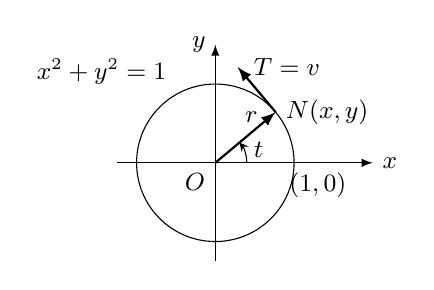
\begin{tikzpicture}[font=\small]
\draw[-latex](-1.25,0)--(2,0)node[right]{$x$};
\draw[-latex](0,-1.25)--(0,1.5)node[left]{$y$};
\draw(0,0) circle (1);
\draw[-latex,thick](0,0)node[below left]{$O$}--++(40:1)node[pos=0.6,above]{$\kvec{r}$}node[right]{$N(x,y)$};
\draw[-latex,thick](40:1)--++(130:0.75)node[right,xshift=0.5ex]{$\kvec{T}=\kvec{v}$};
\draw[-stealth]([shift={(0:0.4)}]0,0) arc (0:40:0.4)node[pos=0.6,right]{$t$};
\draw(1,0)node[below,xshift=2ex]{$(1,0)$};
\draw(120:1)node[above left]{$x^2+y^2=1$};
\end{tikzpicture}
\caption{حرکت \عددی{\kvec{r}(t)=(\cos t)\ai+(\sin t)\aj} برائے مثال \حوالہ{مثال_سمتی_تفاعل_اکائی_دائرہ_مماسی_سمتیہ}}
\label{شکل_مثال_سمتی_تفاعل_اکائی_دائرہ_مماسی_سمتیہ}
\end{figure}

\حصہء{سوالات}
\ابتدا{سوالات}
سوال \حوالہ{سوال_سمتی_تفاعل_لمبائی_قوس_الف} تا سوال \حوالہ{سوال_سمتی_تفاعل_لمبائی_قوس_ب} میں منحنی کا اکائی  مماسی سمتیہ تلاش کریں۔وقفہ پر منحنی کی لمبائی بھی دریافت کریں۔


\ابتدا{سوال}\شناخت{سوال_سمتی_تفاعل_لمبائی_قوس_الف}
$\kvec{r}(t)=(2\cos t)\ai+(2\sin t)\aj+\sqrt{5} t\ak,\quad 0\le t\le \pi$
\انتہا{سوال}  
%=========
\ابتدا{جواب}
\wf{\unexpanded{
$\kvec{T}=(-\tfrac{2}{3}\sin t)\ai+(\tfrac{2}{3}\cos t)\aj+\tfrac{\sqrt{5}}{3}\ak,\quad 3\pi$
}}
\انتہا{جواب}
%================
\ابتدا{سوال}
$\kvec{r}(t)=(6\sin 2t)\ai+(6\cos 2t)\aj+5t\ak,\quad 0\le t\le \pi$
\انتہا{سوال}
%=====================
\ابتدا{سوال}
$\kvec{r}(t)=t\ai+\tfrac{2}{3}t^{3/2}\ak,\quad 0\le t\le 8$
\انتہا{سوال}  
%=========
\ابتدا{جواب}
\wf{\unexpanded{
$\kvec{T}=\tfrac{1}{\sqrt{1+t}}\ai+\tfrac{\sqrt{t}}{\sqrt{1+t}}\ak,\quad \tfrac{52}{3}$
}}
\انتہا{جواب}
%=====================
\ابتدا{سوال}
$\kvec{r}(t)=(2+t)\ai-(t+1)\aj+t\ak,\quad 0\le t\le 3$
\انتہا{سوال}
%=====================
\ابتدا{سوال}
$\kvec{r}(t)=(\cos^3t)\aj+(\sin^3t)\ak,\quad 0\le t\le \pi/2$
\انتہا{سوال}  
%=========
\ابتدا{جواب}
\wf{\unexpanded{
$\kvec{T}=-\cos t\aj+\sin t\ak,\quad \tfrac{3}{2}$
}}
\انتہا{جواب}
%=====================
\ابتدا{سوال}
$\kvec{r}(t)=6t^3\ai-2t^3\aj-3t^3\ak,\quad 1\le t\le 2$
\انتہا{سوال}
%=====================
\ابتدا{سوال}
$\kvec{r}(t)=(t\cos t)\ai+(t\sin t)\aj+\tfrac{2\sqrt{2}}{3}t^{3/2}\ak,\quad 0\le t\le \pi$
\انتہا{سوال}  
%=========
\ابتدا{جواب}
\wf{\unexpanded{
$\kvec{T}=(\tfrac{\cos t-t\sin t}{t+1})\ai+(\tfrac{\sin t+t\cos t}{t+1})\aj+(\tfrac{\sqrt{2}t^{1/2}}{t+1})\ak,\quad \tfrac{\pi^2}{2}+\pi$
}}
\انتہا{جواب}
%=====================
\ابتدا{سوال}\شناخت{سوال_سمتی_تفاعل_لمبائی_قوس_ب}
$\kvec{r}(t)=(t\sin t+\cos t)\ai+(t\cos t-\sin t)\aj,\quad \sqrt{2}\le t\le 2$
\انتہا{سوال}
%=====================
\ابتدا{سوال}
مبدا سے   بڑھتی لمبائی کے رخ  درج ذیل منحنی پر مبدا سے \عددی{26\pi} دور نقطہ تلاش کریں۔
\begin{align*}
\kvec{r}(t)=(5\sin t)\ai+(5\cos t)\aj+12t\ak
\end{align*}
\انتہا{سوال}  
%=========
\ابتدا{جواب}
\wf{\unexpanded{
$(0,5,24\pi)$
}}
\انتہا{جواب}
%======================
\ابتدا{سوال}
مبدا سے   بڑھتی لمبائی کے مخالف رخ  درج ذیل منحنی پر مبدا سے \عددی{13\pi} دور نقطہ تلاش کریں۔
\begin{align*}
\kvec{r}(t)=(12\sin t)\ai-(12\cos t)\aj+5t\ak
\end{align*}
\انتہا{سوال}
%=====================
سوال \حوالہ{سوال_سمتی_تفاعل_مقدار_معلوم_لمبائی_قوس_الف} تا سوال \حوالہ{سوال_سمتی_تفاعل_مقدار_معلوم_لمبائی_قوس_ب}  میں \عددی{t=0} سے دور کسی نقطہ پر  مقدار معلوم لمبائی قوس درج ذیل تکمل کی قیمت حاصل کرتے ہوئے    تلاش کریں۔
\begin{align*}
s&=\int_0^t \abs{\kvec{v}(\tau)}\dif \tau&&\text{\RL{\small{مساوات \حوالہ{مساوات_سمتی_تفاعل_لمبائی_قوس_پ}}}}
\end{align*}
اس کے بعد دیے گئے وقفہ پر منحنی کی لمبائی تلاش کریں۔

\ابتدا{سوال}\شناخت{سوال_سمتی_تفاعل_مقدار_معلوم_لمبائی_قوس_الف}
$\kvec{r}(t)=(4\cos t)\ai+(4\sin t)\aj+3t\ak,\quad 0\le t\le \pi/2$
\انتہا{سوال}  
%=========
\ابتدا{جواب}
\wf{\unexpanded{
$s(t)=5t,\quad L=\tfrac{5\pi}{2}$
}}
\انتہا{جواب}
%===================
\ابتدا{سوال}
$\kvec{r}(t)=(\cos t+t\sin t)\ai+(\sin t-t\cos t)\aj,\quad \tfrac{\pi}{2}\le t\le \pi$
\انتہا{سوال}
%===================
\ابتدا{سوال}
$\kvec{r}(t)=(e^t\cos t)\ai+(e^t\sin t)\aj+e^t\ak,\quad -\ln 4\le t\le 0$
\انتہا{سوال}  
%=========
\ابتدا{جواب}
\wf{\unexpanded{
$s(t)=\sqrt{3}e^t-\sqrt{3},\quad L=\tfrac{3\sqrt{3}}{4}$
}}
\انتہا{جواب}
%===================
\ابتدا{سوال}\شناخت{سوال_سمتی_تفاعل_مقدار_معلوم_لمبائی_قوس_ب}
$\kvec{r}(t)=(1+2t)\ai+(1+3t)\aj+(6-6t)\ak,\quad -1\le t\le 0$
\انتہا{سوال}
%===================
\ابتدا{سوال}
نقطہ \عددی{(0,0,1)}  سے \عددی{(\sqrt{2},\sqrt{2},0)} تک درج  ذیل منحنی کی لمبائی تلاش کریں۔
\begin{align*}
\kvec{r}(t)=(\sqrt{2}t)\ai+(\sqrt{2}t)\aj+(1-t^2)\ak
\end{align*}
\انتہا{سوال}  
%=========
\ابتدا{جواب}
\wf{\unexpanded{
$\sqrt{2}+\ln(1+\sqrt{2})$
}}
\انتہا{جواب}
%=================
\ابتدا{سوال}
ہم نے مثال \حوالہ{مثال_سمتی_تفاعل_مقدار_معلوم_لمبائی_قوس_الف} میں پیچ دار منحنی کے ایک چکر کی لمبائی \عددی{2\pi\sqrt{2}} تلاش کی۔ ایک مربع جس  کا  ضلع \عددی{2\pi} ہو  کے وتر کی لمبائی بھی یہی ہو گی۔ دکھائیں کہ جس نلکی پر پیچ دار منحنی کا ایک چکر  لپٹا   گیا ہے، اس کو انتصابی کاٹ کر سیدھا کرنے سے یہی مربع حاصل ہو گا۔
\انتہا{سوال}
%================
\ابتدا{سوال}
\begin{enumerate}[a.]
\item
دکھائیں کہ  \عددی{\kvec{r}(t)=(\cos t)\ai+(\sin t)\aj+(1-\cos t)\ak,\, 0\le t\le 2\pi} ایک ترخیم ہے۔  ایسا کرنے کی خاطر دکھائیں کہ  \عددی{\kvec{r}}   قائمہ دائری نلکی اور  ایک مستوی کا مطقاطع  ہے۔ ان قائمہ دائری نلکی اور مستوی  کی مساواتیں تلاش کریں۔
\item
نلکی پر ترخیم کا خاکہ کھینچیں اور اس پر     نقاط \عددی{t=0}، \عددی{t=\tfrac{\pi}{2}}، \عددی{t=\pi} اور \عددی{t=\tfrac{3\pi}{2}} پر  اکائی مماسی سمتیات بنائیں۔ 
\item
دکھائیں کہ سمتیہ اسراع ہر صورت مستوی کو متوازی ہو گا (مستوی کے عمودی سمتیہ کو قائمہ ہو گا)۔یوں اگر  آپ اسراع کو ترخیم کے ساتھ جڑا دکھائیں تب یہ ترخیم کے مستوی میں پایا جائے گا۔ نقاط \عددی{t=0}، \عددی{t=\tfrac{\pi}{2}}، \عددی{t=\pi} اور \عددی{t=\tfrac{3\pi}{2}} پر سمتیات اسراع  کو خاکہ میں شامل کریں۔
\item
ترخیم کی لمبائی کا تکمل لکھیں۔اس تکمل کی قیمت تلاش کرنے کی کوشش نہ کریں چونکہ یہ ایک غیر بنیادی تکمل ہے۔
\item
اعدادی ترکیبات سے ترخیم کی لمبائی دو  اعشاریہ درست  معلوم کریں۔
\end{enumerate}
\انتہا{سوال}  
%=========
\ابتدا{جواب}
\wf{\unexpanded{
ا) نلکی \عددی{x^2+y^2=1} اور مستوی \عددی{x+z=1}\\
د) \عددی{L=\int_0^{2\pi}\sqrt{1+\sin^2t}\dif t}\\
  ہ) \عددی{L\approx 7.64} 
}}
\انتہا{جواب}

%================
\ابتدا{سوال}\ترچھا{لمبائی کی قیمت مقدار معلوم روپ  پر منحصر نہیں ہے۔}\\
یہ دکھانے کی خاطر کہ لمبائی کی قیمت مقدار معلوم روپ پر منحصر نہیں ہے، ہم  پیچ دار منحنی کے ایک چکر کی لمبائی درج  ذیل ( مختلف) مقدار معلوم مساواتیں استعمال کرتے ہوئے حاصل کرتے ہیں۔
\begin{enumerate}[a.]
\item
$\kvec{r}(t)=(\cos 4t)\ai+(\sin 4t)\aj+4t\ak,\quad 0\le t\le \tfrac{\pi}{2}$
\item
$\kvec{r}(t)=(\cos (t/2))\ai+(\sin (t/2))\aj+(t/2)\ak,\quad 0\le t\le 4\pi$
\item
$\kvec{r}(t)=(\cos t)\ai-(\sin t)\aj-t\ak,\quad -2\pi \le t\le 0$
\end{enumerate}
\انتہا{سوال}
%===========
\انتہا{سوالات}

%%%%%%%%%%%%%%%%%%%%%

\حصہ{انحنا، مروڑ اور \عددی{TNB} چھوکٹ}
اس حصہ میں ہم   تین آپس میں عمودی اکائی سمتیات پر مبنی ایسا چھوکٹ متعارف کرتے ہیں جو  فضا میں منحنی پر جسم کے ساتھ ساتھ چلتا ہو (شکل \حوالہ{شکل_سمتی_تفاعل_چھوکٹ}) ۔ اس چھوکٹ کے تین سمتیات  ہیں۔ پہلا  اکائی مماسی سمتیہ \عددی{\kvec{T}} ہے۔ دوسرا \عددی{\kvec{N}} ہے جو  \عددی{\tfrac{\dif \kvec{R}}{\dif s}} کے رخ اکائی سمتیہ ہے۔تیسرا اکائی سمتیہ  \عددی{\kvec{B}=\kvec{T}\times\kvec{N}} ہے ۔ یہ سمتیات اور ان کے تفرقات  اگر معلوم ہوں، فضا  میں سواری  کی  سمت بندی اور اس کی راہ  میں موڑ  اور بل  کے بارے میں مفید معلومات   مہیا کرتے ہیں۔

مثال کے طور پر  \عددی{\abs{\tfrac{\dif \kvec{R}}{\dif s}}} ہمیں بتاتا ہے  کہ راہ پر  آگے چلتے ہوئے، سواری  کی   راہ کتنی  دائیں یا بائیں  مڑتی  ہے؛ اسی لئے اس کو سواری کی راہ کی\اصطلاح{ انحنا}\فرہنگ{انحنا}\حاشیہب{curvature}\فرہنگ{curvature} کہتے ہیں۔ عدد \عددی{-(\dif \kvec{B}/\dif s)\cdot\kvec{N}} ہمیں بتاتا ہے کہ راہ پر آگے چلتے ہوئے،  سواری کی راہ مستوی حرکت سے کتنی باہر مڑتی ہے یا بل کھاتی ہے؛ اس کو سواری کی راہ کی \اصطلاح{مروڑ}\فرہنگ{مروڑ}\حاشیہب{torsion}\فرہنگ{torsion} کہتے ہیں۔ دوبارہ شکل \حوالہ{شکل_سمتی_تفاعل_چھوکٹ} پر نظر ڈالیں۔ اگر    قوسی راہ پر ایک  ریل گاڑی،   \عددی{P}،   اوپر    چڑھ رہی ہو تب فی اکائی فاصلہ اس   کی   سر بتی جتنی دائیں یا بائیں مڑتی ہو، یہ اس کی انحنا ہو گی۔سمتیات \عددی{\kvec{T}} اور \عددی{\kvec{N}} کے  مستوی سے ریل گاڑی  کا انجن  جس شرح سے باہر  نکلتا  ہو، یہ اس کی مروڑ ہو گی۔ 
\begin{figure}
\centering
\begin{minipage}{0.45\textwidth}
\centering
\pgfmathsetmacro{\ang}{20}
\pgfmathsetmacro{\kang}{20}
\pgfmathsetmacro{\s}{-120}
\pgfmathsetmacro{\e}{65}
\pgfmathsetmacro{\a}{2}
\pgfmathsetmacro{\b}{1.3}
\pgfmathsetmacro{\ka}{2.5}
\pgfmathsetmacro{\kb}{0.5}
\begin{tikzpicture}[font=\small,declare function={fp(\x)=(\x/\a)^2;fn(\x)=(\x/(1.2*\a))^2;}]
\draw[rotate=\ang](0,0) circle (\a cm and \b cm);
\draw[rotate=\ang,->-=0.9,domain=0:\a] plot (\x,{fp(\x)});
\draw[rotate=\ang,domain=0:1.2*\a] plot (-\x,{fn(\x)});
\draw[rotate=\ang](-0.9*1.2*\a,{(fn(0.9*1.2*\a)})++(0,0.1)--++(-90-\ang:0.2)node[below,xshift=-1ex]{$s=0$};
\draw[-latex,thick](0,0)node[below,xshift=-0.5ex]{$P$}--++(\ang:\a)node[pos=0.75,below]{$\kvec{T}$};
\draw[-latex,thick](0,0)--++(90+\ang:\b)node[pos=0.4,left]{$\kvec{N}$};
\draw[rotate=90]([shift={(\s:\ka cm and \kb cm)}]0,0) arc (\s:\e:\ka cm and \kb cm);
\draw(0,0)--++(-90+\ang:\b);
\draw[-latex,thick](0,0)--++(0,\ka)node[pos=0.7,xshift=-1.25ex]{$\kvec{B}$};
\draw[-latex,thick,gray](\ang:\a)--++(90+\ang:0.75)node[pos=0.5,pin={[black,align=center,pin edge=-]45:{\RL{\عددی{P} پر انحنا}\\  $\abs{\dif\kvec{T}/\dif s}$}}]{};
\draw[-latex,thick,gray](0,\ka)--++(90+\ang:0.5)node[right,black]{$\tfrac{\dif \kvec{B}}{\dif s}$};
\draw(90+\ang:2)node[left,align=center]{\RL{\عددی{P} پر مروڑ}\\  $-(\tfrac{\dif \kvec{B}}{\dif s})\cdot \kvec{N}$};
\end{tikzpicture}
\caption{ہر متحرک جسم کے ساتھ  ایک \عددی{\kvec{}}TNB چھوکٹ سفر کرتا ہے جو اس کی راہ کا کردار بیان کرتا ہے۔}
\label{شکل_سمتی_تفاعل_چھوکٹ}
\end{minipage}\hfill
\begin{minipage}{0.45\textwidth}
\centering
\begin{tikzpicture}[font=\small,declare function={f(\x)=0.6+(\x/3)^2;}]
\pgfmathsetmacro{\a}{20}
\draw[-latex](0,0)--(3,0)node[right]{$x$};
\draw[-latex](0,0)--(0,2)node[left]{$y$};
\draw[->-=0.25,domain=0.2:3]plot ({\x},{f(\x)});
\draw(0.3,{f(0.3)})++(0,0.1)--++(0,-0.2)node[below]{$P_0$};
\draw[-latex](1.5,{f(1.5)})node[circ]{}node[above]{$P$}--++(\a:1.25)node[pos=0.75,below]{$\kvec{T}$};
\draw(1,{f(1)})node[below]{$s$};
\end{tikzpicture}
\caption{بڑھتی لمبائی قوس کے رخ چلتے ہوئے اکائی مماسی سمتیہ \عددی{\kvec{T}} مڑتا ہے۔نقطہ \عددی{P} پر \عددی{\abs{\dif \kvec{T}/\dif s}} کی قیمت کو \عددی{P} پر منحنی کی انحنا کہتے ہیں۔}
\label{شکل_سمتی_تفاعل_ریل_گاڑی}
\end{minipage}
\end{figure}

\جزوحصہء{مستوی منحنی کی انحنا}
جیسے جیسے ایک ذرہ مستوی منحنی  میں حرکت کرتا ہے، منحنی کے مڑنے سے  \عددی{\kvec{T}=\tfrac{\dif \kvec{r}}{\dif s}} بھی مڑتا ہے۔ چونکہ \عددی{\kvec{T}} اکائی سمتیہ ہے لہٰذا اس کی لمبائی تبدیل نہیں ہوتی  اور راہ پر چلتے ہوئے  صرف اس کا رخ تبدیل ہوتا ہے۔ منحنی پر چلتے ہوئے اکائی فاصلہ پر \عددی{\kvec{T}}   کی شرح تبدیلی کو انحنا کہتے ہیں (شکل \حوالہ{شکل_سمتی_تفاعل_ریل_گاڑی})۔ انحنا کو روایتی طور پر یونانی حرف  \عددی{\kappa} (کاہپا) سے ظاہر کیا جاتا ہے۔

\ابتدا{تعریف}
 ایک  ہموار منحنی جس  کا اکائی مماسی سمتیہ \عددی{\kvec{T}}  ہو، کا تفاعل انحنا درج ذیل ہو گا۔
\begin{align*}
\kappa=\abs{\frac{\dif \kvec{T}}{\dif s}}
\end{align*}
\انتہا{تعریف}
%==========

اگر \عددی{\abs{\dif\kvec{T}/\dif s}} بڑی قیمت ہو تب نقطہ \عددی{P} سے گزرتے ہوئے ذرہ بہت تیزی سے مڑے گا اور \عددی{P} پر انحنا زیادہ ہو گی۔ اگر \عددی{\abs{\dif\kvec{T}/\dif s}} صفر کے قریب ہو تب \عددی{\kvec{T}} کا رخ آہستہ تبدیل ہو گا اور \عددی{P} پر انحنا کم ہو گی۔ اس تعریف کو  پرکھتے ہوئے  ہم درج ذیل دو مثالوں میں دیکھتے ہیں کہ سیدھے خط اور دائروں کی انحنا  مستقل ہو گی۔

\ابتدا{مثال}\ترچھا{سیدھے لکیر کی انحنا صفر ہو گی}\\
سیدھے لکیر پر اکائی مماسی سمتیہ \عددی{\kvec{T}}  کا رخ تبدیل نہیں ہوتا ہے لہٰذا اس کے اجزاء مستقل ہوں گے۔یوں \عددی{\abs{\dif\kvec{T}/\dif s}=\abs{\kvec{0}}=0} ہو گا (شکل \حوالہ{شکل_مثال_سمتی_تفاعل_سیدھی_لکیر_مماسی_سمتیہ})۔
\انتہا{مثال}
%================= 
\ابتدا{مثال}\شناخت{مثال_سمتی_تفاعل_دائرہ_انحنا}\ترچھا{رداس \عددی{a} کے دائرے کی انحنا \عددی{\tfrac{1}{a}} ہو گی}\\
ہم دائرہ کی مقدار معلوم مساوات
\begin{align*}
\kvec{r}(\theta)=(a\cos\theta)\ai+(a\sin\theta)\aj
\end{align*}
میں \عددی{\theta=\tfrac{s}{a}} پر کر کے اس کی لمبائی قوس \عددی{s} کے لحاض سے مقدار معلوم روپ حاصل کرتے ہیں (شکل \حوالہ{شکل_مثال_سمتی_تفاعل_دائرہ_انحنا})۔
\begin{align*}
\kvec{r}=(a\cos\frac{s}{a})\ai+(a\sin\frac{s}{a})\aj
\end{align*}
یوں
\begin{align*}
\kvec{T}=\frac{\dif\kvec{r}}{\dif s}=(-\sin\frac{s}{a})\ai+(\cos\frac{s}{a})\aj
\end{align*}
اور
\begin{align*}
\frac{\dif \kvec{T}}{\dif s}=(-\frac{1}{a}\cos\frac{s}{a})\ai-(\frac{1}{a}\sin\frac{s}{a})\aj
\end{align*}
ہوں گے۔اس طرح کسی بھی \عددی{س} کے لئے درج ذیل ہو گا۔
\begin{align*}
\kappa&=\abs{\frac{\dif \kvec{T}}{\dif s}}\\
&=\sqrt{\frac{1}{a^2}\cos^2\frac{s}{a}+\frac{1}{a^2}\sin^2\frac{s}{a}}\\
&=\frac{1}{\sqrt{a^2}}=\frac{1}{\abs{a}}=\frac{1}{a}\quad\quad \text{\small\RL{\عددی{a>0} کی بنا \عددی{\abs{a}=a} ہو گا}}
\end{align*}
\انتہا{مثال}
%================
\begin{figure}
\centering
\begin{minipage}{0.45\textwidth}
\centering
\begin{tikzpicture}
\pgfmathsetmacro{\a}{20}
\pgfmathsetmacro{\b}{1}
\draw[](0,0)--++(\a:0.25*\b);
\draw[->-=0.5](\a:0.25*\b)node[circ]{}--++(\a:\b)node[pos=0.5,below]{$\kvec{T}$};
\draw[->-=0.5](0,0)++(\a:1.25*\b)node[circ]{}--++(\a:\b);
\draw[->-=0.5](0,0)++(\a:2.25*\b)node[circ]{}--++(\a:\b);
\end{tikzpicture}
\caption{سیدھے لکیر پر \عددی{\kvec{T}} کا رخ تبدیل نہیں ہوتا ہے لہٰذا اس کی انحنا \عددی{\abs{\dif\kvec{T}/\dif s}} صفر ہو گی۔}
\label{شکل_مثال_سمتی_تفاعل_سیدھی_لکیر_مماسی_سمتیہ}
\end{minipage}\hfill
\begin{minipage}{0.45\textwidth}
\centering
\begin{tikzpicture}
\draw[-latex](0,0)--(2,0)node[right]{$x$};
\draw[-latex](0,0)--(0,1.5)node[left]{$y$};
\draw(0,0)node[left]{$O$} circle (1.25);
\draw(0,0)--++(45:1.25)node[circ]{}node[right,yshift=1ex]{$P(a\cos\tfrac{s}{a},a\sin\tfrac{s}{a})$}node[pos=0.7,shift={(90+45:1ex)}]{$a$};
\draw[-stealth]([shift={(0:0.5)}]0,0) arc (0:45:0.5)node[pos=0.6,right]{$\theta$};
\draw(1.25,0)node[circ]{}node[pin={[align=center]-45:{\RL{بنیاد}}\\  $(a,0)$}]{};
\draw[thick]([shift={(0:1.25)}]0,0) arc (0:45:1.25)node[pos=0.5,right]{$s=a\theta$};
\end{tikzpicture}
\caption{دائرہ برائے مثال \حوالہ{مثال_سمتی_تفاعل_دائرہ_انحنا}}
\label{شکل_مثال_سمتی_تفاعل_دائرہ_انحنا}
\end{minipage}
\end{figure}

\جزوحصہء{صدر  اکائی عمودی سمتیہ}
چونکہ \عددی{\kvec{T}} کی لمبائی اکائی ہے لہٰذا \عددی{\tfrac{\dif \kvec{T}}{\dif s}} اور \عددی{\kvec{T}} آپس میں عمودی ہوں گے (حصہ \حوالہ{حصہ_سمتی_تفاعل_سمتی_قیمت_تفاعل_اور_فضائی_منحنیات})۔ یوں \عددی{\tfrac{\dif\kvec{T}}{\dif s}} کو لمبائی \عددی{\kappa} سے تقسیم کرنے سے ایسا اکائی  سمتیہ حاصل ہو گا جو   \عددی{\kvec{T}} کو عمودی  ہو گا (شکل \حوالہ{شکل_سمتی_تفاعل_اکائی_مماسی_اور_عمودی_سمتیات})۔ 
\begin{figure}
\centering
\pgfmathsetmacro{\a}{0}
\pgfmathsetmacro{\b}{1.5}
\pgfmathsetmacro{\c}{2.75}
\pgfmathsetmacro{\d}{0.65}
\pgfmathsetmacro{\e}{2.3}
\begin{tikzpicture}[scale=1.5,font=\small,declare function={f(\x)=(\x-\a)*(\x-\b)*(\x-\c);df(\x)=3*\x^2-2*(\b+\c)*\x+\b*\c;}]
\draw[->-=0.2,domain=-0.1:3,smooth]plot ({\x},{f(\x)});
\draw(0.1,{f(0.1)})++(-10:0.1)--++(170:0.2)node[left]{$P_0$};
\draw(0.21,{f(0.21)})node[left]{$s$};
\draw[-latex](\d,{f(\d)})node[circ]{}node[above]{$P_1$}--++(1,{df(\d)})node[above]{$\kvec{T}$};
\draw[-latex](\d,{f(\d)})--++({df(\d)},-1)node[below,xshift=1ex]{$\kvec{N}=\frac{1}{\kappa}\frac{\dif \kvec{T}}{\dif s}$};
\draw[-latex](\e,{f(\e)})node[circ]{}node[below]{$P_2$}--++(1,{df(\e)})node[above]{$\kvec{T}$};
\draw[-latex](\e,{f(\e)})--++({-df(\e)},1)node[above,xshift=1ex]{$\kvec{N}=\frac{1}{\kappa}\frac{\dif\kvec{T}}{\dif s}$};
\end{tikzpicture}
\caption{منحنی کا عمودی سمتیہ \عددی{\tfrac{\dif\kvec{T}}{\dif s}} ہر وقت اس رخ ہوتا ہے جس رخ \عددی{\kvec{T}} مڑتا ہو۔ سمتیہ \عددی{\kvec{N}} کا رخ سمتیہ \عددی{\tfrac{\dif\kvec{T}}{\dif s}} کا رخ ہے۔}
\label{شکل_سمتی_تفاعل_اکائی_مماسی_اور_عمودی_سمتیات}
\end{figure}
\ابتدا{تعریف}
جس نقطہ پر \عددی{\kappa\ne 0} ہو وہاں مستوی میں منحنی کا صدر اکائی سمتیہ \عددی{\kvec{N}}  درج ذیل ہو گا۔
\begin{align*}
\kvec{N}=\frac{1}{\kappa}\frac{\dif\kvec{T}}{\dif s}
\end{align*} 
\انتہا{تعریف}
%===========

موڑ پر سمتیہ \عددی{\tfrac{\dif\kvec{T}}{\dif s}} کا رخ اس جانب ہو گا جس جانب منحنی مڑتی ہو۔یوں اگر بڑھتے فاصلہ کے رخ منہ کرتے ہوئے، اگر \عددی{\kvec{T}}  گھڑی کے رخ مڑے   تب سمتیہ  \عددی{\tfrac{\dif\kvec{T}}{\dif s}}  کا رخ دائیں  ہو گا اور اگر \عددی{\kvec{T}}  گھڑی کے مخالف رخ مڑتی ہو تب اس کا رخ بائیں ہو گا۔  دوسرے لفظوں میں صدر عمودی سمتیہ \عددی{\kvec{N}}منحنی کے   مقعر  رخ ہو گا (شکل \حوالہ{شکل_سمتی_تفاعل_اکائی_مماسی_اور_عمودی_سمتیات})۔  جس  نقطہ پر  \عددی{\kappa=0} ہو، وہاں کے بارے میں سوال \حوالہ{سوال_سمتی_تفاعل_اکائی_این}  میں غور کیا گیا ہے۔


 تعریف کی رو سے  منحنی \عددی{\kvec{r}(t)=f(t)\ai+g(t)\aj}  کی لمبائی قوس،   مثبت \عددی{\tfrac{\dif s}{\dif t}} کے لئے ہو گی لہٰذا \عددی{\tfrac{\dif s}{\dif t}=\abs{\tfrac{\dif s}{\dif t}}} ہو گا   اور زنجیری قاعدہ درج ذیل دے گا۔
\begin{align}
\kvec{N}&=\frac{\dif\kvec{T}/\dif s}{\abs{\dif\kvec{T}/\dif s}}\nonumber\\
&=\frac{(\dif\kvec{T}/\dif t)(\dif t/\dif s)}{\abs{\dif\kvec{T}/\dif t}\abs{\dif t/\dif s}}\nonumber\\
&=\frac{\dif\kvec{T}/\dif t}{\abs{\dif\kvec{T}/\dif t}}
\end{align}

اس طرح ہم \عددی{\kappa} اور \عددی{s} حاصل کیے بغیر \عددی{\kvec{N}} حاصل کر سکتے ہیں۔


\ابتدا{مثال}
درج ذیل دائری حرکت کے لئے \عددی{\kvec{T}} اور \عددی{\kvec{N}} تلاش کریں۔
\begin{align*}
\kvec{r}(t)=(\cos 2t)\ai+(\sin 2t)\aj
\end{align*}
حل:\quad
ہم پہلے \عددی{\kvec{T}} دریافت کرتے ہیں۔
\begin{align*}
\kvec{v}&=-(2\sin 2t)\ai+(2\cos 2t)\aj,\\
\abs{\kvec{v}}&=\sqrt{4\sin^22t+4\cos^22t}=2,\\
\kvec{T}&=\frac{\kvec{v}}{\abs{\kvec{v}}}\\
&=-(\sin 2t)\ai+(\cos 2t)\aj
\end{align*}
یوں
\begin{align*}
\frac{\dif \kvec{T}}{\dif t}&=-(2\cos 2t)\ai-(2\sin 2t)\aj,\\
\abs{\frac{\dif \kvec{T}}{\dif t}}&=\sqrt{4\cos^22t+4\sin^22t}=2
\end{align*}
اور درج ذیل ہو گا۔
\begin{align*}
\kvec{N}&=\frac{\dif \kvec{T}/\dif t}{\abs{\dif\kvec{T}/\dif t}}\\
&=-(\cos 2t)\ai-(\sin 2t)\aj
\end{align*}
\انتہا{مثال}
%===============

\حصہء{انحنا کا دائرہ اور انحنا کا رداس}
مستوی منحنی پر نقطہ \عددی{P}  جہاں \عددی{\kappa\ne 0} ہو،  \اصطلاح{دائرہ انحنا}\فرہنگ{دائرہ!انحنا}\حاشیہب{circle of curvature}\فرہنگ{circle!of curvature} سے مراد  اس مستوی میں وہ دائرہ ہے جو درج ذیل کو مطمئن کرتا ہو۔
\begin{enumerate}[a.]
\item
نقطہ \عددی{P} پر یہ منحنی کا مماسی ہو (منحنی کا مماسی خط ہی اس کا مماسی خط ہے)؛
\item
نقطہ \عددی{P} پر اس کی انحنا اور منحنی کی انحنا ایک دوسرے کے برابر ہوں ؛
\item
یہ منحنی کے اندرونی یعنی مقعر رخ  پایا جائے (شکل \حوالہ{شکل_سمتی_تفاعل_دائرہ_انحنا})۔
\end{enumerate}

\begin{figure}
\centering
\begin{minipage}{0.45\textwidth}
\centering
\begin{tikzpicture}
\pgfmathsetmacro{\r}{1.5}
\pgfmathsetmacro{\ang}{-30}
\draw(0,0) circle (\r);
\draw[](0,0)node[circ]{}node[above,align=center]{\RL{انحنا کا}\\   \RL{مرکز}}--++(\ang:\r)node[right,yshift=-1ex]{$P(x,y)$}node[pos=0.75,above,yshift=0.5ex,align=center]{\RL{انحنا کا}\\  \RL{رداس}};
\draw[-latex,thick](\ang:\r)--++(180+\ang:1)node[below,pos=0.5,xshift=-0.5ex]{$\kvec{N}$};
\draw[-latex,thick](\ang:\r)--++(\ang+90:1)node[right,pos=0.75]{$\kvec{T}$};
\draw(\ang:\r) to [out=\ang+90,in=-90]++(0.5,2)node[right]{منحنی};
\draw(\ang:\r) to [out=\ang-90,in=-60](-1,0.5);
\end{tikzpicture}
\caption{نقطہ \عددی{P(x,y)} پر دائرہ انحنا منحنی کے اندرونی رخ ہو گا۔}
\label{شکل_سمتی_تفاعل_دائرہ_انحنا}
\end{minipage}\hfill
\begin{minipage}{0.45\textwidth}
\centering
\begin{tikzpicture}[font=\small,declare function={fx(\ra,\t)=\ra*cos(\t);fy(\rb,\t)=\rb*sin(\t);fz(\rc,\t)=\rc*\t;}]
\pgfmathsetmacro{\h}{2.25}
\pgfmathsetmacro{\ra}{2}
\pgfmathsetmacro{\rb}{0.25*\ra}
\pgfmathsetmacro{\rc}{2/470}
\pgfmathsetmacro{\ta}{-110}
\pgfmathsetmacro{\tb}{0}
\pgfmathsetmacro{\tc}{180}
\pgfmathsetmacro{\td}{360}
\pgfmathsetmacro{\te}{-20}
\pgfmathsetmacro{\tf}{360+\ta}
\draw[-latex](0,0)--++(-145:2)node[left]{$x$};
\draw[-latex](0,0)--++(0:2.5)node[right]{$y$};
\draw[-latex](0,0)--++(0,3)node[left]{$z$};
 \draw[-latex](0,0,0)node[left,yshift=1ex]{$O$}--({fx(\ra,\te)},{fz(\rc,\te-\ta)+fy(\rb,\te)})node[circ]{}node[pos=0.4,above]{$\kvec{r}$}node[right]{$P$};
\draw[dashed,domain=40:180,variable=\t]plot ({fx(\ra,\t)},{fy(\rb,\t)});
\draw[domain=180:360,variable=\t]plot ({fx(\ra,\t)},{fy(\rb,\t)});
\draw[domain=0:360,variable=\t]plot ({fx(\ra,\t)},{\h+fy(\rb,\t)});
\draw  ({fx(\ra,300)},{fy(\rb,300)})node[below,yshift=-1ex]{$x^2+y^2=a^2$};
\draw(-\ra,0)--++(0,\h);
\draw(\ra,0)--++(0,\h);
\draw[domain=\ta:\tb,variable=\t]plot ({fx(\ra,\t)},{fz(\rc,\t-\ta)+fy(\rb,\t)});
\draw[dashed,domain=\tb:\tc,variable=\t]plot ({fx(\ra,\t)},{fz(\rc,\t-\ta)+fy(\rb,\t)});
\draw[domain=\tc:\td,variable=\t]plot ({fx(\ra,\t)},{fz(\rc,\t-\ta)+fy(\rb,\t)});
\draw  ({fx(\ra,\ta)},{fz(\rc,\ta-\ta)+fy(\rb,\ta)})node[circ]{}node[below,xshift=1ex]{$t=0$}node[left,xshift=-2ex,yshift=-1ex]{$(a,0,0)$};
\draw  ({fx(\ra,\tb)},{fz(\rc,\tb-\ta)+fy(\rb,\tb)})node[circ]{}node[right,yshift=1ex]{$t=\frac{\pi}{2}$};
\draw  ({fx(\ra,\tf)},{fz(\rc,\tf-\ta)+fy(\rb,\tf)})node[circ]{}node[below]{$t=2\pi$};
\draw[dashed] ({fx(\ra,\tf)},{fz(\rc,\tf-\ta)+fy(\rb,\tf)})-- (0,{fz(\rc,\tf-\ta)})node[circ]{}node[right]{$2\pi b$};
\end{tikzpicture}
\caption{مثبت \عددی{a}، \عددی{b} کے لئے \عددی{\kvec{r}(t)=(a\cos t)\ai+(a\sin t)\aj}}
\label{شکل_مثال_سمتی_تفاعل_پیچ_دار_مثبت_الف_ب}
\end{minipage}
\end{figure}

نقطہ \عددی{P} پر منحنی کے \اصطلاح{ رداس انحنا}\فرہنگ{رداس!انحنا}\حاشیہب{radius of curvature}\فرہنگ{radius!of curvature}  سے مراد اس نقطہ پر دائرہ انحنا کا رداس ہے، جو مثال \حوالہ{مثال_سمتی_تفاعل_دائرہ_انحنا} کے مطابق درج ذیل ہو گا۔
\begin{align}
\text{\RL{رداس انحنا}}=\rho=\frac{1}{\kappa}
\end{align}
رداس انحنا جاننے کے لئے ہم \عددی{\kappa} معلوم کر کے اس کا  بالعکس متناسب  لیتے ہیں۔ نقطہ \عددی{P} پر  \اصطلاح{مرکز انحنا}\فرہنگ{مرکز!انحنا}\حاشیہب{center of curvature}\فرہنگ{center!of curvature} سے مراد  یہاں کے دائرہ انحنا کا مرکز ہو گا۔

\حصہء{فضائی منحنیات کی انحنا اور  عمودی سمتیات}
مستوی منحنیات کی طرح  فضا میں ہموار منحنی کے لئے مقدار معلوم لمبائی قوس  \عددی{s}،   مماسی اکائی سمتیہ \عددی{\kvec{T}} دیتا ہے۔ ہم اب بھی انحنا سے مراد 
\begin{align}\label{مساوات_سمتی_تفاعل_فضائی_انحنا}
\kappa=\abs{\frac{\dif \kvec{T}}{\dif s}}
\end{align}
لیتے ہیں۔ سمتیہ \عددی{\tfrac{\dif\kvec{T}}{\dif s}}  سمتیہ \عددی{\kvec{T}} کو عمودی ہو گا  اور ہم صدر اکائی عمودی سمتیہ سے مراد درج ذیل لیتے ہیں۔
\begin{align}\label{مساوات_سمتی_تفاعل_فضائی_اکائی_عمودی_سمتیہ}
\kvec{N}=\frac{1}{\kappa}\frac{\dif\kvec{T}}{\dif s}=\frac{\dif\kvec{T}/\dif t}{\abs{\dif\kvec{T}/\dif t}}
\end{align}

\ابتدا{مثال}\شناخت{مثال_سمتی_تفاعل_پیچ_دار_مثبت_الف_ب}
درج ذیل پیچ دار منحنی کی انحنا دریافت کریں (شکل \حوالہ{شکل_مثال_سمتی_تفاعل_پیچ_دار_مثبت_الف_ب})۔
\begin{align*}
\kvec{r}(t)=(a\cos t)\ai+(a\sin t)\aj+bt\ak,\quad a,b\ge 0,\, a^2+b^2\ne 0
\end{align*}
حل:\quad
ہم سمتی رفتار \عددی{\kvec{v}} سے \عددی{\kvec{T}} حاصل کرتے ہیں۔
\begin{align*}
\kvec{v}(t)&=-(a\sin t)\ai+(a\cos t)\aj+b\ak\\
\abs{\kvec{v}}&=\sqrt{a^2\sin^2t+a^2\cos^2t+b^2}=\sqrt{a^2+b^2}\\
\kvec{T}&=\frac{\kvec{v}}{\abs{\kvec{v}}}=\frac{1}{\sqrt{a^2+b^2}}[-(a\sin t)\ai+(a\cos t)\aj+b\ak]
\end{align*}
اب زنجیری قاعدہ سے \عددی{\tfrac{\dif \kvec{T}}{\dif s}} حاصل کرتے ہیں۔
\begin{align*}
\frac{\dif \kvec{T}}{\dif s}&=\frac{\dif \kvec{T}}{\dif t}\frac{\dif t}{\dif s}&&\text{\RL{\small{زنجیری قاعدہ}}}\\
&=\frac{\dif\kvec{T}}{\dif t}\cdot\frac{1}{\abs{\kvec{v}}}&&\frac{\dif s}{\dif t}=\abs{\kvec{v}}\implies \frac{\dif t}{\dif s}=\frac{1}{\abs{\kvec{v}}}\\
&=\frac{1}{\sqrt{a^2+b^2}}[-(a\cos t)\ai-(a\sin t)\aj]\cdot\big(\frac{1}{\sqrt{a^2+b^2}}\big)\\
&=\frac{a}{a^2+b^2}[-(\cos t)\ai-(\sin t)\aj]
\end{align*}
اس طرح درج ذیل ہو گا۔
\begin{align}
\kappa&=\abs{\frac{\dif \kvec{T}}{\dif s}}\nonumber\\
&=\frac{a}{a^2+b^2}\abs{-(\cos t)\ai-(\sin t)\aj}\nonumber\\
&=\frac{a}{a^2+b^2}\sqrt{(\cos t)^2+(\sin t)^2}=\frac{a}{a^2+b^2}\label{مساوات_مثال_انحنا}
\end{align}
ہم مساوات \حوالہ{مساوات_مثال_انحنا} سے دیکھتے ہیں کہ مستقل \عددی{a} کے لئے \عددی{b} بڑھانے سے انحنا کم ہوتی ہے۔ مستقل \عددی{b} کے لئے \عددی{a} کم کرنے  سے بھی  انحنا  آخر کار انحنا کم کرتی ہے۔ ایک اسپرنگ کھینچنے سے سیدھا ہوتا  ہے۔ 

اگر \عددی{b=0} ہو  تب پیچ دار  منحنی ایک دائرہ ہو گا جس کا رداس \عددی{a}  اور انحنا \عددی{\tfrac{1}{a}} ہو گی۔ اگر \عددی{a=0} ہو تب پیچ دار منحنی،  محور \عددی{z} پر سیدھا خط ہو گا اور اس کی انحنا \عددی{0} ہو گی۔
\انتہا{مثال}
%=================

\ابتدا{مثال}
گزشتہ مثال میں منحنی کے لئے  \عددی{\kvec{N}} تلاش کریں۔

حل:\quad
\begin{align*}
\frac{\dif \kvec{T}}{\dif t}&=-\frac{1}{\sqrt{a^2+b^2}}[(a\cos t)\ai+(a\sin t)\aj]&&\text{\RL{مثال \حوالہ{مثال_سمتی_تفاعل_پیچ_دار_مثبت_الف_ب}}}\\
\abs{\frac{\dif \kvec{T}}{\dif t}}&=\frac{1}{\sqrt{a^2+b^2}}\sqrt{a^2\cos^2t+a^2\sin^2t}=\frac{a}{\sqrt{a^2+b^2}}\\
\kvec{N}&=\frac{\dif \kvec{T}/\dif t}{\abs{\dif\kvec{T}/\dif t}}&&\text{\RL{مساوات \حوالہ{مساوات_سمتی_تفاعل_فضائی_اکائی_عمودی_سمتیہ}}}\\
&=-\frac{\sqrt{a^2+b^2}}{a}\cdot\frac{1}{\sqrt{a^2+b^2}}[(a\cos t)\ai+(a\sin t)\aj]\\
&=-(\cos t)\ai-(\sin t)\aj
\end{align*}
\انتہا{مثال}
%===================

\جزوحصہء{مروڑ اور  دوہری  عمودی سمتیہ}
فضا میں منحنی کا  \اصطلاح{دوہری عمودی سمتیہ}\فرہنگ{سمتیہ!دوہری عمودی}\حاشیہب{binormal vector}\فرہنگ{vector!binormal} \عددی{\kvec{B}=\kvec{T}\times\kvec{N}} ہے جو \عددی{\kvec{T}} اور \عددی{\kvec{N}} دونوں کو عمودی ہو گا  (شکل \حوالہ{شکل_سمتی_تفاعل_اکائی_عمودی_سمتیات_چھوکٹ})۔ سمتیات \عددی{\kvec{T}}، \عددی{\kvec{N}} اور \عددی{\kvec{B}} مل  کر دایاں ہاتھ، متحرک،  سمتی چھوکٹ  دیتے ہیں جو فضا میں سواری کی حرکت  پر غور میں مدد گار  ثابت ہوتا ہے۔

سمتیات \عددی{\kvec{T}}، \عددی{\kvec{N}} اور \عددی{\kvec{B}} کے لحاض سے \عددی{\tfrac{\dif\kvec{B}}{\dif s}} کا رویہ کیسا ہو گا؟ حاصل صلیبی ضرب کے قاعدہ تفرق سے
\begin{align*}
\frac{\dif \kvec{B}}{\dif s}&=\frac{\dif\kvec{T}}{\dif s}\times \kvec{N}+\kvec{T}\times\frac{\dif\kvec{N}}{\dif s}
\end{align*}
حاصل ہوتا ہے۔ چونکہ \عددی{\kvec{N}} کا رخ  \عددی{\tfrac{\dif \kvec{T}}{\dif s}}  کے رخ ہے لہٰذا \عددی{\tfrac{\dif\kvec{T}}{\dif s}\times\kvec{\kvec{N}}=\kvec{0}} ہو گا  اور یوں  درج ذیل ہو گا۔
\begin{align}
\frac{\dif \kvec{B}}{\dif s}=\kvec{0}+\kvec{T}\times\frac{\dif \kvec{N}}{\dif s}=\kvec{T}\times\frac{\dif\kvec{N}}{\dif s}
\end{align}
چونکہ حاصل صلیبی ضرب  دونوں اجزاء کو عمودی ہوتا ہے لہٰذا   \عددی{\tfrac{\dif\kvec{B}}{\dif s}} سمتیہ \عددی{\kvec{T}} کو عمودی ہو گا۔

چونکہ \عددی{\tfrac{\dif\kvec{B}}{\dif s}} سمتیہ \عددی{\kvec{B}}  (جس کی لمبائی مستقل ہے)  کو بھی عمودی ہے لہٰذا \عددی{\kvec{B}} اور \عددی{\kvec{T}} کے مستوی کو  \عددی{\tfrac{\dif\kvec{B}}{\dif s}}  عمودی ہو گا۔دوسرے لفظوں میں  \عددی{\tfrac{\dif\kvec{B}}{\dif s}} سمتیہ \عددی{\kvec{N}} کے متوازی ہو گا اور یوں \عددی{\tfrac{\dif\kvec{B}}{\dif s}} سمتیہ \عددی{\kvec{N}} کا مستقل مضرب ہو گا۔اس حقیقت کو علامتی  طور پر
\begin{align*}
\frac{\dif\kvec{B}}{\dif s}=-\tau\kvec{N}
\end{align*}
لکھا جاتا ہے جہاں منفی کی علامت روایتی ہے۔ غیر سمتی \عددی{\tau}،  منحنی پر \اصطلاح{مروڑ}  کہلاتا ہے۔دھیان رہے  کہ
\begin{align*}
\frac{\dif\kvec{B}}{\dif s}\cdot\kvec{N}=-\tau\kvec{N}\cdot\kvec{N}=-\tau(1)=-\tau
\end{align*} 
کی بنا درج ذیل ہو گا۔
\begin{align*}
\tau=-\frac{\dif\kvec{B}}{\dif s}\cdot\kvec{N}
\end{align*}

\begin{figure}
\centering
\begin{minipage}{0.45\textwidth}
\centering
\begin{tikzpicture}[x={(-0.7071cm,-0.7071cm)},y={(1cm,0)},z={(0,1cm)},declare function={fx(\t)=sin(\t);fy(\t)=\t/90;fz(\t)=(\t/90)^2;}]
\draw[-latex](0,0,0)--++(1,0,0)node[left]{$\kvec{T}$};
\draw[-latex](0,0,0)--++(0,1,0)node[right]{$\kvec{N}$};
\draw[-latex](0,0,0)node[circ]{}node[left]{$P$}--++(0,0,1)node[left]{$\kvec{B}$};
\draw[thick,domain=0:100,variable=\t]plot ({fx(\t)},{fy(\t)},{fz(\t)});
\end{tikzpicture}
\caption{سمتیات \عددی{\kvec{T}}، \عددی{\kvec{N}} اور \عددی{\kvec{B}} (اسی ترتیب میں) فضا میں  آپس میں عمودی اکائی سمتیات کا    دایاں ہاتھ چھوکٹ دیتے  ہیں۔}
\label{شکل_سمتی_تفاعل_اکائی_عمودی_سمتیات_چھوکٹ}
\end{minipage}\hfill
\begin{minipage}{0.45\textwidth}
\centering
\begin{tikzpicture}[x={(-0.7071cm,-0.7071cm)},y={(1cm,0)},z={(0,1cm)},declare function={fx(\t)=sin(\t);fy(\t)=\t/90;fz(\t)=(\t/90)^2;}]
\draw[-latex](0,0,0)--++(1,0,0)node[left]{\text{\RL{اکائی مماس}}$\,\,\kvec{T}$};
\draw[-latex](0,0,0)--++(0,1,0)node[above right]{$\kvec{N}\,\,$\text{\RL{صدر عمودی}}};
\draw[-latex](0,0,0)node[circ]{}node[left]{$P$}--++(0,0,1)node[left]{\text{\RL{دوہری عمودی}}$\,\,\kvec{B}$};
\draw[thick,domain=0:100,variable=\t]plot ({fx(\t)},{fy(\t)},{fz(\t)});
\draw(1,0,0)--(1,0,1)node[pin={[left]-160:{\RL{سمت کار مستوی}}}]{}--(0,0,1);
\draw(1,0,0)--(1,1,0)--(0,1,0)node[pos=0.5,pin=-45:{\RL{مستوی انحنا}}]{};
\draw(0,1,0)--(0,1,1)--(0,0,1)node[pos=0.5,pin=45:{\RL{عمودی مستوی}}]{};
\draw(1.2,0,0)--(2,0,0);
\draw(0,1.2,0)--(0,2,0);
\draw(0,0,1.2)--(0,0,2);
\end{tikzpicture}
\caption{سمتیات \عددی{\kvec{T}}، \عددی{\kvec{N}}، \عددی{\kvec{B}} کے پیدا تین مستوی کے نام۔}
\label{شکل_سمتی_تفاعل_ٹی_این_بی_تین_مستوی}
\end{minipage}
\end{figure}
\ابتدا{تعریف}
فرض کریں \عددی{\kvec{B}=\kvec{T}\times\kvec{N}} ہے۔تب ہموار منحنی کا  تفاعل \اصطلاح{مروڑ}\فرہنگ{مروڑ}\حاشیہب{torsion}\فرہنگ{torsion}  درج ذیل ہو گا ۔
\begin{align*}
\tau=-\frac{\dif \kvec{B}}{\dif s}\cdot\kvec{N}
\end{align*}
\انتہا{تعریف}
%===============

انحنا \عددی{\kappa} کے برعکس جو کبھی منفی نہیں ہو سکتا ہے، مروڑ \عددی{\tau}  مثبت، منفی یا صفر ہو سکتا ہے۔


منحنیات \عددی{\kvec{T}}، \عددی{\kvec{N}} اور \عددی{\kvec{B}}  مل کر تین  مستوی دیتے ہیں (شکل \حوالہ{شکل_سمتی_تفاعل_ٹی_این_بی_تین_مستوی})۔ منحنی پر چلتے ہوئے   نقطہ \عددی{P} پر عمودی مستوی کی  مڑنے کی شرح  کو   انحنا \عددی{\kappa=\abs{\tfrac{\dif\kvec{T}}{\dif s}}}  تصور کیا جا سکتا ہے۔اسی طرح  منحنی پر چلتے ہوئے نقطہ \عددی{P} پر \عددی{\kvec{T}} کے لحاض سے    سطح منحنی انحنا کی مڑنے کی شرح کو مروڑ \عددی{\tau=-\tfrac{\dif\kvec{B}}{\dif s}\cdot\kvec{N}} تصور کیا جا سکتا ہے۔  منحنی میں بل کی  پیمائش اس منحنی کی  مروڑ ہو گی۔


\جزوحصہء{اسراع کے مماسی اور عمودی اجزاء}
قوت کشش، بریک  یا انجن کی طاقت کی بنا کسی جسم کی اسراع کے مماسی جزو میں ہم عموماً دلچسپی رکھتے ہیں جو اس قوت کی بنا پیدا ہوتی ہے۔ہم زنجیری قاعدہ استعمال کرتے ہوئے \عددی{\kvec{v}} کے لئے
\begin{align*}
\kvec{v}=\frac{\dif\kvec{r}}{\dif t}=\frac{\dif\kvec{r}}{\dif s}\frac{\dif s}{\dif t}=\kvec{T}\frac{\dif s}{\dif t}
\end{align*}
لکھ   کر دونوں اطراف کا تفرق  لیتے ہیں۔
\begin{align*}
\kvec{a}&=\frac{\dif\kvec{v}}{\dif t}=\frac{\dif}{\dif t}\big(\kvec{T}\frac{\dif s}{\dif t}\big)=\frac{\dif^{\,2}s}{\dif t^2}\kvec{T}+\frac{\dif s}{\dif t}\frac{\dif \kvec{T}}{\dif t}\\
&=\frac{\dif^{\,2}s}{\dif t^2}\kvec{T}+\frac{\dif s}{\dif t}\big(\frac{\dif\kvec{T}}{\dif s}\frac{\dif s}{\dif t}\big)=\frac{\dif^{\,2}s}{\dif t^2}\kvec{T}+\frac{\dif s}{\dif t}\big(\kappa \kvec{N}\frac{\dif s}{\dif t}\big)\\
&=\frac{\dif^{\,2}s}{\dif t^2}\kvec{T}+\kappa\big(\frac{\dif s}{\dif t}\big)^2\kvec{N}
\end{align*}
اس کو
\begin{align}\label{مساوات_سمتی_تفاعل_اسراع_الف}
\kvec{a}=a_T\kvec{T}+a_N\kvec{T}
\end{align}
لکھا جا سکتا ہے جہاں اسراع کا غیر سمتی مماسی جزو  \عددی{a_T} اور غیر سمتی عمودی جزو  \عددی{a_N} درج ذیل ہوں گے۔
\begin{align}\label{مساوات_سمتی_تفاعل_اسراع_ب}
a_T=\frac{\dif^{\,2}s}{\dif t^2}=\frac{\dif}{\dif t}\abs{\kvec{v}},\quad\quad  a_N=\kappa\big(\frac{\dif s}{\dif t}\big)^2=\kappa\abs{\kvec{v}}^2
\end{align}

آپ نے دیکھا کہ مساوات \حوالہ{مساوات_سمتی_تفاعل_اسراع_الف} میں \عددی{\kvec{B}} نہیں پایا جاتا ہے۔ ایک راہ جس پر ایک جسم چل رہا ہو جتنا بھی گھومتا ہو، اس پر اسراع ہر صورت  \عددی{\kvec{T}} اور 
 \عددی{\kvec{N}} کے مستوی میں \عددی{\kvec{B}} کی عمودی  پائی جائے گی۔یہ مساوات ہمیں یہ بھی بتاتی ہے کہ کتنی اسراع حرکت کے مماسی رخ \عددی{\tfrac{\dif^{\,2}s}{\dif t^2}}  اور کتنی اسراع حرکت کے عمودی رخ \عددی{\kappa(\dif s/\dif t)^2} ہو گی  (شکل \حوالہ{شکل_سمتی_تفاعل_اسراع_کے_اجزاء})۔ 

ہم مساوات \حوالہ{مساوات_سمتی_تفاعل_اسراع_ب} سے کیا معلومات حاصل کر سکتے ہیں۔ تعریف کی رو سے،  اسراع \عددی{\kvec{a}} سمتی رفتار \عددی{\kvec{v}} کی  تبدیلی کی شرح ہو گی اور حرکت کے دوران سمتی رفتار کا رخ اور اس کی مقدار (لمبائی)  تبدیل ہو گی۔ اسراع کا مماسی جزو \عددی{a_T}  سمتی رفتار \عددی{\kvec{v}}  کی لمبائی کی شرح تبدیلی دیتا ہے (یعنی رفتار میں تبدیلی)۔ عمودی جزو \عددی{a_N} ہمیں \عددی{\kvec{v}} کے رخ کی تبدیلی کی شرح دیتا ہے۔

دھیان رہے کہ \عددی{a_N}  انحنا ضرب رفتار کا مربع ہو گا۔اس سے ہمیں معلوم ہوتا ہے کہ جب  گاڑی تیز رفتار (زیادہ \عددی{\abs{\kvec{v}}}) سے چلتے ہوئے زیادہ جلدی  مڑے (بڑی \عددی {\kappa})   تب ہمیں  کیوں  سیدھا  بیٹھنے میں مشکل پیش آتی ہے۔ گاڑی کی رفتار دگنی کرنے سے آپ اسی انحنا کے لئے  چار گنّا  زیادہ عمودی اسراع محسوس کریں گے (شکل \حوالہ{شکل_سمتی_تفاعل_دائری_راہ_اسراع})۔

اگر ایک جسم مستقل رفتار سے چل رہی ہو تب    \عددی{\tfrac{\dif^{\,2}s}{\dif t^2}} صفر ہو گا اور تمام اسراع \عددی{\kvec{N}} کے رخ، دائرے کے مرکز کے رخ ہو گا۔اگر ایک جسم کی رفتار بڑھ یا گھٹ رہی ہو تب \عددی{\kvec{a}} کا غیر صفر مماسی جزو ہو گا۔

اسراع کا عمودی جزو \عددی{a_N} معلوم کرنے کی خاطر ہم عموماً کلیہ \عددی{a_N=\sqrt{\abs{\kvec{a}}^2-a_T^2}} استعمال کرتے ہیں جو \عددی{a_N} کے لئے 
 مساوات \عددی{\abs{\kvec{a}}^2=\kvec{a}\cdot\kvec{a}=a_T^2+a_N^2} حل کرنے سے حاصل ہوتا ہے۔ اس کلیہ کو استعمال کرتے ہوئے  ہم بغیر \عددی{\kappa} معلوم کیے ، \عددی{a_N} معلوم کر سکتے ہیں۔

\begin{align}\label{مساوات_سمتی_تفاعل_اسراع_پ}
a_N=\sqrt{\abs{\kvec{a}}^2-a_T^2}
\end{align}

\begin{figure}
\centering
\begin{minipage}{0.45\textwidth}
\centering
\begin{tikzpicture}[font=\small]
\draw[-<-=0.5](0,0) to [out=-150,in=90]node[pos=0.9,circ]{}node[pos=0.9,right]{$P_0$}node[pos=0.5,below right]{$s$}++(-2,-1);
\draw(0,0) to [out=30,in=-120]++(0.75,0.75);
\draw[-latex,thick](0,0)--++(30:1)coordinate(kb)node[pos=0.75,below]{$\kvec{T}$};
\draw[-latex,thick](0,0)--++(120:1)coordinate(kc)node[pos=0.75,above,xshift=1.5ex]{$\kvec{N}$};
\draw[-latex,thick](0,0)--++($(30:1.25)+(120:1.5)$)coordinate(ka)node[pos=0.75,left]{$\kvec{a}$};
\draw(kc)--++(120:0.5)coordinate(kkc)--(ka);
\draw(kb)--++(30:0.25)coordinate(kkb)--(ka);
\draw[decorate,decoration={brace,amplitude=5pt,raise=10pt}](kkb)--(0,0)node[pos=0.75,below right,xshift=2ex]{$a_T=\frac{\dif^{\,2}s}{\dif t^2}$};
\draw[decorate,decoration={brace,amplitude=5pt,raise=5pt}](0,0)--(kkc)node[pos=0.75,below left,xshift=-2.5ex]{$a_N=\kappa\big(\frac{\dif s}{\dif t}\big)^2$};
\end{tikzpicture}
\caption{اسراع کے مماسی اور عمودی اجزاء۔اسراع \عددی{\kvec{a}} ہر صورت \عددی{\kvec{T}} اور \عددی{\kvec{N}} کے مستوی میں \عددی{\kvec{B}} کے عمودی پایا جاتا ہے۔}
\label{شکل_سمتی_تفاعل_اسراع_کے_اجزاء}
\end{minipage}\hfill
\begin{minipage}{0.45\textwidth}
\centering
\begin{tikzpicture}
\pgfmathsetmacro{\r}{1.25}
\pgfmathsetmacro{\ang}{45}
\draw(0,0)node[circ]{}node[left]{$C$} circle (\r);
\draw(0,0)--++(\ang:\r)node[circ]{}node[right]{$P$};
\draw[-latex,thick](\ang:\r)--++(\ang+90:1)coordinate(ka)node[pos=0.5,above right]{$\tfrac{\dif^{\,2}s}{\dif t^2}\kvec{T}$};
\draw[-latex,thick](\ang:\r)--++(\ang-180:0.75)coordinate(kb)node[pos=0.5,below right,fill=white]{$\kappa\abs{\kvec{v}}^2\kvec{N}=\tfrac{\abs{\kvec{v}}}{\rho}\kvec{N}$};
\draw (ka)--++(\ang+180:0.75)coordinate(kc)--++(\ang-90:1);
\draw[-latex,thick](\ang:\r)--(kc)node[pos=0.5,below]{$\kvec{a}$};
\end{tikzpicture}
\caption{ایک جسم جس کی رفتار ایک  دائری راہ پر گھڑی کے الٹ رخ چلتے ہوئے بڑھ  رہی ہو کے اسراع کے مماسی اور عمودی اجزاء۔ دائرہ کا رداس \عددی{\rho} ہے۔}
\label{شکل_سمتی_تفاعل_دائری_راہ_اسراع}
\end{minipage}
\end{figure}

\ابتدا{مثال}\شناخت{مثال_سمتی_تفاعل_در_پیچیدہ_اسراع}
درج ذیل حرکت کے لئے \عددی{\kvec{T}} اور \عددی{\kvec{N}} حاصل کئے بغیر اسراع \عددی{\kvec{a}=a_T\kvec{T}+a_N\kvec{N}} روپ میں لکھیں۔
\begin{align*}
\kvec{r}(t)=(\cos t+t\sin t)\ai+(\sin t-t\cos t)\aj,\quad t>0
\end{align*}
یہ راہ  شکل \حوالہ{شکل_مثال_سمتی_تفاعل_در_پیچیدہ_اسراع}  میں دکھائے دائرہ کا در پیچیدہ  ہے۔

حل:\quad
ہم  پہلے مساوات \حوالہ{مساوات_سمتی_تفاعل_اسراع_ب} سے \عددی{a_T} حاصل کرتے ہیں۔
\begin{align*}
\kvec{v}&=(t\cos t)\ai+(t\sin t)\aj&&\text{\RL{مثال \حوالہ{مثال_سمتی_تفاعل_در_پیچیدہ}}}\\
\abs{\kvec{v}}&=\sqrt{t^2\cos^2t+t^2\sin^2t}=\sqrt{t^2}=\abs{t}=t&&t>0\\
a_T&=\frac{\dif}{\dif t}\abs{\kvec{v}}=\frac{\dif}{\dif t}(t)=1&&\text{\RL{مساوات \حوالہ{مساوات_سمتی_تفاعل_اسراع_ب}}}
\end{align*}
اب  مساوات \حوالہ{مساوات_سمتی_تفاعل_اسراع_پ} استعمال کرتے ہوئے \عددی{a_N} حاصل کرتے ہیں۔
\begin{align*}
\kvec{a}&=(\cos t-t\sin t)\ai+(\sin t+t\cos t)\aj\\
\abs{\kvec{a}}^2&=t^2+1&&\text{\RL{کچھ الجبرا کے بعد}}\\
a_N&=\sqrt{\abs{\kvec{a}}^2-a_T^2}\\
&=\sqrt{(t^2+1)-(1)}=\sqrt{t^2}=t
\end{align*}
اس کے بعد ہم مساوات \حوالہ{مساوات_سمتی_تفاعل_اسراع_الف} سے \عددی{\kvec{a}} تلاش کرتے ہیں۔
\begin{align*}
\kvec{a}=a_T\kvec{T}+a_N\kvec{N}=(1)\kvec{T}+(t)\kvec{N}=\kvec{T}+t\kvec{N}
\end{align*}
\انتہا{مثال}
%=========
\begin{figure}
\centering
\begin{tikzpicture}[font=\small,declare function={fx(\t)=cos(\t)+pi/180*\t*sin(\t);fy(\t)=sin(\t)-pi/180*\t*cos(\t);}]
\draw[-latex](-1.25,0)--(2,0)node[right]{$x$};
\draw[-latex](0,-1.25)--(0,2)node[left]{$y$};
\draw(0,0) circle (1);
\draw(1,0)node[circ]{}node[below right]{$(1,0)$};
\draw[smooth,domain=0:160,variable=\t]plot ({fx(\t)},{fy(\t)});
\draw[-latex,thick](0,0)--({fx(120)},{fy(120)})coordinate(ka)node[pos=0.75,below,yshift=-0.5ex]{$\kvec{r}$}node[circ]{}node[right]{$P(x,y)$};
\draw(120:1)--({fx(120)},{fy(120)})coordinate[pos=0.6](kN)node[pos=0,circ]{}node[pos=0,above]{$Q$}node[pos=0.45,sloped,above]{دھاگہ};
\draw[latex-,thick](kN)--({fx(120)},{fy(120)})node[pos=0.45,shift={(120:1.25ex)}]{$t\kvec{N}$};
\draw(kN)--++(120:1)coordinate(kacc);
\draw(1,0)node[pos=0,circ]{};
\draw[-latex]({fx(60)},{fy(60)})--({fx(61)},{fy(61)});
\draw(0,0)node[below left]{$O$};
\draw(0.5,0)node[below]{$1$};
\draw(0,0)--(120:1);
\draw[-stealth]([shift={(0:0.3)}]0,0) arc (0:120:0.3)node[pos=0.3,right]{$t$};
\draw(-45:1)node[below right]{$x^2+y^2=1$};
\draw[-latex,thick](ka)--++(120:1)coordinate(kTT)node[pos=0.75,right]{$\kvec{T}$};
\draw(kTT)--(kacc);
\draw[-latex,thick](ka)--(kacc)node[pos=0.75,shift={(45:1ex)}]{$\kvec{a}$};
\end{tikzpicture}
\caption{اسراع کے  مماسی اور عمودی  اجزاء  (مثال \حوالہ{مثال_سمتی_تفاعل_در_پیچیدہ_اسراع})}
\label{شکل_مثال_سمتی_تفاعل_در_پیچیدہ_اسراع}
\end{figure}

\جزوحصہء{انحنا اور مروڑ کے کلیات}
ہم اب ہموار  منحنیات کے انحنا اور مروڑ تلاش کرنے کے چند کلیات پیش کرتے ہیں جو استعمال میں آسان ثابت ہوتے ہیں۔  مساوات \حوالہ{مساوات_سمتی_تفاعل_اسراع_الف} سے درج ذیل لکھا جا سکتا ہے۔
\begin{align*}
\kvec{v}\times \kvec{a}&=\big(\frac{\dif s}{\dif t}\kvec{T}\big)\times \big[\frac{\dif^{\,2}s}{\dif t^2}\kvec{T}+\kappa\big(\frac{\dif s}{\dif t}\big)^2\kvec{N}\big]
&&\text{\RL{مساوات \حوالہ{مساوات_سمتی_تفاعل_اکائی_مماسی_سمتی_رفتار} سے \عددی{\kvec{v}=\tfrac{\dif s}{\dif t}\kvec{T}}}}\\
&=\big(\frac{\dif s}{\dif t}\frac{\dif^{\,2}s}{\dif t^2}\big)(\kvec{T}\times \kvec{T})+\kappa\big(\frac{\dif s}{\dif t}\big)^3(\kvec{T}\times \kvec{N})\\
&=\kappa\big(\frac{\dif s}{\dif t}\big)^3\kvec{B}&&\kvec{T}\times\kvec{T}=\kvec{0},\, \kvec{T}\times\kvec{N}=\kvec{B}
\end{align*}
یوں
\begin{align*}
\abs{\kvec{v}\times\kvec{a}}=\kappa\abs{\frac{\dif s}{\dif t}}^3\abs{\kvec{B}}=\kappa\abs{\kvec{v}}^3&&\frac{\dif s}{\dif t}=\abs{\kvec{v}}\,\text{اور}\,\abs{\kvec{B}}=1
\end{align*}
ہو گا   جس کو \عددی{\kappa} کے لئے حل کر کے درج  ذیل  کلیہ حاصل ہو گا۔

\موٹا{انحنا کا سمتی کلیہ}
\begin{align}\label{مساوات_سمتی_تفاعل_انحنا_سمتی_کلیہ}
\kappa=\frac{\abs{\kvec{v}\times \kvec{a}}}{\abs{\kvec{v}}^3}
\end{align}

مساوات \حوالہ{مساوات_سمتی_تفاعل_انحنا_سمتی_کلیہ} ہمیں منحنی    پر چلتے ہوئے  سمتی رفتار  جہاں \عددی{\kvec{v}} غیر صفر  ہو اور اسراع کی کسی بھی روپ  سے   انحنا ، جو منحنی کی جیومیٹریائی  خاصیت ہے، دیتی ہے ۔ ذرہ رک کر اس حیرت کن حقیقت پر غور کریں۔منحنی پر حرکت کے کسی بھی کلیہ سے، چاہے  حرکت کتنا بھی متغیر کیوں نہ ہو ( جب تک \عددی{\kvec{v}} صفر نہ  ہو) ، ہم منحنی کی طبعی خاصیت دریافت کر سکتے ہیں جس کا ظاہری طور  پر    منحنی پر چلنے سے کوئی تعلق نہیں ہے۔

مروڑ کا ایک مقبول کلیہ جو اعلٰی  نصاب میں  حاصل کیا جاتا ہے درج ذیل ہے جہاں ایک نقطہ، \عددی{t} کے لحاض سے ایک تفرق کو ظاہر کرتا ہے۔ یوں \عددی{\dot{x}=\tfrac{\dif x}{\dif t}}، \عددی{\ddot{x}=\tfrac{\dif^{\,2}x}{\dif t^2}} اور \عددی{\dddot{x}=\tfrac{\dif^{\,3}x}{\dif t^3}} ہوں گے۔ 
\begin{align}\label{مساوات_سمتی_تفاعل_مروڑ_سمتی_کلیہ}
\renewcommand{\arraystretch}{1.4}
\tau&=\frac{\begin{vmatrix} \dot{x}&\dot{y}&\dot{z}\\  \ddot{x}&\ddot{y}&\ddot{z}\\  \dddot{x}&\dddot{y}&\dddot{z}\\  \end{vmatrix}}{\abs{\kvec{v}\times \kvec{a}}^2}&&\text{\RL{جہاں \عددی{\kvec{v}\times\kvec{a}\ne\kvec{0}} ہو}}
\end{align}
یہ کلیہ  \عددی{\kvec{r}} کے تفاعل اجزاء \عددی{x=f(t)}، \عددی{y=g(t)} اور \عددی{z=h(t)} سے مروڑ دیتا ہے۔ مقطع کا پہلا صف \عددی{\kvec{v}} سے ،   دوسرا صف \عددی{\kvec{a}} سے اور تیسرا صف \عددی{\dot{\kvec{a}}=\tfrac{\dif\kvec{a}}{\dif t}} سے حاصل ہوتا ہے۔

\ابتدا{مثال}\شناخت{مثال_سمتی_تفاعل_مروڑ_انحنا_پیچدار}
درج  ذیل پیچ دار کا \عددی{\kappa} اور \عددی{\tau} مساوات \حوالہ{مساوات_سمتی_تفاعل_انحنا_سمتی_کلیہ} اور مساوات \حوالہ{مساوات_سمتی_تفاعل_مروڑ_سمتی_کلیہ} سے حاصل کریں۔
\begin{align*}
\kvec{r}(t)=(a\cos t)\ai+(a\sin t)\aj+bt\ak,\quad a,b\ge 0,\, a^2+b^2\ne 0
\end{align*}
حل:\quad
ہم انحنا کو مساوات \حوالہ{مساوات_سمتی_تفاعل_انحنا_سمتی_کلیہ} کی مدد سے حاصل کرتے ہیں۔
\begin{gather}
\begin{aligned}\label{مساوات_مثال_سمتی_تفاعل_کاہپا}
\kvec{v}&=-(a\sin t)\ai+(a\cos t)\aj+b\ak,\\
\kvec{a}&=-(a\cos t)\ai-(a\sin t)\aj,\\
\kvec{v}\times \kvec{a}&=\begin{vmatrix}
\ai&\aj&\ak\\
-a\sin t&a\cos t&b\\
-a\cos t&-a\sin t&0
\end{vmatrix}\\
&=(ab\sin t)\ai-(ab\cos t)\aj+a^2\ak,\\
\kappa&=\frac{\abs{\kvec{v}\times\kvec{a}}}{\abs{\kvec{v}}^3}=\frac{\sqrt{a^2b^2+a^4}}{(a^2+b^2)^{3/2}}=\frac{a\sqrt{a^2+b^2}}{(a^2+b^2)^{3/2}}=\frac{a}{a^2+b^2}
\end{aligned}
\end{gather}
مساوات \حوالہ{مساوات_مثال_سمتی_تفاعل_کاہپا}  اور مساوات \حوالہ{مساوات_مثال_انحنا} جہاں ہم نے انحنا کو اس کی تعریف سے حاصل کیا،   ایک جیسا نتیجہ دیتی ہیں۔

مروڑ کے لئے مساوات \حوالہ{مساوات_سمتی_تفاعل_مروڑ_سمتی_کلیہ} استعمال کرنے سے پہلے ہم مقطع  کے  اندراج تلاش کرتے ہیں۔ہم  \عددی{\kvec{v}}اور \عددی{\kvec{a}} جانتے   ہیں لہٰذا
\begin{align*}
\dot{\kvec{a}}=\frac{\dif\kvec{a}}{\dif t}=(a\sin t)\ai-(a\cos t)\aj
\end{align*}
ہو گا۔یوں مروڑ درج ذیل ہو گا۔
\begin{gather}
\begin{aligned}\label{مساوات_مثال_سمتی_تفاعل_مروڑ_کلیہ}
\renewcommand{\arraystretch}{1.4}
\tau&=\frac{\begin{vmatrix} \dot{x}&\dot{y}&\dot{z}\\  \ddot{x}&\ddot{y}&\ddot{z}\\  \dddot{x}&\dddot{y}&\dddot{z}\\  \end{vmatrix}}{\abs{\kvec{v}\times \kvec{a}}^2}=\frac{\begin{vmatrix}-a\sin t&a\cos t&b\\ -a\cos t&-a\sin t&0\\ a\sin t&-a\cos t&0  \end{vmatrix}}{(a\sqrt{a^2+b^2})^2}&&\text{\RL{مساوات \حوالہ{مساوات_مثال_سمتی_تفاعل_کاہپا} کی قیمتیں}}\\
&=\frac{b(a^2\cos^2t+a^2\sin^2t)}{a^2(a^2+b^2)}\\
&=\frac{b}{a^2+b^2}
\end{aligned}
\end{gather}
\انتہا{مثال}
%=================

ہم مساوات \حوالہ{مساوات_مثال_سمتی_تفاعل_مروڑ_کلیہ} سے دیکھتے ہیں کہ  دائری  نلکی پر پیچ دار راہ کا مروڑ مستقل ہو گا۔درحقیقت فضا میں تمام منحنیات میں  پیچ دار منحنی کی نشانی اس کی  مستقل انحنا اور مستقل مروڑ ہیں۔ 


 ڈی این اے\حاشیہب{DNA}    زندگی کا بنیادی سالمہ  ہے۔ یہ    دو پیچ دار حصوں پر مشتمل  ہوتی  ہے جو ایک دوسرے کے گرد لپٹے ہوتے ہیں۔ لپٹی صورت کی بنا   سالمہ بہت کم جگہ لیتی ہے اور   خرابی کی صورت  میں  (مستقل انحنا اور مروڑ کی بنا)   خراب حصہ کو سالماتی  قینچی سے  کاٹا جا سکتا ہے۔سالماتی قینچی   استعمال کرتے ہوئے سائنس دان  امید رکھتے ہیں کہ وہ انسانیت کو  ہر قسم کی بیماری سے نجات دے پائیں گے۔



\موٹا{فضا میں منحنیات کے کلیات}\\
\begin{align*}
\kvec{T}&=\frac{\kvec{v}}{\abs{\kvec{v}}}&&\text{\RL{اکائی مماسی سمتیہ}}\\
\kvec{N}&=\frac{\dif\kvec{T}/\dif t}{\abs{\dif\kvec{T}/\dif t}}&&\text{\RL{صدر اکائی عمودی سمتیہ}}\\
\kvec{B}&=\kvec{T}\times\kvec{N}&&\text{\RL{دوہری عمودی سمتیہ}}\\
\kappa&=\abs{\frac{\dif\kvec{T}}{\dif s}}=\frac{\abs{\kvec{v\times\kvec{a}}}}{\abs{\kvec{v}}^3}&&\text{\RL{انحنا}}\\
\tau&=-\frac{\dif\kvec{B}}{\dif s}\cdot\kvec{N}=\frac{\begin{vmatrix}\dot{x}&\dot{y}&\dot{z}\\  \ddot{x}&\ddot{y}&\ddot{z}\\  \dddot{x}&\dddot{y}&\dddot{z}  \end{vmatrix}}{\abs{\kvec{v}\times\kvec{a}}^2}&&\text{\RL{مروڑ}}\\
\kvec{a}&=a_T\kvec{T}+a_N\kvec{N}&&\text{اسراع}\\
a_T&=\frac{\dif}{\dif t}\abs{\kvec{v}}&&\text{\RL{اسراع کا مماسی جزو}}\\
a_N&=\kappa\abs{\kvec{v}}^2=\sqrt{\abs{\kvec{a}}-a_T^2}&&\text{\RL{اسراع کا عمودی جزو}}
\end{align*}


\حصہء{سوالات}
\ابتدا{سوالات}
\موٹا{مستوی منحنیات}\\
سوال \حوالہ{سوال_سمتی_تفاعل_انحنا_مروڑ_اور_عمودی_سمتیہ_الف} تا سوال \حوالہ{سوال_سمتی_تفاعل_انحنا_مروڑ_اور_عمودی_سمتیہ_ب} میں مستوی منحنیات کا \عددی{\kvec{T}}، \عددی{\kvec{N}} اور \عددی{\kappa} تلاش کریں۔

\ابتدا{سوال}\شناخت{سوال_سمتی_تفاعل_انحنا_مروڑ_اور_عمودی_سمتیہ_الف}
$\kvec{r}(t)=t\ai+(\ln \cos t)\aj,\quad -\tfrac{\pi}{2}<t<\tfrac{\pi}{2}$
\انتہا{سوال}  
%=========
\ابتدا{جواب}
\wf{\unexpanded{
$\kvec{T}=(\cos t)\ai-(\sin t)\aj,\, \kvec{N}=(-\sin t)\ai-(\cos t)\aj,\,\kappa=\cos t$
}}
\انتہا{جواب}
%================
\ابتدا{سوال}
$\kvec{r}(t)=(\ln \sec t)\ai+t\aj,\quad -\tfrac{\pi}{2}<t<\tfrac{\pi}{2}$
\انتہا{سوال}
%================
\ابتدا{سوال}
$\kvec{r}(t)=(2t+3)\ai+(5-t^2)\aj$
\انتہا{سوال}  
%=========
\ابتدا{جواب}
\wf{\unexpanded{
$\kvec{T}=\tfrac{1}{\sqrt{1+t^2}}\ai-\tfrac{t}{\sqrt{1+t^2}}\aj,\,\kvec{N}=\tfrac{-t}{\sqrt{1+t^2}}\ai-\tfrac{1}{\sqrt{1+t^2}}\aj,\,\kappa=\tfrac{1}{2(\sqrt{1+t^2})^3}$
}}
\انتہا{جواب}
%================
\ابتدا{سوال}\شناخت{سوال_سمتی_تفاعل_انحنا_مروڑ_اور_عمودی_سمتیہ_ب}
$\kvec{r}(t)=(\cos t+t\sin t)\ai+(\sin t-t\cos t)\aj,\quad t>0$
\انتہا{سوال}
%================

سوال \حوالہ{سوال_سمتی_تفاعل_اسراع_روپ_الف} اور سوال \حوالہ{سوال_سمتی_تفاعل_اسراع_روپ_ب} میں \عددی{\kvec{T}} اور \عددی{\kvec{N}} معلوم کیے بغیر  \عددی{\kvec{a}} کو \عددی{\kvec{a}=a_T\kvec{T}+a_N\kvec{N}} روپ میں لکھیں۔

\ابتدا{سوال}\شناخت{سوال_سمتی_تفاعل_اسراع_روپ_الف}
$\kvec{r}(t)=(2t+3)\ai+(t^2-1)\aj$
\انتہا{سوال}  
%=========
\ابتدا{جواب}
\wf{\unexpanded{
$\kvec{a}=\tfrac{2t}{\sqrt{1+t^2}}\kvec{T}+\tfrac{2}{\sqrt{1+t^2}}\kvec{N}$
}}
\انتہا{جواب}
%==================
\ابتدا{سوال}\شناخت{سوال_سمتی_تفاعل_اسراع_روپ_ب}
$\kvec{r}(t)=\ln (t^2+1)\ai+(t-2\tan^{-1}t)\aj$
\انتہا{سوال}
%================
\ابتدا{سوال}\شناخت{سوال_سمتی_تفاعل_انحنا_کا_کلیہ}
مستوی \عددی{xy} میں تفاعل کی ترسیم کی انحنا کا کلیہ۔
\begin{enumerate}[a.]
\item
مستوی \عددی{xy} میں ترسیم \عددی{y=f(x)}  کی مقدار معلوم روپ \عددی{x=x,\, y=f(x)} ہے اور سمتی کلیہ \عددی{\kvec{r}(t)=x\ai+f(x)\aj} ہو گا۔ اگر \عددی{f} دو بار قابل تفرق ہو تب اس کلیہ کو استعمال کرتے ہوئے  درج ذیل دکھائیں۔
\begin{align*}
\kappa(x)=\frac{\abs{f''(x)}}{[1+(f'(x))^2]^{3/2}}
\end{align*} 
\item
جزو-ا میں \عددی{\kappa} کا کلیہ  استعمال کرتے ہوئے  \عددی{y=\ln(\cos x),\,-\tfrac{\pi}{2}<x<\tfrac{\pi}{2}} کی انحنا تلاش کریں۔اپنے جواب کا سوال \حوالہ{سوال_سمتی_تفاعل_انحنا_مروڑ_اور_عمودی_سمتیہ_الف} کے جواب کے ساتھ موازنہ کریں۔
\item
دکھائیں کہ نقطہ  تصریف پر انحنا صفر ہو گی۔ 
\end{enumerate}
\انتہا{سوال}  
%=========
\ابتدا{جواب}
\wf{\unexpanded{
(ب) \عددی{\cos x}
}}
\انتہا{جواب}
%=========
\ابتدا{سوال}\شناخت{سوال_سمتی_تفاعل_انحنا_کا_کلیہ_دوسرا}\ترچھا{مستوی  میں مقدار معلوم   روپ میں  دی گئی منحنی کی انحنا کا کلیہ}\\
\begin{enumerate}[a.]
\item
دکھائیں کہ دو بار قابل تفرق تفاعل \عددی{x=f(t)}، \عددی{y=g(t)} پر مبنی ہموار منحنی \عددی{\kvec{r}(t)=f(t)\ai+g(t)\aj}  کی انحنا درج ذیل کلیہ دیتا ہے۔
\begin{align*}
\kappa=\frac{\abs{\dot{x}\ddot{y}-\dot{y}\ddot{x}}}{(\dot{x}^2+\dot{y}^2)^{3/2}}
\end{align*}
اس کلیہ کو استعمال کرتے ہوئے درج ذیل منحنیات کے انحنا تلاش کریں۔
\item
$\kvec{r}(t)=t\ai+(\ln\sin t)\aj,\quad 0<t<\pi$
\item
$\kvec{r}(t)=[\tan^{-1}(\sinh t)]\ai+(\ln \cosh t)\aj$
\end{enumerate}
\انتہا{سوال}
%===============
\ابتدا{سوال}\شناخت{سوال_سمتی_ترسیم_عمود_الف}\ترچھا{مستوی منحنیات کے عمود}\\
\begin{enumerate}[a.]
\item
دکھائیں کہ نقطہ \عددی{(f(t),g(t))}  پر منحنی \عددی{\kvec{r}(t)=f(t)\ai+g(t)\aj}  کے عمودی سمتیات \عددی{\kvec{n}(t)=-g'(t)\ai+f'(t)\aj} اور \عددی{-n(t)=g'(t)\ai-f'(t)\aj} ہیں۔
کسی مخصوص مستوی کا    \عددی{\kvec{N}}  تلاش کرنے کی خاطر ہم   \عددی{\kvec{n}} اور \عددی{-\kvec{n}} میں جو   مقعر رخ ہو کو منتخب کر کے اس سے اکائی سمتیہ حاصل کرتے ہیں  (شکل \حوالہ{شکل_سمتی_تفاعل_اکائی_مماسی_اور_عمودی_سمتیات})۔ یہ طریقہ استعمال کرتے ہوئے درج ذیل کا \عددی{\kvec{N}} تلاش کریں۔
\item
$\kvec{r}(t)=t\ai+e^{2t}\aj$
\item
$\kvec{r}(t)=\sqrt{4-t^2}\ai+t\aj,\quad -2\le t\le 2$
\end{enumerate}
\انتہا{سوال}  
%=========
\ابتدا{جواب}
\wf{\unexpanded{
(ب) \عددی{\kvec{N}=\tfrac{-2e^{2t}}{\sqrt{1+4e^{4t}}}\ai+\tfrac{1}{\sqrt{1+4e^{4t}}}\aj}
،  (ج) \عددی{\kvec{N}=-\tfrac{1}{2}(\sqrt{4-t^2}\ai+t\aj)}
}}
\انتہا{جواب}
%===================
\ابتدا{سوال}\شناخت{سوال_سمتی_تفاعل_اکائی_این}
\begin{enumerate}[a.]
\item
منحنی \عددی{\kvec{r}(t)=t\ai+\tfrac{t^3}{3}\aj} کا \عددی{\kvec{N}}  وقفہ \عددی{t<0} اور وقفہ  \عددی{t>0} پر  سوال \حوالہ{سوال_سمتی_ترسیم_عمود_الف} کے کلیہ سے حاصل کریں۔
\item
جزو-ا میں منحنی کے لئے 
\begin{align*}
\kvec{N}=\frac{\dif\kvec{T}/\dif t}{\abs{\dif\kvec{T}/\dif t}},\quad t\ne 0
\end{align*}
حاصل کریں۔ کیا \عددی{t=0} پر \عددی{\kvec{N}} موجود ہے؟ اس منحنی کو ترسیم کریں اور منفی سے مثبت جانب  گزرتے  ہوئے    \عددی{\kvec{N}}  کے رویہ پر تبصرہ کریں۔
\end{enumerate}
\انتہا{سوال}
%================

\موٹا{فضائی  منحنیات}\\
سوال \حوالہ{سوال_سمتی_تفاعل_فضائی_منحنیات_خصوصیات_الف} تا سوال \حوالہ{سوال_سمتی_تفاعل_فضائی_منحنیات_خصوصیات_ب} میں فضائی منحنیات کا \عددی{\kvec{T}}، \عددی{\kvec{N}}، \عددی{\kvec{B}}، \عددی{\kappa} اور \عددی{\tau} دریافت کریں۔

\ابتدا{سوال}\شناخت{سوال_سمتی_تفاعل_فضائی_منحنیات_خصوصیات_الف}
$\kvec{r}(t)=(3\sin t)\ai+(3\cos t)\aj+4t\ak$
\انتہا{سوال}  
%=========
\ابتدا{جواب}
\wf{\unexpanded{
$\kvec{T}=\tfrac{3\cos t}{5}\ai-\tfrac{3\sin t}{5}\aj+\tfrac{4}{5}\ak,\,\kvec{N}=(-\sin t)\ai-(\cos t)\aj,\,\kvec{B}=(\tfrac{4}{5}\cos t)\ai-(\tfrac{4}{5}\sin t)\aj-\tfrac{3}{5}\ak,\,\kappa=\tfrac{3}{25},\,\tau=-\tfrac{4}{25}$
}}
\انتہا{جواب}
%==================
\ابتدا{سوال}
$\kvec{r}(t)=(\cos t+t\sin t)\ai+(\sin t-t\cos t)\aj+3\ak$
\انتہا{سوال}
%================
\ابتدا{سوال}
$\kvec{r}(t)=(e^t\cos t)\ai+(e^t\sin t)\aj+2\ak$
\انتہا{سوال}  
%=========
\ابتدا{جواب}
\wf{\unexpanded{
$\kvec{T}=(\tfrac{\cos t-\sin t}{\sqrt{2}})\ai+(\tfrac{\cos t+\sin t}{\sqrt{2}})\aj,\,\kvec{N}=(\tfrac{-\cos t-\sin t}{\sqrt{2}})\ai+(\tfrac{-\sin t+\cos t}{\sqrt{2}})\aj,\,\kvec{B}=\ak,\,\kappa=\tfrac{1}{e^t\sqrt{2}},\, \tau=0$
}}
\انتہا{جواب}
%================
\ابتدا{سوال}
$\kvec{r}(t)=(6\sin 2t)\ai+(6\cos 2t)\aj+5t\ak$
\انتہا{سوال}
%================
\ابتدا{سوال}
$\kvec{r}(t)=\tfrac{t^3}{3}\ai+\tfrac{t^2}{2}\aj,\quad t>0$
\انتہا{سوال}  
%=========
\ابتدا{جواب}
\wf{\unexpanded{
$\kvec{T}=\tfrac{t}{\sqrt{t^2+1}}\ai+\tfrac{1}{\sqrt{t^2+1}}\aj,\,\kvec{N}=\tfrac{\ai}{\sqrt{t^2+1}}-\tfrac{t\aj}{\sqrt{t^2+1}},\, \kvec{B}=-\ak,\,\kappa=\tfrac{1}{t(t^2+1)^{3/2}},\,\tau=0$
}}
\انتہا{جواب}
%================
\ابتدا{سوال}
$\kvec{r}(t)=(\cos^3t)\ai+(\sin^3t)\aj,\quad 0<t<\tfrac{\pi}{2}$
\انتہا{سوال}
%================
\ابتدا{سوال}
$\kvec{r}(t)=t\ai+(a\cosh \tfrac{t}{a})\aj,\quad a>0$
\انتہا{سوال}  
%=========
\ابتدا{جواب}
\wf{\unexpanded{
$\kvec{T}=(\sech\tfrac{t}{a})\ai+(\tanh\tfrac{t}{a})\aj,\,\kvec{N}=(-\tanh\tfrac{t}{a})\ai+(\sech\tfrac{t}{a})\aj,\,\kvec{B}=\ak,\,\kappa=\tfrac{1}{a}\sech^2\tfrac{t}{a},\,\tau=0$
}}
\انتہا{جواب}
%================
\ابتدا{سوال}\شناخت{سوال_سمتی_تفاعل_فضائی_منحنیات_خصوصیات_ب}
$\kvec{r}(t)=(\cosh t)\ai-(\sinh t)\aj+t\ak$
\انتہا{سوال}
%================

سوال \حوالہ{سوال_سمتی_تفاعل_فضائی_اسراع_الف} اور سوال \حوالہ{سوال_سمتی_تفاعل_فضائی_اسراع_ب}  میں \عددی{\kvec{T}} اور \عددی{\kvec{N}} تلاش کیے بغیر  \عددی{\kvec{a}} کو \عددی{\kvec{a}=a_T\kvec{T}+a_N\kvec{N}} روپ میں لکھیں۔

\ابتدا{سوال}\شناخت{سوال_سمتی_تفاعل_فضائی_اسراع_الف}
$\kvec{r}(t)=(a\cos t)\ai+(a\sin t)\aj+bt\ak$
\انتہا{سوال}  
%=========
\ابتدا{جواب}
\wf{\unexpanded{
$\kvec{a}=\abs{a}\kvec{N}$
}}
\انتہا{جواب}
%====================
\ابتدا{سوال}\شناخت{سوال_سمتی_تفاعل_فضائی_اسراع_ب}
$\kvec{r}(t)=(1+3t)\ai+(t-2)\aj-3t\ak$
\انتہا{سوال}
%====================


سوال \حوالہ{سوال_سمتی_تفاعل_فضائی_اسراع_نقطہ_الف} اور سوال \حوالہ{سوال_سمتی_تفاعل_فضائی_اسراع_نقطہ_ب}  میں \عددی{\kvec{T}} اور \عددی{\kvec{N}} تلاش کیے بغیر، دیے گئے  \عددی{t} پر   \عددی{\kvec{a}} کو \عددی{\kvec{a}=a_T\kvec{T}+a_N\kvec{N}} روپ میں لکھیں۔

\ابتدا{سوال}\شناخت{سوال_سمتی_تفاعل_فضائی_اسراع_نقطہ_الف}
$\kvec{r}(t)=(t+1)\ai+2t\aj+t^2\ak,\quad t=1$
\انتہا{سوال}  
%=========
\ابتدا{جواب}
\wf{\unexpanded{
(ا) \عددی{\kvec{a}(1)=\tfrac{4}{3}\kvec{T}+\tfrac{2\sqrt{5}}{3}\kvec{N}}
}}
\انتہا{جواب}
%================
\ابتدا{سوال}
$\kvec{r}(t)=(t\cos t)\ai+(t\sin t)\aj+t^2\ak,\quad t=0$
\انتہا{سوال}
%===============
\ابتدا{سوال}
$\kvec{r}(t)=t^2\ai+(t+\tfrac{t^3}{3})\aj+(t-\tfrac{t^3}{3})\ak,\quad t=0$
\انتہا{سوال}  
%=========
\ابتدا{جواب}
\wf{\unexpanded{
$\kvec{a}(0)=2\kvec{N}$
}}
\انتہا{جواب}
%===============
\ابتدا{سوال}\شناخت{سوال_سمتی_تفاعل_فضائی_اسراع_نقطہ_ب}
$\kvec{r}(t)=(e^t\cos t)\ai+(e^t\sin t)\aj+\sqrt{2}e^t\ak,\quad t=0$
\انتہا{سوال}
%===============

سوال \حوالہ{سوال_سمتی_تفاعل_عمودی_مستوی_الف} اور سوال \حوالہ{سوال_سمتی_تفاعل_عمودی_مستوی_ب} میں دیے گئے \عددی{\kvec{r}} پر \عددی{\kvec{T}}، \عددی{\kvec{N}}  اور \عددی{\kvec{B}}  معلوم کریں۔اس کے بعد در پیچیدہ مستوی، عمودی مستوی اور سمت کار مستوی کی مساوات اس \عددی{t} پر حاصل کریں۔

\ابتدا{سوال}\شناخت{سوال_سمتی_تفاعل_عمودی_مستوی_الف}
$\kvec{r}(t)=(\cos t)\ai+(\sin t)\aj-\ak,\quad t=\tfrac{\pi}{4}$
\انتہا{سوال}  
%=========
\ابتدا{جواب}
\wf{\unexpanded{
$\kvec{r}(\tfrac{\pi}{4})=\tfrac{\sqrt{2}}{2}\ai+\tfrac{\sqrt{2}}{2}\aj-\ak,\,\kvec{T}(\tfrac{\pi}{4})=-\tfrac{\sqrt{2}}{2}\ai+\tfrac{\sqrt{2}}{2}\aj,\,\kvec{N}(\tfrac{\pi}{4})=-\tfrac{\sqrt{2}}{2}\ai-\tfrac{\sqrt{2}}{2}\aj,\,\kvec{B}(\tfrac{\pi}{4})=\ak;$\\
مستوی دائرہ انحنا \عددی{z=-1} ہے؛ عمودی مستوی \عددی{-x+y=0} ہے؛ سمت کار مستوی \عددی{x+y=\sqrt{2}} ہے۔ 
}}
\انتہا{جواب}
%===============
\ابتدا{سوال}\شناخت{سوال_سمتی_تفاعل_عمودی_مستوی_ب}
$\kvec{r}(t)=(\cos t)\ai+(\sin t)\aj+t\ak,\quad t=0$
\انتہا{سوال}
%===============

\موٹا{طبعی استعمال}\\
\ابتدا{سوال}
آپ کی گاڑی کا  رفتار پیما  برقرار \عددی{\SI{60}{\kilo\meter\per\hour}} دکھا رہا ہے۔ کیا آپ کی اسراع ممکن ہے؟ جواب کی وجہ پیش کریں۔
\انتہا{سوال}  
%=========
\ابتدا{جواب}
\wf{\unexpanded{
جی ہاں۔اگر گاڑی مڑتی سڑک \عددی{  (\kappa\ne 0)}  پر چل رہی ہو تب \عددی{a_N=\kappa\abs{\kvec{v}}^2\ne 0} اور \عددی{\kvec{a}\ne\kvec{0}} ہو گا۔
}}
\انتہا{جواب}
%==============
\ابتدا{سوال}
کیا مستقل رفتار سے  چلتے ہوئے ذرہ کی اسراع کے بارے میں کچھ کہنا ممکن ہو گا؟ اپنے جواب کی وجہ پیش کریں۔ 
\انتہا{سوال}
%=================
\ابتدا{سوال}
ایک ذرہ کی اسراع پر لمحہ  اس کی  سمتی رفتار کے عمودی ہے۔ اس کی رفتار کے بارے میں کیا کہنا ممکن ہے؟ اپنے جواب کی وجہ پیش کریں۔
\انتہا{سوال}
%==============
\ابتدا{سوال}
ایک جسم جس کی کمیت \عددی{m} ہے قطع مکافی \عددی{y=x^2} پر مستقل رفتار \عددی{\SI{10}{\meter\per\second}} سے حرکت کرتا ہے۔ نقطہ \عددی{(0,0)} اور نقطہ \عددی{(\sqrt{2},2)}  پر اسراع کی بدولت اس پر کتنی قوت ہو گی؟  اپنا جواب \عددی{\ai} اور \عددی{\aj} کی روپ میں لکھیں۔ (نیوٹن کا کلیہ \عددی{\kvec{F}=m\kvec{a}} ذہن میں رکھیں۔)
\انتہا{سوال}
%==============
\ابتدا{سوال}
ایک منحنی پر کسی جسم کو مستقل رفتار  سے حرکت دینے کے لئے درکار قوت، قوانین نیوٹن کے تحت، حرکت کی انحنا کی مستقل مضرب ہو گی۔ حساب  سے دکھائیں کہ یہ فقرہ کیوں درست ہے۔
\انتہا{سوال}  
%=========
\ابتدا{جواب}
\wf{\unexpanded{
$\abs{\kvec{F}}=\kappa(m(\tfrac{\dif s}{\dif t})^2)$
}}
\انتہا{جواب}
%================
\ابتدا{سوال}
دکھائیں اگر ایک ذرے کی  اسراع کا عمودی جزو صفر ہو  تب یہ متحرک ذرہ سیدھا  حرکت کرے  گا۔
\انتہا{سوال}
%============

\موٹا{انحنا پر مزید سوالات}\\
\ابتدا{سوال}
دکھائیں کہ قطع مکافی \عددی{y=ax^2,\, a\ne 0} کی زیادہ سے   زیادہ   انحنا راس کی  راس پر ہو گی جبکہ کسی بھی نقطہ پر کم سے کم انحنا نہیں ہو گی۔ (چونکہ منحنی کو فضا میں ایک جگہ سے دوسری جگہ منتقل کرنے یا گھمانے سے انحنا تبدیل نہیں ہوتی لہٰذا یہ حقیقت کسی بھی قطع مکافی کے لئے درست ہو گا۔)
\انتہا{سوال}
%=========
\ابتدا{سوال}
دکھائیں کہ ترخیم \عددی{x=a\cos t,\,y=b\sin t,\, a>b>0} کی زیادہ سے زیادہ انحنا اس کی  محور اکبر پر اور کم سے کم انحنا اس کی محور اصغر  پر ہو گی۔(گزشتہ سوال کی طرح یہ حقیقت بھی ہر ترخیم کے لئے درست ہو گا۔)
\انتہا{سوال}
%===========
\ابتدا{سوال}\ترچھا{پیچ دار منحنی کی   زیادہ سے زیادہ انحنا}\\
ہم نے مثال \حوالہ{مثال_سمتی_تفاعل_پیچ_دار_مثبت_الف_ب} میں دیکھا کہ پیچ دار \عددی{\kvec{r}(t)=(a\cos t)\ai+(a\sin t)\aj+bt\ak,\,(a,b\ge 0)}  کی انحنا \عددی{\kappa=\tfrac{a}{a^2+b^2}} ہو گی۔کسی بھی \عددی{b} کے لئے زیادہ سے زیادہ انحنا کتنی ہو گی؟ اپنی جواب کی وجہ پیش کریں۔ 
\انتہا{سوال}  
%=========
\ابتدا{جواب}
\wf{\unexpanded{
$\tfrac{1}{2b}$
}}
\انتہا{جواب}
%================
\ابتدا{سوال}\شناخت{سوال_سمتی_تفاعل_انحنا_آسان}
اگر آپ کو \عددی{\abs{a_N}} اور \عددی{\abs{\kvec{v}}} معلوم ہوں تب کلیہ \عددی{a_N=\kappa\abs{\kvec{v}}^2} سے انحنا حاصل کی جا سکتی ہے۔اس کلیہ کو استعمال کرتے ہوئے درج ذیل منحنی کی انحنا اور رداس انحنا دریافت کریں۔(\عددی{a_N} اور \عددی{\abs{\kvec{v}}} کی قیمتیں مثال \حوالہ{مثال_سمتی_تفاعل_در_پیچیدہ_اسراع} سے لیں۔)
\begin{align*}
\kvec{r}(t)=(\cos t+t\sin t)\ai+(\sin t-t\cos t)\aj,\quad t>0
\end{align*}
\انتہا{سوال}
%===============
\ابتدا{سوال}
دکھائیں کہ درج ذیل خط کے لئے \عددی{\kappa} اور \عددی{\tau} صفر ہوں گے۔
\begin{align*}
\kvec{r}(t)=(x_0+At)\ai+(y_0+Bt)\aj+(z_0+Ct)\ak
\end{align*}
\انتہا{سوال}
%==================
\ابتدا{سوال}\ترچھا{مکمل انحنا}\\
ہم ایک منحنی پر   \عددی{s=s_0} سے \عددی{s=s_1\,>s_0}  تک حصہ کی مکمل انحنا حاصل کرنے کی خاطر \عددی{s_0} تا \عددی{s_1} انحنا \عددی{\kappa} کا تکمل لیتے ہیں۔ اگر منحنی کا متغیر  \عددی{s} کی بجائے \عددی{t} ہو تب مکمل انحنا درج ذیل ہو گی، جہاں \عددی{s_0} اور \عددی{s_1} کے مطابقتی قیمتیں \عددی{t_0} اور \عددی{t_1} ہیں۔
\begin{align*}
K=\int_{s_0}^{s_1}\kappa\dif s=\int_{t_0}^{t_1}\kappa\frac{\dif s}{\dif t}\dif t=\int_{t_0}^{t_1}\kappa\abs{\kvec{v}}\dif t
\end{align*}
وقفہ \عددی{0\le t\le 4\pi} پر پیچ دار منحنی \عددی{\kvec{r}(t)=(3\cos t)\ai+(3\sin t)\aj+t\ak} کی مکمل انحنا معلوم کریں۔
\انتہا{سوال}
%================
\ابتدا{سوال}\ترچھا{گزشتہ سوال جاری}\\
درج ذیل  منحنیات کی مکمل انحنا دریافت کریں۔
\begin{enumerate}[a.]
\item
$\kvec{r}(t)=(\cos t+t\sin t)\ai+(\sin t-t\cos t)\aj,\, a\le t\le b\, (a>0)$
(انحنا معلوم کرنے کا آسان طریقہ سوال \حوالہ{سوال_سمتی_تفاعل_انحنا_آسان} میں پیش کیا گیا ہے۔ مثال \حوالہ{مثال_سمتی_تفاعل_در_پیچیدہ_اسراع} کی قیمتیں استعمال کریں۔)
\item
$y=x^2,\quad -\infty<x<\infty=$
\end{enumerate}
\انتہا{سوال}  
%=========
\ابتدا{جواب}
\wf{\unexpanded{
(ا) \عددی{b-a}، (ب) \عددی{\pi}
}}
\انتہا{جواب}
%====================
\ابتدا{سوال}
\begin{enumerate}[a.]
\item
نقطہ \عددی{(\tfrac{\pi}{2},1)} پر منحنی \عددی{\kvec{r}(t)=t\ai+(\sin t)\aj} کے دائرہ انحنا کی مساوات  تلاش کریں۔ (یہ مستوی \عددی{xy} میں \عددی{y=\sin x} کی مقدار معلوم روپ ہے۔)
\item
نقطہ \عددی{(0,-2)} جہاں \عددی{t=1} ہے پر منحنی \عددی{\kvec{r}(t)=(2\ln t)\ai-(t+\tfrac{1}{t})\aj,\, e^{-2}\le t\le e^2}  کے دائرہ انحنا کی مساوات تلاش کریں۔
\end{enumerate}
\انتہا{سوال}
%===============

\موٹا{نظریہ اور مثالیں}\\
\ابتدا{سوال}
مستوی منحنی \عددی{\kvec{r}(t)=f(t)\ai+g(t)\aj} جو کافی قابل تفرق ہو کی مروڑ کے بارے میں کیا کہا جا سکتا ہے؟ اپنے جواب کی وجہ پیش کریں۔
\انتہا{سوال}
%=============
\ابتدا{سوال}\ترچھا{پیچ دار کی مروڑ}\\
ہم نے مثال \حوالہ{مثال_سمتی_تفاعل_مروڑ_انحنا_پیچدار} میں دیکھا کہ  پیچ دار 
\begin{align*}
\kvec{r}(t)=(a\cos t)\ai+(a\sin t)\aj+bt\ak,\quad a,b\ge 0
\end{align*}
کی انحنا  \عددی{\tfrac{b}{a^2+b^2}} ہے۔ کسی مستقل \عددی{a} کے لئے \عددی{\tau} کی زیادہ سے زیادہ قیمت کیا ہو گی؟ اپنے جواب کی وجہ پیش کریں۔
\انتہا{سوال}
%==================
\ابتدا{سوال}\ترچھا{صفر مروڑ کی قابل تفرق منحنیات مستویات میں پائی جاتی  ہیں۔}\\
صفر مروڑ کی قابل تفرق منحنیات مستویات میں پائی جاتی ہیں ۔ یہ  اس حقیقت کی ایک مخصوص صورت ہے کہ ایک ذرہ جس کی سمتی رفتار کسی مقررہ  سمتیہ \عددی{\kvec{C}} کی  عمودی ہو، ایسی مستوی میں حرکت کرتا ہے جو \عددی{C} کو عمودی ہو گا، اور    یہ حقیقت  از خود درج ذیل مسئلہ کا حل ہے۔

فرض کریں وقفہ \عددی{[a,b]} میں تمام \عددی{t} پر  \عددی{\kvec{r}(t)=f(t)\ai+g(t)\aj+h(t)\ak}  دو بار قابل تفرق ہو، اور \عددی{t=a} پر \عددی{\kvec{r}=0} ہو اور \عددی{[a,b]} میں  تمام \عددی{t} پر  \عددی{\kvec{v}\cdot\kvec{k}=0} ہو تب \عددی{[a,b]} میں تمام \عددی{t} پر \عددی{h(t)=0} ہو گا۔

اس مسئلہ کو حل کریں۔ (اشارہ:  اسراع \عددی{\kvec{a}=\tfrac{\dif^{\,2}\kvec{r}}{\dif t^2}} سے شروع کریں اور ابتدائی معلومات الٹ رخ لاگو کریں۔)
\انتہا{سوال}
%=================
\ابتدا{سوال}\ترچھا{ایک کلیہ جو \عددی{\kvec{B}} اور \عددی{\kvec{v}} سے \عددی{\tau} حاصل کرتا ہے}\\
اگر ہم تعریف \عددی{\tau=-\tfrac{\dif\kvec{B}}{\dif s}\cdot \kvec{N}}  سے شروع کر کے \عددی{\tfrac{\dif\kvec{B}}{\dif s}} کو زنجیری قاعدہ سے
\begin{align*}
\frac{\dif\kvec{B}}{\dif s}=\frac{\dif\kvec{B}}{\dif t}\frac{\dif t}{\dif s}=\frac{\dif \kvec{B}}{\dif t}\frac{1}{\abs{\kvec{v}}}
\end{align*}
لکھیں تب ہمیں درج ذیل کلیہ حاصل ہو گا۔
\begin{align*}
\tau=-\frac{1}{\abs{\kvec{v}}}\big(\frac{\dif\kvec{B}}{\dif t}\cdot\kvec{N}\big)
\end{align*}
یہ کلیہ  استعمال میں، اخذ کرنے میں اور بیان کرنے میں  مساوات \حوالہ{مساوات_سمتی_تفاعل_مروڑ_سمتی_کلیہ}  سے زیادہ آسان ہے۔ اس میں قباحت  یہ ہے کہ کمپیوٹر کے بغیر  اسے استعمال کرنے میں بہت زیادہ کام کرنا ہو گا۔ اس کلیہ  کو استعمال کرتے ہوئے  مثال \حوالہ{مثال_سمتی_تفاعل_مروڑ_انحنا_پیچدار}میں پیچ دار کی مروڑ تلاش کریں۔
\انتہا{سوال}
%=================

\موٹا{کمپیوٹر  کا استعمال}
مروڑ کا  کلیہ
\begin{align*}
\kappa(x)=\frac{\abs{f''(x)}}{[1+(f'(x))^2]^{3/2}}
\end{align*} 
جسے ہم نے سوال \حوالہ{سوال_سمتی_تفاعل_انحنا_کا_کلیہ} میں اخذ کیا،  دو بار قابل تفرق مستوی منحنی \عددی{y=f(x)} کی انحنا \عددی{\kappa} کو \عددی{x} کا تفاعل دیتا ہے۔سوال \حوالہ{سوال_سمتی_تفاعل_دلچسپ_حقائق_الف} تا سوال \حوالہ{سوال_سمتی_تفاعل_دلچسپ_حقائق_ب} میں دی گئی منحنیات کا تفاعل انحنا تلاش کریں۔اس کے بعد دیے گئے وقفہ پر \عددی{\kappa(x)} اور \عددی{f(x)} کو ترسیم کریں۔ آپ چند دلچسپ حقائق دیکھیں گے۔

\ابتدا{سوال}\شناخت{سوال_سمتی_تفاعل_دلچسپ_حقائق_الف}
$y=x^2,\quad -2\le x\le 2$
\انتہا{سوال}  
%=========
\ابتدا{جواب}
\wf{\unexpanded{
$\kappa(x)=\tfrac{2}{(1+4x^2)^{3/2}}$
}}
\انتہا{جواب}
%==================
\ابتدا{سوال}
$y=\tfrac{x^4}{4},\quad -2\le x\le 2$
\انتہا{سوال}
%===============
\ابتدا{سوال}
$y=\sin x,\quad 0\le x\le 2\pi$
\انتہا{سوال}  
%=========
\ابتدا{جواب}
\wf{\unexpanded{
$\kappa(x)=\tfrac{\abs{\sin x}}{(1+\cos^2x)^{3/2}}$
}}
\انتہا{جواب}
%===============
\ابتدا{سوال}\شناخت{سوال_سمتی_تفاعل_دلچسپ_حقائق_ب}
$y=e^x,\quad -1\le x\le 2$
\انتہا{سوال}
%=================

\موٹا{دائرہ انحنا}\\
سوال \حوالہ{سوال_سمتی_تفاعل_قابل_دید_الف} تا سوال \حوالہ{سوال_سمتی_تفاعل_قابل_دید_ب} میں کمپیوٹر استعمال کرتے ہوئے مستوی منحنی میں   نقطہ \عددی{P} پر،   جہاں \عددی{\kappa\ne 0}  ہو،   دائرہ انحنا   پر غور کریں گے۔کمپیوٹر استعمال کرتے ہوئے درج ذیل اقدام کریں۔
\begin{enumerate}[a.]
\item
دی گئی مستوی منحنی کی صورت دیکھنے کی خاطر دیے گئے وقفہ پر  منحنی ترسیم کریں۔
\item
دیے گئے نقطہ \عددی{t_0} پر منحنی کی انحنا \عددی{\kappa} کی قیمت   سوال \حوالہ{سوال_سمتی_تفاعل_انحنا_کا_کلیہ} یا سوال \حوالہ{سوال_سمتی_تفاعل_انحنا_کا_کلیہ_دوسرا} میں دیے کلیہ سے معلوم کریں۔ اگر منحنی  بطور تفاعل \عددی{y=f(x)} دی گئی ہو تب اس کی مقدار معلوم روپ \عددی{x=t,\, y=f(t)} استعمال کریں۔
\item
نقطہ \عددی{t_0} پر اکائی عمودی سمتیہ \عددی{\kvec{N}} تلاش کریں۔دھیان رہے کہ    \عددی{t_0} پر اکائی مماسی سمتیہ \عددی{\kvec{T}}  کا گھڑی کے رخ یا گھڑی کے مخالف رخ  گھومنا،   \عددی{\kvec{N}} کے اجزاء کی علامتیں  تعین کرتا ہے (سوال \حوالہ{سوال_سمتی_ترسیم_عمود_الف})۔
\item
اگر مبدا سے دائرہ انحنا کے مرکز \عددی{(a,b)} تک سمتیہ \عددی{\kvec{C}=a\ai+b\aj} ہو تب مرکز \عددی{\kvec{C}} درج ذیل سمتی مساوات سے معلوم کریں۔
\begin{align*}
\kvec{C}=\kvec{r}(t_0)+\frac{1}{\kappa(t_0)}\kvec{N}(t_0)
\end{align*}
منحنی پر نقطہ \عددی{P(x_0,y_0)} تعین گر سمتیہ \عددی{\kvec{r}(t_0)} دیتا ہے۔
\item
دائرہ انحنا کی خفی مساوات \عددی{(y-b)^2+(x-a)^2=\tfrac{1}{\kappa^2}} ترسیم کریں۔اس کے بعد منحنی اور دائرہ انحنا کو اکٹھے ترسیم کریں۔(قابل دید ترسیمات  حاصل کرنے کی خاطر افقی اور انتصابی پیمائش برابر رکھتے ہوئے،   آپ کو  مختلف وقفوں پر ترسیم کرنا  پڑ سکتا ہے۔)
\end{enumerate}

\ابتدا{سوال}\شناخت{سوال_سمتی_تفاعل_قابل_دید_الف}
$\kvec{r}(t)=(3\cos t)\ai+(5\sin t)\aj,\quad 0\le t\le 2\pi,\quad t_0=\tfrac{\pi}{4}$
\انتہا{سوال}
%=====================
\ابتدا{سوال}
$\kvec{r}(t)=(\cos^3t)\ai+(\sin^3t)\aj,\quad 0\le t\le 2\pi,\quad t_0=\tfrac{\pi}{4}$
\انتہا{سوال}
%================
\ابتدا{سوال}
$\kvec{r}(t)=t^2\ai+(t^3-3t)\aj,\quad -4\le t\le 4,\quad t_0=\tfrac{3}{5}$
\انتہا{سوال}
%================
\ابتدا{سوال}
$\kvec{r}(t)=(t^3-2t^2-t)\ai+\tfrac{3t}{\sqrt{1+t^2}}\aj,\quad -2\le t\le 5,\quad t_0=1$
\انتہا{سوال}
%================
\ابتدا{سوال}
$\kvec{r}(t)=(2t-\sin t)\ai+(2-2\cos t)\aj,\quad  0\le t\le 3\pi,\quad t_0=\tfrac{3\pi}{2}$
\انتہا{سوال}
%================
\ابتدا{سوال}
$\kvec{r}(t)=(e^{-t}\cos t)\ai+(e^{-t}\sin t)\aj,\quad 0\le t\le 6\pi,\quad t_0=\tfrac{\pi}{4}$
\انتہا{سوال}
%================
\ابتدا{سوال}
$y=x^2-x,\quad -2\le x\le 5,\quad x_0=1$
\انتہا{سوال}
%================
\ابتدا{سوال}\شناخت{سوال_سمتی_تفاعل_قابل_دید_ب}
$y=x(1-x)^{2/5},\quad -1\le x\le 2,\quad x_0=\tfrac{1}{2}$
\انتہا{سوال}
%================

\موٹا{انحنا، مروڑ اور \عددی{TNB} چھوکٹ}\\
سوال \حوالہ{سوال_سمتی_تفاعل_سب_کچھ_الف} تا سوال \حوالہ{سوال_سمتی_تفاعل_سب_کچھ_ب} میں کمپیوٹر استعمال کرتے ہوئے دیے گئے نقطہ \عددی{t} پر   چار اعشاریہ درستگی تک \عددی{\kvec{v}}، \عددی{\kvec{a}}، رفتار، \عددی{\kvec{T}}، \عددی{\kvec{N}}، \عددی{\kvec{B}}، \عددی{\kappa}، \عددی{\tau} اور اسراع کے مماسی اور عمودی اجزاء تلاش کریں۔

\ابتدا{سوال}\شناخت{سوال_سمتی_تفاعل_سب_کچھ_الف}
$\kvec{r}(t)=(t\cos t)\ai+(t\sin t)\aj+t\ak,\quad t=\sqrt{3}$
\انتہا{سوال}  
%=========
\ابتدا{جواب}
\wf{\unexpanded{
\عددی{\kvec{v}} کے اجزاء:\عددی{-1.8701}، \عددی{0.7089}، \عددی{1.0000}؛ \عددی{\kvec{a}} کے اجزاء:\عددی{-1.6960}، \عددی{-2.0307}، \عددی{0}؛ رفتار \عددی{2.2361}؛ \عددی{\kvec{T}} کے اجزاء: \عددی{-0.8364}، \عددی{0.3170}، \عددی{0.4472}؛ \عددی{\kvec{N}} کے اجزاء: \عددی{-0.4143}، \عددی{-0.8998}، \عددی{-0.1369}؛ \عددی{\kvec{B}} کے اجزاء:\عددی{0.3590}، \عددی{-0.2998}، \عددی{0.8839}؛ انحنا \عددی{0.5060}؛ مروڑ \عددی{0.2813}؛ اسراع کا مماسی جزو:\عددی{0.7746}؛   اسراع کا عمودی جزو \عددی{2.5298}؛
}}
\انتہا{جواب}
%==============
\ابتدا{سوال}
$\kvec{r}(t)=(e^t\cos t)\ai+(e^t\sin t)\aj+e^t\ak,\quad t=\ln 2$
\انتہا{سوال}
%=============
\ابتدا{سوال}
$\kvec{r}(t)=(t-\sin t)\ai+(1-\cos t)\aj+\sqrt{-t}\ak,\quad t=-3\pi$
\انتہا{سوال}  
%=========
\ابتدا{جواب}
\wf{\unexpanded{
\عددی{\kvec{v}} کے اجزاء:\عددی{2.0000}، \عددی{0}، \عددی{0.1629}؛ \عددی{\kvec{a}} کے اجزاء:\عددی{0}، \عددی{-1.0000}، \عددی{0.0086}؛ رفتار \عددی{2.0066}؛ \عددی{\kvec{T}} کے اجزاء: \عددی{0.9967}، \عددی{0}، \عددی{0.0812}؛ \عددی{\kvec{N}} کے اجزاء: \عددی{-0.0007}، \عددی{-1.0000}، \عددی{0.0086}؛ \عددی{\kvec{B}} کے اجزاء:\عددی{0.0812}، \عددی{-0.0086}، \عددی{-0.9967}؛ انحنا \عددی{0.2484}؛ مروڑ \عددی{-0.0411}؛ اسراع کا مماسی جزو:\عددی{0.0007}؛   اسراع کا عمودی جزو \عددی{1.0000}؛
}}
\انتہا{جواب}
%=============
\ابتدا{سوال}\شناخت{سوال_سمتی_تفاعل_سب_کچھ_ب}
$\kvec{r}(t)=(3t-t^2)\ai+(3t^2)\aj+(3t+t^3)\ak,\quad t=1$
\انتہا{سوال}
%=============
\انتہا{سوالات}
%%%%%%%%%%%%%%%%%%%%%

\حصہ{فلکی سیاروں اور  مصنوعی سیاروں   کی حرکت}\شناخت{حصہ_سمتی_تفاعل_فلکی_سیاروں_اور_مصنوعی_سیاروں_کی_حرکت}
اس حصہ میں ہم    قوانین نیوٹن اور قوت کشش  کی مدد سے سیاروں کی حرکت کے قوانین کپلر   اخذ کریں گے اور زمین کے گرد   مصنوعی سیاروں  کے مدار پر بحث کریں گے۔قوانین نیوٹن سے قوانین کپلر کا حصول احصاء  کی  اہم کامیابی  ہے۔اس میں وہ سب کچھ درکار ہو گا جو ہم نے اب تک پڑھا ہے جیسا فضا میں سمتیات کا الجبرا اور جیومیٹری، سمتی تفاعل  کا احصاء، تفرقی مساوات کے حل،  ابتدائی قیمت مسائل اور ترخیمی حصوں کی قطبی محددی  تشریح۔

\جزوحصہء{قطبی اور نلکی محدد میں حرکت کی سمتی مساواتیں}
ہم  یہاں  قطبی محدد  کو   \عددی{r}، \عددی{\theta} اور  نلکی محدد کو \عددی{r}، \عددی{\theta}، \عددی{z} لکھیں گے۔  ایک ذرہ قطبی محددی مستوی میں حرکت کرتا ہو، ہم اس کے مقام، سمتی رفتار اور اسراع کو متحرک اکائی سمتیات
\begin{align}\label{مساوات_سمتی_تفاعل_قطبی_روپ_الف}
\kvec{u}_r=(\cos\theta)\ai+(\sin\theta)\aj,\quad \kvec{u}_{\theta}=-(\sin\theta)\ai+(\cos\theta)\aj
\end{align}
کی روپ میں لکھتے ہیں (شکل \حوالہ{شکل_سمتی_تفاعل_قطبی_محدد_اکائی_سمتیات})۔ اکائی سمتیہ \عددی{\kvec{u}_r} کا رخ سمتیہ \عددی{\krightharpoonup{OP}} کے رخ ہے لہٰذا \عددی{\kvec{r}=r\kvec{u}_r} ہو گا۔ اکائی سمتیہ \عددی{\kvec{u}_{\theta}} بڑھتے \عددی{\theta}  کے رخ یعنی   سمتیہ \عددی{\kvec{u}_r} کو  عمودی ہے۔

\begin{figure}
\centering
\begin{minipage}{0.45\textwidth}
\centering
\begin{tikzpicture}[font=\small,declare function={f(\x)=(\x-0.5)^2-0.5;}]
\pgfmathsetmacro{\ang}{25}
\pgfmathsetmacro{\len}{2.5}
\draw[-latex](0,0)node[left]{$O$}--(3,0)node[right]{$x$};
\draw[-latex](0,0)--(0,2)node[left]{$y$};
\draw[name path=f,domain=0.6:2] plot (\x,{f(\x)});
\path[name path=r](0,0)--(\ang:\len);%coordinate(ka)node[pos=0.7,above]{$\kvec{r}$};
\draw[-latex,name intersections={of={f and r}}](0,0)--(intersection-1)node[below right]{$P(r,\theta)$}node[pos=0.5,above]{$\kvec{r}$};
\draw[-latex](intersection-1)--++(\ang:1)node[right]{$\kvec{u}_r$};
\draw[-latex](intersection-1)--++(\ang+90:1)node[left,pos=0.7]{$\kvec{u}_{\theta}$};
\draw[-stealth]([shift={(0:0.6)}]0,0) arc (0:\ang:0.6)node[pos=0.6,right]{$\theta$};
\end{tikzpicture}
\caption{نقطہ \عددی{P} کا قطبی محدد \عددی{r} سمتیہ \عددی{\kvec{r}} کی مقدار ہو گی۔یوں \عددی{\kvec{u}_r}، جو \عددی{\tfrac{\kvec{r}}{\abs{\kvec{r}}}} ہے  \عددی{\tfrac{\kvec{r}}{r}} ہو گا۔}
\label{شکل_سمتی_تفاعل_قطبی_محدد_اکائی_سمتیات}
\end{minipage}\hfill
\begin{minipage}{0.45\textwidth}
\centering
\begin{tikzpicture}[font=\small]
\pgfmathsetmacro{\ang}{25}
\pgfmathsetmacro{\len}{2.5}
\draw[-latex](0,0)node[left]{$O$}--(3,0)node[right]{$x$};
\draw[-latex](0,0)--(0,2)node[left]{$y$};
\draw[name path=f](0,-0.6) to [out=10,in=-80](2,2);
\path[name path=r](0,0)--(\ang:\len);%coordinate(ka)node[pos=0.7,above]{$\kvec{r}$};
\draw[-latex,name intersections={of={f and r}}](0,0)--(intersection-1)node[below right]{$P(r,\theta)$}node[pos=0.5,above]{$\kvec{r}$};
\draw[-latex](intersection-1)--++(\ang:1)coordinate(ka)node[below,pos=0.85]{$\dot{r}\kvec{u}_r$};
\draw[-latex](ka)--++(\ang+90:1)coordinate(kb)node[right,pos=0.7]{$r\dot{\theta}\kvec{u}_{\theta}$};
\draw[-latex](intersection-1)--(kb)node[pos=0.5,xshift=1ex]{$\kvec{v}$};
\draw[-stealth]([shift={(0:0.6)}]0,0) arc (0:\ang:0.6)node[pos=0.6,right]{$\theta$};
\end{tikzpicture}
\caption{قطبی محدد میں سمتی رفتار سمتیہ \عددی{\kvec{v}=\dot{r}\kvec{u}_r+r\dot{\theta}\kvec{u}_{\theta}} ہو گا۔}
\label{شکل_سمتی_تفاعل_سمتی_رفتار_سمتیہ}
\end{minipage}
\end{figure}

مساوات \حوالہ{مساوات_سمتی_تفاعل_قطبی_روپ_الف} سے ہمیں   درج ذیل ملتے ہیں۔
\begin{gather}
\begin{aligned}\label{مساوات_سمتی_تفاعل_قطبی_روپ_ب}
\frac{\dif\kvec{u}_r}{\dif \theta}&=-(\sin\theta)\ai+(\cos\theta)\aj=\kvec{u}_{\theta}\\
\frac{\dif\kvec{u}_{\theta}}{\dif\theta}&=-(\cos\theta)\ai-(\sin\theta)\aj=-\kvec{u}_r
\end{aligned}
\end{gather}

ہم  وقت کے لحاض سے \عددی{\kvec{u}_r} اور \عددی{\kvec{u}_{\theta}} کی تبدیلی دیکھنے کی خاطر ان  کا  تفرق \عددی{t} کے لحاض سے زنجیری قاعدہ  سے حاصل کرتے   ہیں۔
\begin{gather}
\begin{aligned}\label{مساوات_سمتی_تفاعل_قطبی_روپ_پ}
\dot{\kvec{u}}_r=\frac{\dif\kvec{u}_r}{\dif\theta}\dot{\theta}=\dot{\theta}\kvec{u}_{\theta},\quad\dot{\kvec{u}}_{\theta}=\frac{\dif\kvec{u}_{\theta}}{\dif\theta}\dot{\theta}=-\dot{\theta}\kvec{u}_r
\end{aligned}
\end{gather}
یوں سمتی رفتار (شکل \حوالہ{شکل_سمتی_تفاعل_سمتی_رفتار_سمتیہ})
\begin{align}\label{مساوات_سمتی_تفاعل_قطبی_روپ_ت}
\kvec{v}=\dot{\kvec{r}}=\frac{\dif}{\dif t}(r\kvec{u}_r)=\dot{r}\kvec{u}_r+r\dot{\kvec{u}}_r=\dot{r}\kvec{u}_r+r\dot{\theta}\kvec{u}_{\theta}
\end{align}
اور اسراع  درج  ذیل ہو گا۔
\begin{align}\label{مساوات_سمتی_تفاعل_قطبی_روپ_ٹ}
\kvec{a}=\dot{\kvec{v}}=(\ddot{r}\kvec{u}_r+\dot{r}\dot{\kvec{u}}_r)+(\dot{r}\dot{\theta}\kvec{u}_{\theta}+r\ddot{\theta}\kvec{u}_{\theta}+r\dot{\theta}\dot{\kvec{u}}_{\theta})
\end{align}

جب \عددی{\dot{\kvec{u}}_r} اور \عددی{\dot{\kvec{u}}_{\theta}} کے حصول کے لئے   مساوات \حوالہ{مساوات_سمتی_تفاعل_قطبی_روپ_پ} استعمال کیا جائے اور اجزاء کو علیحدہ کیے جائیں  تب اسراع کی مساوات   درج ذیل  صورت اختیار کرتی ہے۔
\begin{align}\label{مساوات_سمتی_تفاعل_قطبی_روپ_ث}
\kvec{a}=(\ddot{r}-r\dot{\theta}^2)\kvec{u}_r+(r\ddot{\theta}+2\dot{r}\dot{\theta})\kvec{u}_{\theta}
\end{align} 

 ہم مساوات \عددی{\kvec{r}=r\kvec{u}_r} کے دائیں ہاتھ جزو  \عددی{z\ak}  جمع کر کے ان مساواتوں کو وسعت دے کر  فضا میں حرکت کے لئے  قابل استعمال بنا سکتے ہیں۔یوں نلکی محدد میں درج ذیل ہوں گے۔
\begin{gather}
\begin{aligned}
\kvec{r}&=r\kvec{u}_r+z\ak\\
\kvec{v}&=\dot{r}\kvec{u}_r+r\dot{\theta}\kvec{u}_{\theta}+\dot{z}\ak\\
\kvec{a}&=(\ddot{r}-r\dot{\theta}^2)\kvec{u}_r+(r\ddot{\theta}+2\dot{r}\dot{\theta})\kvec{u}_{\theta}+\ddot{z}\ak
\end{aligned}
\end{gather}
دھیان رہے کہ \عددی{z\ne 0} کی صورت میں \عددی{\abs{\kvec{r}}=r} ہو گا۔

سمتیات \عددی{\kvec{u}_r}، \عددی{\kvec{u}_{\theta}} اور \عددی{\ak} دایاں ہاتھ چھوکٹ دیتے ہیں جس میں درج ذیل ہوں گے (شکل \حوالہ{شکل_سمتی_تفاعل_نلکی_تعین_گر_بنیادی_اکائی})۔
\begin{align}
\kvec{u}_r\times\kvec{u}_{\theta}=\ak,\quad \kvec{u}_{\theta}\times\ak=\kvec{u}_r,\quad \ak\times\kvec{u}_r=\kvec{u}_{\theta}
\end{align}

\جزوحصہء{سیارے مستوی میں حرکت کرتے ہیں}
نیوٹن کا قانون  تجاذب   کہتا ہے کہ  اگر سورج کی کمیت \عددی{M}، سیارہ کی کمیت \عددی{m} اور سورج  کے کمیتی    مرکز سے سیارہ کے کمیتی مرکز تک رداس سمتیہ \عددی{\kvec{r}} ہو  تب سیارہ اور سورج کے بیچ قوت کشش \عددی{\kvec{F}} درج ذیل ہو گا (شکل \حوالہ{شکل_سمتی_تفاعل_قوت_کشش_کا_رخ})  جہاں \عددی{G} (عالمگیر) \اصطلاح{تجاذبی مستقل}\فرہنگ{مستقل!تجاذبی}\حاشیہب{gravitational constant}\فرہنگ{constant!gravitational} کہلاتا ہے۔
\begin{align}\label{مساوات_سمتی_تفاعل_قوت_تجاذب_الف}
\kvec{F}=-\frac{GMm}{\abs{\kvec{r}}^2}\frac{\kvec{r}}{\abs{\kvec{r}}}
\end{align}
اگر قوت کی اکائی نیوٹن، کمیت کی اکائی کلو گرام  اور فاصلہ کی اکائی میٹر ہو تب \عددی{G=\SI{6.6720e-11}{\newton\meter\squared\per\kilo\gram\squared}} ہو گا۔
\begin{figure}
\centering
\begin{minipage}{0.45\textwidth}
\centering
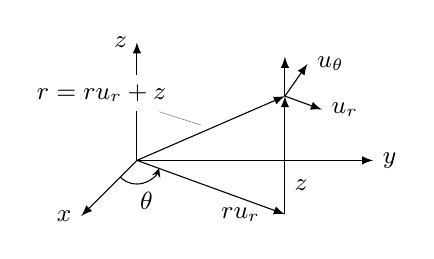
\begin{tikzpicture}[font=\small]
\pgfmathsetmacro{\len}{2}
\pgfmathsetmacro{\ang}{-20}
\draw[-latex](0,0)--++(-135:1)node[left]{$x$};
\draw[-latex](0,0)--(3,0)node[right]{$y$};
\draw[-latex](0,0)--++(0,1.5)node[left]{$z$};
\draw[-latex](0,0)--++(\ang:\len)coordinate(kB)node[pos=0.7,below]{$r\kvec{u}_r$};
\draw[-stealth]([shift={(-135:0.3)}]0,0) arc (-135:\ang:0.3)node[pos=0.6,below]{$\theta$}; 
\draw[-latex](kB)--++(0,1.5)coordinate(kT)node[pos=0.25,right]{$z\ak$};
\draw[-latex](0,0)--(kT)node[pos=0.5,pin={[fill=white,left,pin edge=-]135:{$\kvec{r}=r\kvec{u}_r+z\ak$}}]{};
\draw[-latex](kT)--++(0,0.5)node[left]{$\ak$};
\draw[-latex](kT)--++(55:0.5)node[right]{$\kvec{u}_{\theta}$};
\draw[-latex](kT)--++(\ang:0.5)node[right]{$\kvec{u}_r$};
\end{tikzpicture}
\caption{نلکی محدد میں تعین گر سمتیہ اور بنیادی  اکائی سمتیات}
\label{شکل_سمتی_تفاعل_نلکی_تعین_گر_بنیادی_اکائی}
\end{minipage}\hfill
\begin{minipage}{0.45\textwidth}
\centering
\begin{tikzpicture}
\pgfmathsetmacro{\ang}{210}
\draw[name path=oval,->-=0.8]([shift={(0:2cm and 1cm)}]0,0) arc (0:360:2cm and 1cm);
\path[name path=ray](1.25,0)--++(\ang:2.2);
\draw[-latex,name intersections={of={oval and ray}}](1.25,0)node[circ]{}node[right]{$M$}--(intersection-1)node[pos=0.25,above]{$\kvec{r}$}coordinate(kT)node[circ]{}node[above]{$m$};
\draw[opacity=0.5,very thick,-latex,gray](kT)--++(\ang:-1)node[pos=0.75,pin={[pin edge=-,fill=white,opacity=1]135:{$\kvec{F}=-\frac{GMm}{\abs{\kvec{r}}^2}\frac{\kvec{r}}{\abs{\kvec{r}}}$}}]{};
\draw[-latex](kT)--++(\ang:0.75)node[left]{$\frac{\kvec{r}}{\abs{\kvec{r}}}$};
\end{tikzpicture}
\caption{قوت کشش    دونوں کمیتوں کے بیچ سیدھے خط  پر ہو گا۔ }
\label{شکل_سمتی_تفاعل_قوت_کشش_کا_رخ}
\end{minipage}
\end{figure}
نیوٹن کے دوسرے قانون \عددی{\kvec{F}=m\ddot{\kvec{r}}}  کو مساوات \حوالہ{مساوات_سمتی_تفاعل_قوت_تجاذب_الف} کے ساتھ ملا کر
\begin{align}
m\ddot{\kvec{r}}&=-\frac{GMm}{\abs{\kvec{r}}^2}\frac{\kvec{r}}{\abs{\kvec{r}}}\nonumber\\
\ddot{\kvec{r}}&=-\frac{GM}{\abs{\kvec{r}}^2}\frac{\kvec{r}}{\abs{\kvec{r}}}\label{مساوات_سمتی_تفاعل_قوت_تجاذب_ب}
\end{align}
حاصل  ہو گا۔ سیارہ ہر لمحہ سورج کی جانب اسراع پذیر   ہے۔

مساوات \حوالہ{مساوات_سمتی_تفاعل_قوت_تجاذب_ب} کہتی ہے کہ \عددی{\kvec{r}} کا غیر سمتی مضرب \عددی{\ddot{\kvec{r}}} ہے لہٰذا 
\begin{align}\label{مساوات_سمتی_تفاعل_قوت_تجاذب_پ}
\kvec{r}\times\ddot{\kvec{r}}=\kvec{0}
\end{align}
ہو گا۔ہم دیکھتے  ہیں کہ ہ \عددی{\kvec{r}\times\ddot{\kvec{r}}}  از خود \عددی{\kvec{r}\times\dot{\kvec{r}}} کا تفرق ہے:
\begin{align}\label{مساوات_سمتی_تفاعل_قوت_تجاذب_ت}
\frac{\dif}{\dif t}(\kvec{r}\times\dot{\kvec{r}})=\underbrace{\dot{\kvec{r}}\times \dot{\kvec{r}}}_{\kvec{0}}+\kvec{r}\times\ddot{\kvec{r}}=\kvec{r}\times\ddot{\kvec{r}}
\end{align}
یوں مساوات \حوالہ{مساوات_سمتی_تفاعل_قوت_تجاذب_پ} درج ذیل کا  معادل ہے
\begin{align}\label{مساوات_سمتی_تفاعل_قوت_تجاذب_ٹ}
\frac{\dif}{\dif t}(\kvec{r}\times\dot{\kvec{r}})=\kvec{0}
\end{align}
جس کا تکمل
\begin{align}\label{مساوات_سمتی_تفاعل_قوت_تجاذب_ث}
\kvec{r}\times\dot{\kvec{r}}=\kvec{C}
\end{align}
ہے جہاں \عددی{\kvec{C}} مستقل سمتیہ ہے۔

ہمیں مساوات \حوالہ{مساوات_سمتی_تفاعل_قوت_تجاذب_ث} بتاتی ہے کہ \عددی{\kvec{r}} اور \عددی{\dot{\kvec{r}}} ہر لمحہ ایک ایسے مستوی میں ہوں گے جو \عددی{\kvec{C}} کو عمودی ہو گا۔یوں  سورج کے مرکز سے گزرتی  مستوی میں سیارے  حرکت کرتے ہیں (شکل \حوالہ{شکل_سمتی_تفاعل_سیارہ_مستوی_میں_حرکت})۔

\begin{figure}
\centering
\begin{minipage}{0.45\textwidth}
\centering
\begin{tikzpicture}
\pgfmathsetmacro{\a}{2}
\pgfmathsetmacro{\b}{1.5}
\draw(0,0)--++(\a,0)--++(45:\b)coordinate(kc)--++(-\a,0)--++(45:-\b);
\draw[-latex]($(0,0)!0.5!(kc)+(0,0.25)$)coordinate(mid)node[circ]{}node[right]{سورج}--++(0,1)node[pos=0.75,right]{$\kvec{C}=\kvec{r}\times\dot{\kvec{r}}$};
\draw([shift={(-150:1cm and 0.5cm)}]mid) arc (-150:-60:1 cm and 0.5 cm)coordinate[pos=0.25](kL);
\draw[-latex](mid)--(kL)node[pos=0.5,left]{$\kvec{r}$}node[circ]{}node[xshift=-1ex,yshift=-1ex]{سیارہ};
\draw[-latex](kL)--++(-20:0.75)node[xshift=1ex]{$\dot{\kvec{r}}$};
\end{tikzpicture}
\caption{سورج کے گرد سیارہ اس مستوی میں حرکت کرتا ہے جو \عددی{\kvec{C}=\kvec{r}\times\dot{\kvec{r}}} کو عمودی ہو اور  سورج کے کمیتی مرکز سے گزرتا ہے۔}
\label{شکل_سمتی_تفاعل_سیارہ_مستوی_میں_حرکت}
\end{minipage}\hfill
\begin{minipage}{0.45\textwidth}
\centering
\begin{tikzpicture}
\pgfmathsetmacro{\ang}{210}
\draw[name path=oval,->-=0.8]([shift={(0:2cm and 1cm)}]0,0) arc (0:360:2cm and 1cm);
\path[name path=ray](1.25,0)--++(\ang:2.2);
\draw[-latex,name intersections={of={oval and ray}}](1.25,0)node[circ]{}node[below right]{سورج}--(intersection-1)node[pos=0.5,above]{$\kvec{r}$}coordinate(kT)node[circ]{}node[below]{$P(r,\theta)$}node[above left]{سیارہ};
\draw[-latex](1.25,0)--++(1.5,0)node[below]{$\theta=0$};
\draw[-stealth]([shift={(0:0.3)}]1.25,0) arc (0:210:0.3)node[pos=0.6,shift={(135:1ex)}]{$\theta$};
\draw(2,0)node[pin=60:{\RL{حضیض شمس}}]{};
\end{tikzpicture}
\caption{حرکت سیارہ کا محددی نظام۔اوپر سے دیکھتے ہوئے حرکت، \عددی{\dot{\theta}>0} کی بنا،    گھڑی کے مخالف رخ ہے۔}
\label{شکل_سمتی_تفاعل_سیارہ_کی_حرکت}
\end{minipage}
\end{figure}
\جزوحصہء{محدد اور ابتدائی  معلومات}
ہم  نلکی محدد کے مرکز کو سورج کے  کمیتی  مرکز پر رکھتے ہیں اور سیارے کی حرکت کو  قطبی محددی سطح لیتے ہیں۔ یوں \عددی{\kvec{r}} سیارے کا تعین گر سمتیہ ہو گا  ۔یوں \عددی{\abs{\kvec{r}}=r} اور \عددی{\tfrac{\kvec{r}}{\abs{\kvec{r}}}=\kvec{u}_r} ہوں گے۔ہم  \عددی{\kvec{C}} کو محور \عددی{z} پر رکھتے ہیں لہٰذا  \عددی{\kvec{C}} کا رخ \عددی{\ak} ہو گا۔ یوں \عددی{\ak} کا \عددی{\kvec{r}\times\dot{\kvec{r}}} کے ساتھ وہی دائیں ہاتھ کا تعلق ہو گا جو اس کے ساتھ  \عددی{\kvec{C}} کا  ہے اور مثبت \عددی{z} محور سے دیکھتے ہوئے سیارہ گھڑی کے مخالف رخ گھومے   گا۔اس طرح    \عددی{t} بڑھنے سے \عددی{\theta} بڑھے گا لہٰذا تمام \عددی{t} کے لئے \عددی{ \dot{\theta}>0} ہو گا۔ہم اس لمحہ کو ابتدائی لمحہ منتخب کرتے ہیں جب سیارہ سورج کے قریب ترین ہو اور نلکی محدد کو (اگر ضرورت ہو) محور \عددی{z} کے گرد   یوں گھماتے ہیں کہ ابتدائی  لمحہ پر   \عددی{\kvec{r}}   اور  ابتدائی شعاع ہم  مکان  ہوں۔یوں ابتدائی شعاع سیارے کے  \اصطلاح{حضیض  شمس}\فرہنگ{حضیض شمس}\حاشیہب{perihelion}\فرہنگ{perihelion}  سے گزرے گا  (شکل \حوالہ{شکل_سمتی_تفاعل_سیارہ_کی_حرکت})۔

اگر ہم وقت کی پیمائش یوں کریں کہ حضیض شمسی پر \عددی{t=0} ہو تب سیارے کی حرکت کی  ابتدائی معلومات درج ذیل ہوں گی۔ 
\begin{enumerate}[a.]
\item
لمحہ \عددی{t=0} پر \عددی{r=r_0} ہو گا جو کم سے کم رداس  ہے،
\item
لمحہ \عددی{t=0} پر (\عددی{r} کی قیمت کم سے کم ہونے کی بنا)  \عددی{\dot{r}=0} ہو گا،
\item
لمحہ \عددی{t=0} پر \عددی{\theta=0} ہو گا،
\item
لمحہ \عددی{t=0} پر \عددی{\abs{\kvec{v}}=v_0} ہو گا۔\\
مزید 
\begin{align*}
v_0&=\abs{\kvec{v}}_{t=0}\\
&=\abs{\dot{r}\kvec{u}_r+r\dot{\theta}\kvec{u}_{\theta}}_{t=0}&&\text{\RL{\small{مساوات \حوالہ{مساوات_سمتی_تفاعل_قطبی_روپ_ت}}}}\\
&=\abs{r\dot{\theta}\kvec{u}_{\theta}}_{t=0}&&\text{\RL{\small{\عددی{t=0} پر \عددی{\dot{r}=0}}}}\\
&=(\abs{r\dot{\theta}}\abs{\kvec{u}_{\theta}})_{t=0}\\
&=\abs{r\dot{\theta}}_{t=0}&&\abs{\kvec{u}_{\theta}}=1\\
&=(r\dot{\theta})_{t=0}&&\text{\RL{\small{\عددی{r} اور \عددی{\dot{\theta}} دونوں مثبت ہیں}}}
\end{align*}
کی بنا ہم درج ذیل بھی جانتے ہیں۔
\item
لمحہ \عددی{t=0} پر \عددی{r\dot{\theta}=v_0} ہو گا۔
\end{enumerate}

\جزوحصہء{کپلر کا پہلا قانون  (قانون مخروط حصہ)}
کپلر کا پہلا قانون  کہتا ہے کہ  سیارے کی حرکت   مخروطی ہے جس کے ایک ماسکہ پر سورج پایا جاتا ہے۔ اس مخروط  کی سنک 
\begin{align}\label{مساوات_سمتی_تفاعل_سنک_رفتار_رداس}
e=\frac{r_0v_0^2}{GM}-1
\end{align}
اور قطبی مساوات درج ذیل ہے۔
\begin{align}\label{مساوات_سمتی_تفاعل_سنک_رداس}
r=\frac{(1+e)r_0}{1+e\cos\theta}
\end{align}

\begin{figure}
\centering
\begin{tikzpicture}
\pgfmathsetmacro{\c}{1}
\pgfmathsetmacro{\angA}{-30}
\pgfmathsetmacro{\angB}{25}
\pgfmathsetmacro{\angC}{165}
\pgfmathsetmacro{\angD}{180}
\fill[lgray](\c,0)--(\angA:2cm and 1cm) ([shift={(\angA:2cm and 1cm)}]0,0) arc (\angA:\angB:2cm and 1cm)--(\c,0);
\fill[gray](\c,0)--(\angC:2cm and 1cm) ([shift={(\angC:2cm and 1cm)}]0,0) arc (\angC:\angD:2cm and 1cm)--(\c,0);
\draw[-latex](\c,0)node[circ]{}node[below,xshift=-1ex]{سورج}--(\angB:2cm and 1cm)node[circ]{}node[right]{سیارہ}node[pos=0.5,above]{$\kvec{r}$};
\draw[name path=oval,->-=0.25]([shift={(0:2cm and 1cm)}]0,0) arc (0:360:2cm and 1cm);
\end{tikzpicture}
\caption{سورج اور سیارہ کے بیچ سیدھی لکیر مساوی اوقات میں مساوی  رقبوں کو واضح کرتی ہے۔}
\label{شکل_سمتی_تفاعل_مساوی_رقبہ_واضح}
\end{figure}
\جزوحصہء{کپلر کا دوسرا قانون (قانون یکساں رقبہ)}
کپلر کا دوسرا قانون کہتا ہے کہ سورج سے سیارہ تک رداسی سمتیہ ( جو ہمارے نمونہ میں   \عددی{\kvec{r}} ہو گا)مساوی اوقات میں مساوی   علاقوں کو واضح کرتا ہے (شکل \حوالہ{شکل_سمتی_تفاعل_مساوی_رقبہ_واضح})۔اس قانون کو اخذ کرنے کی خاطر  ہم مساوات \حوالہ{مساوات_سمتی_تفاعل_قطبی_روپ_ت} استعمال کرتے ہوئے  مساوات \حوالہ{مساوات_سمتی_تفاعل_قوت_تجاذب_ث} میں دی گئی حاصل صلیبی ضرب \عددی{\kvec{C}=\kvec{r}\times\dot{\kvec{r}}}   کی قیمت معلوم کرتے ہیں:
\begin{gather}
\begin{aligned}\label{مساوات_سمتی_تفاعل_کپلر_دوم_الف}
\kvec{C}&=\kvec{r}\times\dot{\kvec{r}}=\kvec{r}\times\kvec{v}\\
&=r\kvec{u}_r\times(\dot{r}\kvec{u}_r+r\dot{\theta}\kvec{u}_{\theta})&&\text{\RL{\small{مساوات \حوالہ{مساوات_سمتی_تفاعل_قطبی_روپ_ت}}}}\\
&=r \dot{r}\underbrace{(\kvec{u}_r\times\kvec{u}_r)}_{\kvec{0}}+r(r\dot{\theta})\underbrace{(\kvec{u}_r\times\kvec{u}_{\theta})}_{\ak}\\
&=r(r\dot{\theta})\ak
\end{aligned}
\end{gather}
لمحہ \عددی{t=0} پر اس سے درج ذیل حاصل ہو گا۔
\begin{align}\label{مساوات_سمتی_تفاعل_کپلر_دوم_ب}
\kvec{C}=[r(r\dot{\theta})]_{t=0}\ak=r_0v_0\ak
\end{align}
مساوات \حوالہ{مساوات_سمتی_تفاعل_کپلر_دوم_الف} میں \عددی{\kvec{C}} کی یہ   قیمت  پر کرنے سے درج ذیل حاصل ہو گا۔
\begin{align}\label{مساوات_سمتی_تفاعل_کپلر_دوم_پ}
r^2\dot{\theta}=r_0v_0\quad \text{یعنی}\quad r_0v_0\ak=r^2\dot{\theta}\ak
\end{align}
قطبی محدد میں  تفرقی رقبہ درج ذیل لکھا جاتا ہے (حصہ \حوالہ{حصہ_مخروط_قطبی_محدد_میں_تکمل})۔
\begin{align*}
\dif S=\frac{1}{2}r^2\dif \theta
\end{align*}
یوں \عددی{\tfrac{\dif S}{\dif t}} کی   قیمت ایک مستقل ہے:
\begin{align}\label{مساوات_سمتی_تفاعل_کپلر_دوم_ت}
\frac{\dif S}{\dif t}=\frac{1}{2}r^2\dot{\theta}=\frac{1}{2}r_0v_0
\end{align} 
جو کپلر کا دوسرا قانون  ہے۔

زمین کے لئے   \عددی{r_0} تقریباً    \عددی{\SI{1.5e8}{\kilo\meter}}، \عددی{v_0} تقریباً \عددی{\SI{30}{\kilo\meter\per\second}}  ہے لہٰذا \عددی{\tfrac{\dif S}{\dif t}}تقریباً \عددی{\SI{2.25e9}{\kilo\meter\squared\per\second}} ہو گا۔یوں آپ کے دل کی ہر ایک  دھڑکن میں  زمین اپنے مدار میں  \عددی{\SI{30}{\kilo\meter}} فاصلہ طے کرتی ہے اور سورج سے زمین تک رداسی خط \عددی{\SI{2.25e9}{\kilo\meter\squared}} رقبہ واضح کرتا ہے۔ 

\جزوحصہء{کپلر کے پہلے قانون کا ثبوت}
یہ دکھانے کی خاطر کہ سورج کے گرد سیارے  کا  مدار مخروطی ہوتا ہے   جس کے ایک ماسکہ پر سورج واقع ہوتا ہے، ہمیں \عددی{r} کو متغیر \عددی{\theta} کا تفاعل لکھنا ہو گا۔ایسا کرنے کی خاطر ہمیں ایک لمبا حساب کرنا ہو گا۔ 

ہم وقتی طور پر \عددی{\dot{\theta}} سے چھٹکارا حاصل کرنے کی خاطر   مساوات \حوالہ{مساوات_سمتی_تفاعل_قطبی_روپ_ث} اور مساوات \حوالہ{مساوات_سمتی_تفاعل_قوت_تجاذب_ب} میں \عددی{\kvec{u}_r=\tfrac{\kvec{r}}{\abs{\kvec{r}}}} کے عددی سر ایک دوسرے کے برابر پر لکھ کر درج ذیل مساوات حاصل کرتے ہیں۔
\begin{align}\label{مساوات_سمتی_تفاعل_کپلر_ثبوت_پہلا_الف}
\ddot{r}-r\dot{\theta}^2=-\frac{GM}{r^2}
\end{align}
اس میں ہم  مساوات \حوالہ{مساوات_سمتی_تفاعل_کپلر_دوم_پ} سے  \عددی{\dot{\theta}} کی جگہ   \عددی{\tfrac{r_0v_0}{r^2}} پر کر کے ترتیب دیتے  ہوئے
\begin{align}\label{مساوات_سمتی_تفاعل_کپلر_ثبوت_پہلا_ب}
\ddot{r}=\frac{r_0^2v_0^2}{r^3}-\frac{GM}{r^2}
\end{align}
حاصل کرتے ہیں۔ہم متغیرات تبدیل کرتے ہوئے اس سے درجہ اول کی تفرقی مساوات حاصل کرتے ہیں۔یوں زنجیری قاعدہ  استعمال کرتے ہوئے
\begin{align*}
p=\frac{\dif r}{\dif t},\quad \frac{\dif^2r}{\dif t^2}=\frac{\dif p}{\dif t}=\frac{\dif p}{\dif r}\frac{\dif r}{\dif t}=p\frac{\dif p}{\dif r}
\end{align*}
لکھ کر مساوات  \حوالہ{مساوات_سمتی_تفاعل_کپلر_ثبوت_پہلا_ب} درج  ذیل صورت اختیار کرتی ہے۔
\begin{align}\label{مساوات_سمتی_تفاعل_کپلر_ثبوت_پہلا_پ}
p\frac{\dif p}{\dif r}=\frac{r_0^2v_0^2}{r^3}-\frac{GM}{r^2}
\end{align}
دونوں اطراف کو \عددی{2} سے ضرب کرتے ہوئے \عددی{r} کے لحاض سے تکمل لیتے ہیں۔
\begin{align}\label{مساوات_سمتی_تفاعل_کپلر_ثبوت_پہلا_ت}
p^2=(\dot{r})^2=-\frac{r_0^2v_0^2}{r^2}+\frac{2GM}{r}+C_1
\end{align}
لمحہ \عددی{t=0} پر ابتدائی معلومات \عددی{r=r_0} اور \عددی{\dot{r}=0}  سے \عددی{C_1} کی قیمت تعین ہو گی۔
\begin{align*}
C_1=v_0^2-\frac{2GM}{r_0}
\end{align*}
اس طرح مساوات \حوالہ{مساوات_سمتی_تفاعل_کپلر_ثبوت_پہلا_ت}  کو ترتیب دینے کے بعد درج ذیل لکھا جا سکتا ہے۔
\begin{align}\label{مساوات_سمتی_تفاعل_کپلر_ثبوت_پہلا_ٹ}
\dot{r}^2=v_0^2\big(1-\frac{r_0^2}{r^2}\big)+2GM\big(\frac{1}{r}-\frac{1}{r_0}\big)
\end{align}

مساوات  \حوالہ{مساوات_سمتی_تفاعل_کپلر_ثبوت_پہلا_الف} سے مساوات \حوالہ{مساوات_سمتی_تفاعل_کپلر_ثبوت_پہلا_ٹ}  حاصل کرنے میں ہم نے  \عددی{r} کی دو درجی  تفرقی مساوات سے \عددی{r}  کی ایک درجی تفرقی مساوات حاصل کی۔ ہمیں اب \عددی{\theta} کی روپ میں \عددی{r} کو  لکھنا باقی ہے   لہٰذا ہم \عددی{\theta} کو دوبارہ مساوات میں لاتے ہیں۔ایسا کرنے کی خاطر  مساوات \حوالہ{مساوات_سمتی_تفاعل_کپلر_ثبوت_پہلا_ٹ}  کے دونوں اطراف کو مساوات \عددی{r^2\dot{\theta}=r_0v_0} (مساوات \حوالہ{مساوات_سمتی_تفاعل_کپلر_دوم_پ}) کے مطابقتی اطراف سے تقسیم کر  کے حقیقت
 \عددی{\tfrac{\dot{r}}{\dot{\theta}}=\tfrac{\dif r/\dif t}{\dif\theta/\dif t}=\tfrac{\dif r}{\dif\theta}} بروئے کار لاتے ہوئے درج ذیل حاصل کرتے ہیں۔
\begin{align}\label{مساوات_سمتی_تفاعل_کپلر_ثبوت_پہلا_ث}
\frac{1}{r^4}\big(\frac{\dif r}{\dif\theta}\big)^2&=\frac{1}{r_0^2}-\frac{1}{r^2}+\frac{2GM}{r_0^2v_0^2}\big(\frac{1}{r}-\frac{1}{r_0}\big)\\
&=\frac{1}{r_0^2}-\frac{1}{r^2}+2h\big(\frac{1}{r}-\frac{1}{r_0}\big)&&h=\frac{GM}{r_0^2v_0^2}
\end{align}
اس کی مزید سادہ صورت حاصل کرنے کی خاطر  ہم درج ذیل پر کرتے ہیں۔
 \begin{align*}
u=\frac{1}{r},\quad u_0=\frac{1}{r_0},\quad \frac{\dif u}{\dif\theta}=-\frac{1}{r^2}\frac{\dif r}{\dif \theta},\quad \big(\frac{\dif u}{\dif\theta}\big)^2=\frac{1}{r^4}\big(\frac{\dif r}{\dif\theta}\big)^2
\end{align*}
یوں  درج ذیل حاصل ہو گا۔
\begin{align}
\big(\frac{\dif u}{\dif\theta}\big)^2&=u_0^2-u^2+2hu-2hu_0=(u_0-h)^2-(u-h)^2\label{مساوات_سمتی_تفاعل_کپلر_ثبوت_پہلا_ج}\\
\frac{\dif u}{\dif \theta}&=\mp\sqrt{(u_0-h)^2-(u-h)^2}\label{مساوات_سمتی_تفاعل_کپلر_ثبوت_پہلا_چ}
\end{align}

ہمیں کس علامت کا انتخاب کرنا ہو گا؟ ہم جانتے ہیں کہ \عددی{\dot{\theta}=\tfrac{r_0v_0}{r^2}} مثبت ہے۔ساتھ ہی \عددی{t=0} پر \عددی{r} کم سے کم قیمت سے شروع ہوتا ہے لہٰذا یہ یکدم گھٹ نہیں سکتا ہے، اور ابتدائی مثبت  لمحات میں \عددی{\dot{r}\ge 0}   ہو گا لہٰذا
\begin{align*}
\frac{\dif u}{\dif\theta}=-\frac{1}{r^2}\frac{\dif r}{\dif\theta}\le 0\quad\text{اور}\quad\frac{\dif r}{\dif\theta}=\frac{\dot{r}}{\dot{\theta}}\ge 0
\end{align*}
ہو گا۔مساوات \حوالہ{مساوات_سمتی_تفاعل_کپلر_ثبوت_پہلا_چ} میں منفی علامت درست ہو گی۔ یہ جاننے کے بعد ہم مساوات \حوالہ{مساوات_سمتی_تفاعل_کپلر_ثبوت_پہلا_چ} کو ترتیب دے کر  \عددی{\theta} کے لحاض سے دونوں اطراف اک تکمل لیتے ہیں۔
\begin{gather}
\begin{aligned}\label{مساوات_سمتی_تفاعل_کپلر_ثبوت_پہلا_ح}
\frac{-1}{\sqrt{(u_0-h)^2-(u-h)^2}}\frac{\dif u}{\dif\theta}&=1\\
\cos^{-1}\big(\frac{u-h}{u_0-h}\big)&=\theta+C_2
\end{aligned}
\end{gather}
چونکہ \عددی{\theta=0} پر \عددی{u=u_0}  ہو گا اور \عددی{\cos^{-1}(1)=0} ہوتا ہے لہٰذا \عددی{C_2} صفر ہو گا۔یوں
\begin{align}\label{مساوات_سمتی_تفاعل_کپلر_ثبوت_پہلا_خ}
\frac{u-h}{u_0-h}=\cos\theta
\end{align}
اور
\begin{align}\label{مساوات_سمتی_تفاعل_کپلر_ثبوت_پہلا_د}
\frac{1}{r}=u=h+(u_0-h)\cos\theta
\end{align}
ہو گا جس کو چند الجبرائی اقدام کے بعد
\begin{align}\label{مساوات_سمتی_تفاعل_کپلر_ثبوت_پہلا_ڈ}
r=\frac{(1+e)r_0}{1+e\cos\theta}
\end{align}
لکھا جا سکتا ہے جہاں 
\begin{align}\label{مساوات_سمتی_تفاعل_کپلر_ثبوت_پہلا_ذ}
e=\frac{1}{r_0h}-1=\frac{r_0v_0^2}{GM}-1
\end{align}
ہوں گے۔ مساوات \حوالہ{مساوات_سمتی_تفاعل_کپلر_ثبوت_پہلا_ڈ} اور مساوات \حوالہ{مساوات_سمتی_تفاعل_کپلر_ثبوت_پہلا_ذ} مل کر  کہتے ہیں کہ سیارے کی راہ مخروطی ہو گی جس کے ایک ماسکہ پر سورج ہو گا اور جس کی سنک \عددی{e=\tfrac{r_0v_0^2}{GM}-1} ہو گی۔ یہ قانون کپلر اول    کی جدید مساوات ہے۔


\جزوحصہء{کپلر کا تیسرا قانون (قانون وقت اور فاصلہ)}
ایک سیارہ جتنے وقت \عددی{T} میں اپنے سورج کے گرد ایک چکر کاٹتا  ہے، اس کو سیارہ کا \اصطلاح{دوری عرصہ }\فرہنگ{دوری عرصہ}\حاشیہب{orbital period}\فرہنگ{orbital period}کہتے ہیں۔ کپلر کا تیسرا قانون کہتا ہے کہ \عددی{T} اور سیارے کے مدار  کے نصف محور اکبر \عددی{a} کے بیچ درج ذیل تعلق پایا جاتا ہے۔
\begin{align}\label{مساوات_سمتی_تفاعل_کپلر_تیسرا_الف}
\frac{T^2}{a^3}=\frac{4\pi^2}{GM}
\end{align} 
چونکہ کسی بھی شمسی نظام کے اندر  اس مساوات کا   دایاں ہاتھ ایک مستقل ہو گا   لہٰذا اس نظام میں تمام سیاروں کے لئے \عددی{T^2} اور \عددی{a^3} کا تناسب یکساں ہو گا۔ 

کپلر کا تیسرا قانون  ہمیں ہمارے نظام شمسی  کی جسامت کی معلومات حاصل کرنے کا موقع دیتا ہے۔   ہم ہر ایک سیارے کے نصف محور اکبر کو فلکیاتی اکائیوں میں لکھ سکتے ہیں۔زمین کے   نصف محور اکبر کی لمبائی     فلکیاتی اکائی کہلاتی ہے۔ہم  کسی بھی لمحہ تمام سیاروں کے بیچ فاصلوں کو بھی فلکیاتی اکائیوں میں لکھ سکتے ہیں۔ اب آخری کام،   ان تمام فاصلوں میں کسی ایک کی لمبائی، کلومیٹروں میں  معلوم کرنا رہ گیا ہے۔زھرہ  سے  ٹکرا نے کے بعد ریڈار کی   واپس پلٹی  موجوں سے ہم زمین اور زھرہ کے بیچ فاصلہ ناپ سکتے ہیں۔ اس قسم کے تجربات سے ہم اب جانتے ہیں کہ ایک فلکیاتی اکائی \عددی{\SI{149597870}{\kilo\meter}} کے برابر ہے۔ 

ہم سیارے کے ترخیمی مدار  میں گھیرے گئے رقبہ کے دو مختلف  کلیات کو ملا کر  کپلر کا تیسرا قانون اخذ کرتے ہیں:
\begin{align*}
\text{رقبہ}&=\pi ab&&\text{\RL{کلیہ 1}}\\
\text{رقبہ}&=\int_0^T\dif S&&\text{\RL{کلیہ 2}}\\
&=\int_0^T\frac{1}{2}r_0v_0\dif t&&\text{\RL{مساوات \حوالہ{مساوات_سمتی_تفاعل_کپلر_دوم_ت}}}\\
&=\frac{1}{2}Tr_0v_0
\end{align*} 
ان دو مساوات کو ایک دوسرے کے مساوی رکھتے ہوئے  درج ذیل حاصل ہو گا۔
\begin{align}\label{مساوات_سمتی_تفاعل_کپلر_تیسرا_ب}
T&=\frac{2\pi ab}{r_0v_0}=\frac{2\pi a^2}{r_0v_0}\sqrt{1-e^2}&& \text{\RL{ترخیم کے لئے \عددی{b=a\sqrt{1-e^2}} ہوتا ہے}}
\end{align}

ہمیں اب \عددی{a} اور \عددی{e} کو \عددی{r_0}، \عددی{v_0}، \عددی{G} اور \عددی{M} کی روپ میں لکھنا ہے۔ مساوات \حوالہ{مساوات_سمتی_تفاعل_کپلر_ثبوت_پہلا_ذ} ہمیں \عددی{e} دیتی ہے جبکہ مساوات  \حوالہ{مساوات_سمتی_تفاعل_کپلر_ثبوت_پہلا_ڈ} میں  \عددی{\theta} کو \عددی{\pi} کے برابر پر کرنے سے 
\begin{align*}
r_{\text{بلندتر}}&=r_0\frac{1+e}{1-e}
\end{align*}
حاصل ہوتا ہے لہٰذا \عددی{a} کے لئے درج ذیل ہو گا۔
\begin{align}\label{مساوات_سمتی_تفاعل_کپلر_تیسرا_پ}
2a=r_0+r_{\text{بلندتر}}=\frac{2r_0}{1-e}=\frac{2r_0GM}{2GM-r_0v_0^2}
\end{align}
مساوات \حوالہ{مساوات_سمتی_تفاعل_کپلر_تیسرا_ب} کے دونوں اطراف کا مربع  لے کر اس میں مساوات \حوالہ{مساوات_سمتی_تفاعل_کپلر_ثبوت_پہلا_ذ} اور مساوات \حوالہ{مساوات_سمتی_تفاعل_کپلر_تیسرا_پ} کے نتائج پر کرنے سے کپلر کا تیسرا قانون حاصل ہو گا (سوال \حوالہ{سوال_سمتی_تفاعل_اشتقاق_کپلر_تیسرا})۔


\جزوحصہء{مدار}
اگرچہ کپلر نے یہ قوانین تجرباتی طور پر  دریافت کیے، قوانین نیوٹن سے قوانین کپلر  کے حصول کے بعد ہم جانتے ہیں کہ یہ قوانین ہر اس جسم پر لاگو ہوں گے جس  پر  بالعکس مربع  قانون کے تحت  قوت لاگو ہو۔یہ سورج کے گرد  ہالی دم دار ستارہ اور   آئکارس سیارچہ کی  مدار   اور زمین کے گرد چاند  کے مدار پر لاگو ہوں گے۔اسی طرح یہ چاند کے گرد اپالو 8 کے خلائی جہاز  کے مدار پر بھی لاگو ہوتے ہیں۔ایٹم کے مرکزہ   پر مارے گئے  بار بردار ذرات قوانین کپلر  کو مطمئن کرتے ہوئے قطع زائد راہوں پر فشاں ہوتے ہیں۔

جدول \حوالہ{جدول_سمتی_تفاعل_شمسی_سیارے} میں نظام شمسی کے    سیاروں کے مدار کی معلومات دی گئی ہے۔مصنوعی سیاروں کے حاصل مواد سے ہم  سمندروں میں پانی کی سطح میں فرق جان سکے اور  بحر الکاہل میں  دور ترین جزیروں  کا درست مقام معلوم کر سکے۔اس مواد سے ہمیں یہ بھی معلوم ہوا کہ سورج اور چاند کی قوت کشش  زمین کے گرد مصنوعی سیاروں کے مدار پر  اثر انداز ہوں گے اور شمسی  اخراج اتنا دباو پیدا کرتا ہے کہ مدار    کی شکل تبدیل ہو جائے۔

جدول \حوالہ{جدول_سمتی_تفاعل_مصنوعی_سیارے_مواد} اور جدول \حوالہ{جدول_سمتی_تفاعل_اعدادی_مواد}  میں مزید مواد  پیش کیا گیا ہے۔

\begin{table}
\caption{شمسی سیاروں کے \عددی{a}، \عددی{e} اور \عددی{T} کی قیمتیں۔}
\label{جدول_سمتی_تفاعل_شمسی_سیارے}
\centering
\begin{tabular}{
lrrr
}
\toprule
سیارہ&نصف  محور  \عددی{a^{\dagger}} & سنک \عددی{e} & دوری عرصہ \عددی{T}\\
\midrule
عطارہ&57.95&0.2056&87.967 دن \\
زھرہ&108.11&0.0068&224.701 دن\\
زمین&149.57&0.0167&365.256 دن\\
مریخ&227.84&0.0934&1.8808 سال\\
مشتری&778.14&0.0484&11.8613 سال\\
زحل&1427.0&0.0543&29.4568 سال\\
یورانس&2870.3&0.0460&84.0081 سال\\
نیپچون&4499.9&0.0082&164.784 سال\\
پلوٹو&5909&0.2481&248.35 سال\\
\multicolumn{3}{l}{
\عددی{^{\dagger}} ملین  کلومیٹر (\عددی{\SI{e6}{\kilo\meter}})}\\
\bottomrule
\end{tabular}
\end{table}
%=====================
\begin{table}
\caption{زمین کے گرد مصنوعی سیاروں  کی معلومات}
\label{جدول_سمتی_تفاعل_مصنوعی_سیارے_مواد}
\centering
\begin{tabular}{rrrrrrrrr}
\toprule
نام&پرواز&خلائی زندگی&کمیت&
\begin{minipage}{0.75cm}
دوری\\
عرصہ\عددیء{^{\dagger\dagger}}
\end{minipage}
&حضیض \عددیء{^\dagger}&اوج  \عددیء{^\dagger}&
\begin{minipage}{1cm}
نصف محور\\
اکبر \عددیء{^{\dagger}}
\end{minipage}
&سنک\\
\midrule
سپٹنک 1&اکتوبر 1957&57.6 دن&83.6&96.2&215&939&6955&0.052\\
ونگارڈ  1&مارچ 1958&300 سال&1.47&138.5&649&4340&8872&0.208\\
سنکام 3&اگست 1964&\عددی{>10^6} سال&39&1436.2&35718&35903&42189&0.002\\
سکائے لیب 4&نومبر 1973&84.06 دن&13980&93.11&422&437&6808&0.001\\
ٹائرس 11&اکتوبر 1978&500 سال&734&102.12&850&866&7236&0.001\\
گوس 4&ستمبر 1980&\عددی{>10^6} سال&627&1436.2&35776&35800&42166&0.0003\\
انٹل سیٹ 5&دسمبر 1980&\عددی{>10^6} سال&1928&1417.67&35143&35707&41803&0.007\\
\multicolumn{3}{r}{\عددی{^{\dagger}} کلو میٹر}\\
\multicolumn{3}{r}{\عددی{^{\dagger\dagger}} منٹ}\\
\bottomrule
\end{tabular}
\end{table}
%=========================
\begin{table}
\caption{اعدادی مواد}
\label{جدول_سمتی_تفاعل_اعدادی_مواد}
\centering
\begin{tabular}{rr}
\toprule
تجاذبی مستقل & \عددی{\SI{6.6720e-11}{\newton\meter\squared\per\kilo\gram\squared}}\\
کمیت شمس&\عددی{\SI{1.99e30}{\kilo\gram}}\\
کمیت زمین&\عددی{\SI{5.975e24}{\kilo\gram}}\\
استوائی رداس  زمین&\عددی{\SI{6378.533}{\kilo\meter}}\\
قطبی رداس زمین&\عددی{\SI{6356.912}{\kilo\meter}}\\
زمین  کا ہم  دوری عرصہ&\عددی{1436.1} منٹ\\
زمین کا سورج کے گرد دوری عرصہ&\عددی{365.256} دن (ایک سال)\\
\bottomrule
\end{tabular}
\end{table}
%=======================

\جزوحصہء{سوالات}
\ابتدا{سوالات}
\ابتدا{سوال}
سکائے  لیب  4 کا نصف محور اکبر \عددی{a=\SI{6808}{\kilo\meter}} ہے۔کپلر کے تیسرے قانون  میں زمین کی کمیت کو \عددی{M} لیتے ہوئے دوری عرصہ  معلوم کیا جا سکتا ہے۔اس کا حساب لگائیں۔ جدول \حوالہ{جدول_سمتی_تفاعل_مصنوعی_سیارے_مواد} میں دی گئی  قیمت کے ساتھ موازنہ کریں۔
\انتہا{سوال}  
%=========
\ابتدا{جواب}
\wf{\unexpanded{
$T=\SI{93.2}{\minute}$
}}
\انتہا{جواب}
%===============
\ابتدا{سوال}
حضیض شمسی پر سورج سے زمین کا فاصلہ تقریباً \عددی{\SI{149577000}{\kilo\meter}} ہو تا ہے اور  سورج کے گرد زمین کے مدار کی سنک \عددی{0.0167} ہے۔ حضیض شمس پر زمین کی رفتار \عددی{v_0} تلاش کریں (مساوات \حوالہ{مساوات_سمتی_تفاعل_سنک_رفتار_رداس} استعمال کریں)۔
\انتہا{سوال}
%==============
\ابتدا{سوال}
روس نے جولائی \سن{1965} میں پروٹان  1، مصنوعی سیارہ مدار میں چھوڑا جس کی کمیت  (چھوڑتے وقت ) \عددی{\SI{12200}{\kilo\gram}}،  بلندی حضیض \عددی{\SI{183}{\kilo\meter}}، بلندی اوج \عددی{\SI{589}{\kilo\meter}} اور دوری عرصہ \عددی{92.25} منٹ  تھا۔  زمین کی کمیت اور تجاذبی مستقل  کی قیمتیں استعمال کر کے مساوات \حوالہ{مساوات_سمتی_تفاعل_کپلر_تیسرا_الف} سے  نصف محور اکبر \عددی{a}  تلاش کریں۔اس کا موازنہ اس عدد سے کریں جو حضیض اور اوج کے مجموعہ کے ساتھ  زمین کا قطر جمع  کرنے سے حاصل ہو گا۔
\انتہا{سوال}  
%=========
\ابتدا{جواب}
\wf{\unexpanded{
$a=\SI{6763}{\kilo\meter}$
}}
\انتہا{جواب}
%==============
\ابتدا{سوال}
(ا)  وائکنگ 1 مصنوعی سیارہ ، جس کا دوری عرصہ \عددی{1639} منٹ تھا ، نے   اگست 1975 تا جون 1976 مریخ کا جائزہ  کیا۔  مریخ کی کمیت \عددی{\SI{6.418e23}{\kilo\gram}} لیتے ہوئے  وائکنگ 1 کا نصف محور اکبر تلاش کریں۔ (ب) مریخ کی سطح  سے وائکنگ 1 کا کم سے کم فاصلہ \عددی{\SI{1499}{\kilo\meter}} اور زیادہ سے زیادہ فاصلہ \عددی{\SI{35800}{\kilo\meter}}  تھا۔ ان حقائق اور جزو-ا میں حاصل نتائج کو  استعمال کرتے ہوئے مریخ کے اوسط  قطر کی   اندازاً  قیمت معلوم کریں۔
\انتہا{سوال}
%============
\ابتدا{سوال}
وائکنگ 2  مصنوعی سیارہ نے ستمبر 1975 تا اگست 1976  مریخ کا جائزہ  کیا۔ اس کے نصف محور اکبر \عددی{\SI{22030}{\kilo\meter}} تھا۔ اس کا دوری عرصہ دریافت کریں۔
\انتہا{سوال}  
%=========
\ابتدا{جواب}
\wf{\unexpanded{
$T=\SI{1655}{\minute}$
}}
\انتہا{جواب}
%==============
\ابتدا{سوال}\ترچھا{ہم عصر  مدار}\\
زمین کی استوائی مستوی میں کئی مصنوعی سیاروں  کے مدار تقریباً دائری ہے اور ان کا دوری عرصہ عین  ایک دن کے برابر ہے۔  یوں یہ بلندی پر رہتے ہوئے   سطح زمین کے اوپر ساکن نظر آتے ہیں۔ ایسے مدار کو \اصطلاح{ہم عصر مدار}\فرہنگ{مدار!ہم عصر}\حاشیہب{geosynchronous orbit, geostationary orbit}\فرہنگ{orbit!geosynchronous}\فرہنگ{orbit!geostationary} کہتے ہیں۔
\begin{enumerate}[a.]
\item
ہم عصر مصنوعی سیارے کا نصف محور اکبر تقریباً کتنا ہو گا؟ اپنے جواب کی وجہ پیش کریں۔
\item
زمین کی سطح سے ہم عصر مدار کتنی  بلندی پر ہو گا؟
\item
جدول  \حوالہ{جدول_سمتی_تفاعل_مصنوعی_سیارے_مواد} میں دیے گئے مصنوعی سیاروں میں کس کا مدار تقریباً ہم عصر ہے؟
\end{enumerate}
\انتہا{سوال}
%===================
\ابتدا{سوال}
مریخ کی کمیت \عددی{\SI{6.418e23}{\kilo\gram}} ہے  جبکہ مریخ کا ایک  دن \عددی{1477.4} منٹ  ہے۔مریخ کے گرد مدار میں ایک مصنوعی سیارہ جس کا  دوری عرصہ مریخی دن کے برابر ہو، سطح مریخ سے کتنی بلندی پر ہو گا؟ اپنے جواب کی وجہ پیش کریں۔
\انتہا{سوال}  
%=========
\ابتدا{جواب}
\wf{\unexpanded{
$a=\SI{20430}{\kilo\meter}$
}}
\انتہا{جواب}
%===========
\ابتدا{سوال}
زمین کے گرد چاند  کا دوری عرصہ \عددی{\num{2.36055e6}} سیکنڈ  ہے۔چاند کتنا دور ہے؟
\انتہا{سوال}
%==============
\ابتدا{سوال}
زمین کے گرد ایک مصنوعی سیارہ دائری مدار میں حرکت کرتا  ہے۔ مصنوعی سیارے کی رفتار کو مدار کے رداس کا تفاعل لکھیں۔
\انتہا{سوال}  
%=========
\ابتدا{جواب}
\wf{\unexpanded{
$\abs{v}=1.9966\times 10^7r^{-1/2}\,\si{\meter\per\second}$
}}
\انتہا{جواب}
%==============
\ابتدا{سوال}
نظام شمسی میں سیاروں کا \عددی{\tfrac{T^2}{a^3}} کتنا ہو گا؟ زمین کے گرد مصنوعی سیاروں کے لئے کتنا ہو گا؟ چاند کے گرد مصنوعی سیاروں کے لئے یہ کتنا ہو گا؟ (چاند کی کمیت \عددی{\SI{7.354e22}{\kilo\gram}} ہے۔)
\انتہا{سوال}
%==============
\موٹا{بغیر کیلکولیٹر استعمال کئے قلم و کاغذ سے حل کریں}\\
\ابتدا{سوال}
مساوات \حوالہ{مساوات_سمتی_تفاعل_سنک_رفتار_رداس} میں  \عددی{v_0} کی کس قیمت کے لئے  مساوات \حوالہ{مساوات_سمتی_تفاعل_سنک_رداس} کا مدار دائری ہو گا؟ ترخیمی ہو گا؟ قطع مکافی ہو گا؟ قطع زائد ہو گا؟
\انتہا{سوال}  
%=========
\ابتدا{جواب}
\wf{\unexpanded{
دائرہ: \عددی{v_0=\sqrt{\tfrac{GM}{r_0}}}؛ ترخیم: \عددی{\sqrt{\tfrac{GM}{r_0}}<v_0<\sqrt{\tfrac{2GM}{r_0}}}؛ قطع مکافی : \عددی{v_0=\sqrt{\tfrac{2GM}{r_0}}}؛ قطع زائد: \عددی{v_0>\sqrt{\tfrac{2GM}{r_0}}}
}}
\انتہا{جواب}
%==========
\ابتدا{سوال}
دکھائیں کہ دائری مدار میں سیارہ یکساں رفتار سے حرکت کرتا ہے۔ (اشارہ: یہ قوانین کپلر کی بدولت ہو گا۔)
\انتہا{سوال}
%================
\ابتدا{سوال}
فرض کریں  ایک مستوی میں متحرک ذرے کا تعین گر سمتیہ \عددی{\kvec{r}} ہے اور  یہ  سمتیہ \عددی{\tfrac{\dif S}{\dif t}} کی شرح سے رقبہ واضح کرتا ہے۔محدد متعارف کئے بغیر اور مطلوبہ تفرقات  کی موجودگی تصور کرتے ہوئے، بڑھوتری اور حد  پر مبنی  درج ذیل مساوات کی  جیومیٹریائی جواز پیش کریں۔ 
\begin{align*}
\frac{\dif S}{\dif t}=\frac{1}{2}\abs{\kvec{r}\times \dot{\kvec{r}}}
\end{align*}
\انتہا{سوال}
%============
\ابتدا{سوال}\شناخت{سوال_سمتی_تفاعل_اشتقاق_کپلر_تیسرا}
کپلر کے تیسرے قانون  کا اشتقاق  پورا کریں (مساوات \حوالہ{مساوات_سمتی_تفاعل_کپلر_تیسرا_ب} کے بعد  حصہ۔)
\انتہا{سوال}
%============
\ابتدا{سوال}
کسی ستارہ کے گرد دو سیارے دائری مدار میں  طواف  کرتے ہیں۔سیارہ \عددی{A} ستارے کے  قریب ہے جبکہ سیارہ \عددی{B}ستارہ سے  زیادہ فاصلہ پر ہے۔فرض کریں لمحہ \عددی{t} پر ان کے مقام  بالترتیب 
\begin{align*}
\kvec{r}_A(t)&=2\cos(2\pi t)\ai+2\sin(2\pi t)\aj\\
\kvec{r}_B(t)&=3\cos(\pi t)\ai+3\sin(\pi t)\aj
\end{align*}
ہیں جہاں ستارہ کا مقام مبدا ہے اور فاصلوں کو فلکیاتی اکائیوں میں ناپا گیا ہے۔ (دھیان رہے کہ سیارہ \عددی{A} کی رفتار سیارہ \عددی{B} سے زیادہ ہے۔)

سیارہ \عددی{A} پر رہائش پذیر  لوگوں کا خیال ہے کہ ان کا سیارہ، ان کے شمسی نظام کا مرکز ہے۔
\begin{enumerate}[a.]
\item
سیارہ \عددی{A} کو نئی محددی نظام کا  مبدا  تصور کرتے ہوئے سیارہ \عددی{B} کے مقام کی مقدار معلوم مساوات تلاش کریں۔ اپنا جواب \عددی{\cos(\pi t)} اور \عددی{\sin(\pi t)}کی صورت میں لکھیں۔
\item
سیارہ \عددی{A} کو مبدا  تصور کرتے ہوئے  سیارہ \عددی{B} کی راہ ترسیم کریں۔

آپ دیکھ سکتے ہیں کہ ان لوگوں کو سیاروں کی حرکت سمجھنے میں کتنی دشواری ہو گی۔ کپلر سے پہلے یہی حال ہمارا تھا۔ 
\end{enumerate}
\انتہا{سوال}  
%=========
\ابتدا{جواب}
\wf{\unexpanded{
(ا)  \عددی{x(t)=2+(3-4\cos (\pi t))\cos (\pi t)}\\
\عددی{y(t)=(3-4\cos(\pi t))\sin(\pi t)}
}}
\انتہا{جواب}
%================
\ابتدا{سوال}
کپلر نے دریافت کیا  کہ سورج کے گرد زمین ترخیمی راہ  پر  طواف کرتی ہے اور سورج اس کے ایک ماسکہ پر پایا جاتا ہے۔ سورج کے مرکز سے زمین کے مرکز تک لمحہ \عددی{t} پر تعین گر  سمتیہ \عددی{\kvec{r}(t)} لیں۔ زمین کے جنوبی قطب  سے شمالی قطب تک سمتیہ \عددی{\kvec{w}} لیں۔ہم جانتے ہیں کہ \عددی{\kvec{w}} مستقل ہے اور ترخیم  کے مستوی  کو عمودی نہیں ہے (زمین کا محور  جھکا  ہے)۔ سمتیات \عددی{\kvec{w}} اور \عددی{\kvec{r}(t)} کے روپ میں (ا)  حضیض شمسی، (ب) اوج شمسی، (ج)  اعتدالین  (جب دن اور رات ایک دوسرے کے برابر ہوں)، (د) لمبا ترین دن (گرم ترین دن)، (ہ) چھوٹا ترین دن ( سرد ترین دن) کے  ریاضی  معنی  پیش کریں۔
\انتہا{سوال}
%========
\موٹا{نلکی محددی نظام}\\
\ابتدا{سوال}\ترچھا{نلکی محدد میں مقام اور حرکت کے اکائی سمتیات ۔}\\
فضا میں متحرک ذرے  کا مقام نلکی محدد میں لکھتے ہوئے ہم 
\begin{align*}
\kvec{u}_r=\cos(\theta)\ai+(\sin\theta)\aj,\,\kvec{u}_{\theta}=-(\sin\theta)\ai+(\cos\theta)\aj
\end{align*}
اور \عددی{\ak} اکائی سمتیات استعمال کرتے ہیں۔یوں  متحرک ذرے کا  تعین گر سمتیہ  \عددی{\kvec{r}=r\kvec{u}_r+z\ak} ہو گا جہاں \عددی{r} مبدا سے  ذرے کا مثبت قطبی فاصلہ ہے۔
\begin{enumerate}[a.]
\item
دکھائیں کہ \عددی{\kvec{u}_r}، \عددی{\kvec{u}_{\theta}} اور \عددی{\ak}، اسی ترتیب میں، اکائی سمتیات کا دایاں ہاتھ چھوکٹ  دیتے ہیں۔
\item
درج ذیل دکھائیں۔
\begin{align*}
\frac{\dif\kvec{u}_r}{\dif\theta}=\kvec{u}_{\theta},\quad \frac{\dif\kvec{u}_{\theta}}{\dif \theta}=-\kvec{u}_r
\end{align*}
\item
یہ فرض کرتے ہوئے  کہ \عددی{t} کے لحاض سے درکار تفرقات موجود ہیں، \عددی{\kvec{v}=\kvec{r}} اور \عددی{\kvec{a}=\ddot{\kvec{r}}} کو \عددی{\kvec{u}_r}، \عددی{\kvec{u}_{\theta}}، \عددی{\ak}، \عددی{\dot{r}} اور \عددی{\dot{\theta}} کی صورت میں لکھیں۔(نقطہ \عددی{t} کے لحاض سے تفرق کو ظاہر کرتا ہے، لہٰذا \عددی{\dot{\kvec{r}}} سے مراد \عددی{\tfrac{\dif\kvec{r}}{\dif t}} اور \عددی{\ddot{\kvec{r}}} سے مراد \عددی{\tfrac{\dif^{\,2}\kvec{r}}{\dif t^2}} ہو گا، وغیرہ وغیرہ۔)  حصہ \حوالہ{حصہ_سمتی_تفاعل_فلکی_سیاروں_اور_مصنوعی_سیاروں_کی_حرکت} میں ان کلیات کو اخذ کیا گیا ہے  اور ساتھ ہی ان سمتیات کو فلکیاتی سیاروں کی حرکت بیان کرنے کے لئے استعمال کیا گیا ہے۔
\end{enumerate}
\انتہا{سوال}  
%=========
\ابتدا{جواب}
\wf{\unexpanded{
(ج)
$\kvec{v}=\dot{r}\kvec{u}_r+r\dot{\theta}\kvec{u}_{\theta}+\dot{z}\ak$\\
$\kvec{a}=(\ddot{r}-r\dot{\theta}^2)\kvec{u}_r+(r\ddot{\theta}+2\dot{r}\dot{\theta})\kvec{u}_{\theta}+\ddot{z}\ak$
}}
\انتہا{جواب} 
%=============
\ابتدا{سوال}\ترچھا{نلکی محدد میں لمبائی قوس}\\
\begin{enumerate}[a.]
\item
دکھائیں کہ  \عددی{\dif s^2=\dif x^2+\dif y^2+\dif z^2} کو نلکی محدد میں بیان کرنے سے \عددی{\dif s^2=\dif r^2+r^2\dif\theta^2+\dif z^2} حاصل ہوتا ہے۔
\item
ایک ڈبے  کے کناروں اور وتر  کی صورت میں جزو-ا کے نتیجہ  کی تشریح کریں۔ اس ڈبہ کا خاکہ بنائیں۔
\item
منحنی \عددی{r=e^{\theta},\, z=e^{\theta},\, 0\le \theta\le \ln 8} کی لمبائی جزو-ا کے نتیجہ کی مدد  سے حاصل کریں۔
\end{enumerate}
\انتہا{سوال}
%==================

\موٹا{کروی محددی نظام}\\
\ابتدا{سوال}\ترچھا{مقام اور رفتار کے لئے مستعمل کروی محدد کے اکائی سمتیات}\\
فضا میں نقطہ \عددی{P} کے کروی محددی  محور    \عددی{r}، \عددی{\theta} اور \عددی{\phi} میں کسی دو کو مستقل رکھتے ہوئے  تیسرے کو بڑھنے دیں۔جس رخ \عددی{P} بڑھتا ہے اس رخ    کا  اکائی سمتیہ \عددی{\kvec{u}} لیں  جس  کے ساتھ مطابقتی زیر نوشت   منسلک ہو۔ ایسے تین اکائی سمتیات \عددی{\kvec{u}_r}، \عددی{\kvec{u}_{\theta}} اور \عددی{\kvec{u}_{\phi}} ہوں گے۔
\begin{enumerate}[a.]
\item
\عددی{\kvec{u}_r}، \عددی{\kvec{u}_{\theta}} اور \عددی{\kvec{u}_{\phi}} کو \عددی{\ai}، \عددی{\aj} اور \عددی{\ak} کی صورت میں لکھیں۔
\item
دکھائیں کہ \عددی{\kvec{u}_r\times \kvec{u}_{\theta}=0} ہو گا۔
\item
دکھائیں کہ \عددی{\kvec{u}_{\theta}=\kvec{u}_r\times\kvec{u}_{\theta}} ہو گا۔
\item
دکھائیں کہ \عددی{\kvec{u}_r}، \عددی{\kvec{u}_{\theta}} اور \عددی{\kvec{u}_{\phi}}، اسی ترتیب میں، آپس میں عمودی سمتیات کا دایاں ہاتھ  چھوکٹ دیتے ہیں۔
\end{enumerate}
\انتہا{سوال}  
%=========
\ابتدا{جواب}
\wf{\unexpanded{
(ا)
$\kvec{u}_r=\sin\theta\cos\phi\ai+\sin\theta\sin\phi\aj+\cos\theta\ak$\\
$\kvec{u}_{\theta}=\cos\theta\cos\phi\ai+\cos\theta\sin\phi\aj-\sin\theta\ak$\\
$\kvec{u}_{\phi}=-\sin\phi\ai+\cos\phi\aj$
}}
\انتہا{جواب}
%============
\ابتدا{سوال}\ترچھا{کروی محدد میں لمبائی قوس}\\
\begin{enumerate}[a.]
\item
دکھائیں کہ  \عددی{\dif s^2=\dif x^2+\dif y^2+\dif z^2} کو  کروی  محدد میں بیان کرنے سے \عددی{\dif s^2=\dif r^2+r^2\dif\theta^2+r^2\sin^2\theta\dif\phi^2} حاصل ہوتا ہے۔
\item
ٹھوس کرہ سے کاٹے گئے ڈبے کے کناروں اور وتر  کی صورت میں جزو-ا کے نتیجہ کی تشریح کریں۔ اس ڈبہ کا خاکہ بنائیں۔
\item
منحنی \عددی{r=2e^{\theta},\,\theta=\tfrac{\pi}{6},\,0\le \phi\le \ln 8} کی لمبائی جزو-ا میں حاصل نتیجہ کی مدد سے حاصل کریں۔
\end{enumerate}
\انتہا{سوال}
%===============
\انتہا{سوالات}

%%%%%%%%%%%%%%%%%%%%%%

